\documentclass[anonymous,notoc]{gmcm2026}
\usepackage{placeins,seqsplit,calc,needspace,float}
\counterwithin{figure}{subsection}
\renewcommand{\thefigure}{\thesubsection-\arabic{figure}}
\providecommand{\tightlist}{\setlength{\itemsep}{0pt}\setlength{\parskip}{0pt}}
\providecommand{\pandocbounded}[1]{#1}
\setlength{\emergencystretch}{2em}
\makeatletter\setlength{\@fptop}{0pt}\makeatother
\renewcommand{\topfraction}{.90}
\renewcommand{\bottomfraction}{.85}
\renewcommand{\textfraction}{.08}
\renewcommand{\floatpagefraction}{.84}
\setcounter{topnumber}{3}
\setcounter{bottomnumber}{2}
\setcounter{totalnumber}{4}
\setlength{\textfloatsep}{12pt plus 2pt minus 2pt}
\setlength{\intextsep}{10pt plus 2pt minus 2pt}
\setlength{\floatsep}{10pt plus 2pt minus 2pt}
\widowpenalty=10000
\clubpenalty=10000
\displaywidowpenalty=10000
\renewcommand{\qedsymbol}{\ensuremath{\scriptstyle\square}}
\gmcmsetup{title={多核神经网络处理器的计算图切分与调度优化},year=2026,edition={第二十三届},problem=A}
\begin{document}
\hypersetup{pdfsubject={Paper review v4}}
\maketitle
\begin{center}\small 审阅稿 v4\end{center}
\begin{abstract}
面向多核神经网络处理器的计算任务调度需求，本文研究数据流计算图的子图划分、核心分配与执行顺序联合优化问题。针对计算图的有向依赖拓扑与硬件约束，调度方案需协同确定算子到子图的分组、子图到计算核心的指派以及各核心上的任务执行全序。评测以最小化官方模拟完成时间为首要目标，同时兼顾额外数据搬运量；求解程序的物理运行时间作为算法效率指标。针对赛题递进的执行语义，本文构建了基于拓扑特征的结构化候选构造与受限模拟择优框架。

针对问题一中子图物理隔离、跨任务数据必须通过外部主存中转的通信开销，算法根据连通分量与前沿拓扑生成少量基础候选并实施多级细化；通过桥树分析识别可转移的独立计算分支，在核心间重新分配，并基于拓扑高度波次保证调度顺序无环，消除不同核心间的循环等待。针对问题二中同核心子图合并执行、私有缓存可跨子图复用数据的特性，算法联合安排计算位置与数据搬运；构建超图连接度模型刻画多算子共享张量在核心边界的预阶段复制代价，并在局部二核心最小割调整中引入计算流水线工作量上限保护，防止算力向单一核心过度倾斜。

针对问题三中引入各计算核心共享只读缓存的架构演进，算法针对多分支树状归约结构，在不同子树之间不交错、逐棵完成且内部开销固定的受限模型下，证明了按子树存储峰值与最终保留量之差降序排列可使内部临时结果的存储峰值达到最小；结合候选方案的理论完成时间下界过滤低效解，最终缓存收益由同方案配对模拟确定。

各固定求解器版本在全部 100 张基准计算图与 1 至 5 核的测试场景中完成全量评测，每题均获得 500 个完整合法的调度结果。在 5 核配置下，三类问题相对统一单核基线的官方口径平均加速比分别达到 4.0553、4.5498 与 4.7576。在问题三 5 核心 100 图的成对测试中，保持方案不变时开启只读缓存相比关闭缓存取得 1.0829 的平均加速比，平均字节命中率为 31.36\%。全量 500 个测试网格下，三类问题的端到端求解平均耗时分别为 2.825 秒、4.029 秒与 4.401 秒。所测求解耗时为共享主机环境下的物理墙钟时间，方案完成时间属于微架构离散事件仿真指标，测试数据反映基准模拟结果而非物理芯片板级实测。
\keywords{计算图切分；多核调度；微架构仿真；数据搬运；只读缓存}
\end{abstract}
\section{问题重述与分析}

\subsection{研究对象与优化目标}

本题面向神经网络处理器（neural processing unit，NPU）的多核调度优化问题。NPU 包含多个计算核心（NPU core，下文正文统称为``核心''，图表中简称为 Core）。NPU 代表整颗处理器芯片系统，而核心是指其内部并行的独立计算与控制单元。每个核心配备专用的矩阵计算单元 Cube、向量计算单元 Vector、核内核外数据搬运单元，以及该核心独占访问的私有片上缓存------局部存储器 L1 与统一缓冲区（Unified Buffer，简称 UB）。各核心之间无法直接相互读写对方的私有存储空间，所有核心通过总线共享核外主存储器，题面简称为 DDR（源自双倍数据率动态随机存取内存，double data rate dynamic random-access memory）。DDR 的总读写带宽、片上私有缓存容量以及各类硬件操作之间的同步等待周期均由硬件系统固定。

交由 NPU 执行的计算任务，在底层由一系列具有前后依赖关系的算子运算及其读写的数据组成。一个算子通常需要等待其前驱算子输出所需的数据后方可启动。为了形式化地刻画这些运算任务及其时序与数据流动约束，题面将待执行的神经网络模型表示为\textbf{计算图（computational graph）}。算法的目标是在给定的硬件约束下，共同决定计算任务的操作划分、核心分配以及执行次序\cite{ref1}。

以两次相互独立的矩阵乘计算为例，将它们分别分配至两个核心可以实现时间上的并发执行；然而，若两项计算均需从核外 DDR 载入大规模输入张量，它们就会在总带宽有限的 DDR 访问通道上产生争用。此外，若后续运算必须等待这两次矩阵乘全部结束方能汇总，系统还必须计入数据传输延迟与跨核心同步等待。由此可见，单纯平衡各核心的计算量只是调度优化的基础前提，完成时间的长短更取决于数据搬运开销、共享带宽争用以及依赖等待链的综合作用。

本题的首要评价指标为总体任务执行时间（Makespan），即在官方离散事件模拟评估程序下，从所有操作的最早启动时刻到全部操作均完成的最晚结束时刻所经历的硬件时钟周期数（cycle）。与方案质量指标相对应的是算法本身的求解效率，即算法程序在通用计算设备上从读取输入图到持久化输出合法方案所耗费的物理墙钟时间（Wall-clock Time），本文统称为求解时间（以秒为单位）。前者衡量调度方案在模拟环境下的执行性能，后者反映算法的实用工程效率。本文报告的执行时刻与周期数均源自官方评测系统的模拟推进，不作为物理硬件测量的绝对性能指标。

\subsection{计算图的数据表示与数据依赖}

题面将神经网络抽象为二部有向无环图（bipartite directed acyclic graph，bipartite DAG）形式的计算图。图中的节点集合被严格划分为两类互不相交的顶点：算子节点（Op node，表示一次具体的数学计算或数据搬运）与数据张量节点（Tensor node，表示输入数据、计算中间结果或最终输出数据）。

有向边仅连接不同类别的节点，表达数据的生成与消费逻辑：若算子 \(u\) 运算生成数据张量 \(t\)，则计算图中存在有向边 \(u \to t\)；若算子 \(v\) 需要读取张量 \(t\) 作为计算输入，则存在有向边 \(t \to v\)。图中不存在算子到算子或张量到张量的直接连边。张量节点包含 \texttt{size} 属性，记录该数据块所占用的物理存储大小（以字节 Byte 为单位）。

根据计算图的有向拓扑，操作之间存在两类依赖关系：若算子 \(u\) 生成张量 \(t\)，且算子 \(v\) 直接读取该张量 \(t\)（即二部图中仅通过单一中间张量节点连接 \(u \to t \to v\)，且不经过任何其他计算操作），则称操作 \(v\) \textbf{直接数据依赖}于操作 \(u\)；此时，后继操作 \(v\) 的开始时刻不得早于前驱操作 \(u\) 的完全完成时刻。若从操作 \(u\) 到操作 \(v\) 的有向路径中途经过了一个或多个其他中间操作（即形成了 \(u \to \cdots \to w \to \cdots \to v\) 的传递链条），则称操作 \(v\) \textbf{间接数据依赖}于操作 \(u\)。只要两个操作之间存在直接或间接数据依赖，后继操作 \(v\) 的开始时刻就必须滞后于前驱操作 \(u\) 的结束时刻。若两个计算操作仅共同读取同一份外部输入张量，仅就该输入共享关系本身而言并不构成先后依赖；但二者仍可能在计算图中通过其他路径存在先后数据依赖，需结合全图拓扑综合判定。计算图的有向无环特性确保了计算流单向推进，不存在自相矛盾的时序闭环。

在后续算法设计与拓扑分析中，为了清晰展示计算任务的先后偏序关系，我们常将二部图向仅包含算子节点的\textbf{算子依赖图}进行投影：对二部图中每一个张量节点 \(t\)，若算子 \(u\) 是生成 \(t\) 的操作（\(u \to t\)），且操作集合 \(\{v \mid t \to v\}\) 读取 \(t\)，则在算子依赖图中由 \(u\) 向该集合中的每一个读取算子 \(v\) 引出一条有向依赖边 \(u \to v\)。算子依赖图是用于简化依赖推导的辅助表示，底层的存储占用、搬运开销以及缓存判定仍基于带有张量大小属性的原始输入图展开。

根据官方输入输出契约，题面预设了两类核外数据搬运操作：\texttt{COPY\_IN} 负责将指定张量从核外 DDR 搬运至对应核心的私有缓存（L1 或 UB）；\texttt{COPY\_OUT} 负责将计算核心内部私有缓存中的数据写回至 DDR。算子的唯一标识编号（Op ID）与张量的标识编号（Tensor ID）属于两个独立的命名空间，分别唯一确定底层的调度单元与数据对象。

\subsection{执行资源与计算和数据搬运的时间重叠}

在每个核心内部，物理硬件被组织为若干专用的硬件执行管道（Pipe），题面将其运行机制统称为\textbf{硬件流水线（pipeline）}。在本文所针对的 NPU 体系结构语境下，硬件流水线（pipeline）特指核心内部服务于特定指令类型的微架构执行资源及其严格保序的处理机制。根据题面硬件建模，每个核心包含四条相互平行的 Pipe：

\begin{enumerate}
\def\labelenumi{\arabic{enumi}.}
\tightlist
\item
  \texttt{PIPE\_M}：驱动矩阵计算单元 Cube，专门负责矩阵乘累加等密集矩阵算子；
\item
  \texttt{PIPE\_V}：驱动向量计算单元 Vector，专门负责向量算术、非线性激活等向量算子；
\item
  \texttt{PIPE\_MTE2}：驱动核内数据搬运单元，负责将数据从核外 DDR 搬入私有缓存 L1/UB，或在私有缓存内将数据从 UB 转移至 L1；
\item
  \texttt{PIPE\_MTE3}：驱动核内数据搬运单元，负责将私有缓存 L1/UB 中的数据写回至 DDR，或在私有缓存内从 L1 转移至 UB。
\end{enumerate}

官方离散事件评测程序对流水线推进作出了明确的时序约束：在单个核心内部，同一条 Pipe 在任意时刻至多只能执行一个操作；不同 Pipe 之间只要满足数据依赖和片上存储容量条件，则允许在时间轴上并发推进。

例如，当核心内的向量流水线（\texttt{PIPE\_V}）正在对已位于私有缓存中的数据执行运算时，搬运流水线（\texttt{PIPE\_MTE2}）可以同时从核外 DDR 载入后续算子所需的其他输入张量。两项操作如果在时间轴上拥有一段共同的执行区间，便在逻辑上达成了\textbf{计算与数据搬运的时间重叠（overlap of computation and data transfer）}。在模拟模型中，实现时间重叠能够有效减少处理器的空转等待。能否顺利实现时间重叠，取决于输入数据是否已传输到位、对应执行 Pipe 是否处于空闲状态、所属任务是否获准激活，以及私有缓存 L1/UB 中是否有足够的可用存储容量以容纳输出张量。若因等待前驱结果或缓存不足导致 Pipe 空闲停顿，系统时间线上就会产生调度气泡（Bubble）。

\subsection{计算操作的分组、分配与调度方案表示}

面向多核心体系架构，算法需要协同确定三项核心决策：

\begin{enumerate}
\def\labelenumi{\arabic{enumi}.}
\tightlist
\item
  \textbf{操作划分}：将计算图中全部非核外搬运的待调度算子划分为若干互不重叠的集合，每个集合连同其引用的局部张量及依赖边构成原计算图的一个\textbf{子图（subgraph）}；
\item
  \textbf{核心分配}：将划分出的各个子图分别映射指派至特定的 NPU 核心负责处理；
\item
  \textbf{时序编排}：在同一个核心内部，确定该核心所承载的各个子图之间的执行先后次序。
\end{enumerate}

根据官方提交契约（\texttt{\seqsplit{contest\_io.py}}），提交方案必须且仅包含 \texttt{\seqsplit{node\_to\_subgraph}} 和 \texttt{\seqsplit{core\_schedules}} 两个字段。其中 \texttt{\seqsplit{node\_to\_subgraph}} 映射字典负责记录原计算图中操作类型不属于 \texttt{COPY\_IN} 与 \texttt{COPY\_OUT} 的全部算子所属的子图编号（核内搬运或其它非核外 COPY 算子仍须纳入划分）；\texttt{\seqsplit{core\_schedules}} 列表为每个核心分别给出该核心所分配子图编号的执行顺序序列。方案必须保证上述全部待调度算子被无遗漏、无重复地覆盖，且每个子图编号在所有核心的调度列表中恰好出现一次。

在评测系统的执行语义中，\textbf{执行任务（Task）}是分配给特定核心执行的计算单元。子图是算法在计算图拓扑层面划分的操作集合，而 Task 则是评测模型运行时的调度与隔离边界，核心实际执行的是子图所对应的计算任务。赛题所提出的三个问题，其本质差异正是由子图到 Task 的组织关系以及片上数据驻留规则的改变所界定的：

{\def\LTcaptype{table} % do not increment counter
\begin{table}[!htbp]\centering\small
\begin{tabular}{@{}
  >{\raggedright\arraybackslash}p{(\linewidth - 6\tabcolsep) * \real{0.2500}}
  >{\raggedright\arraybackslash}p{(\linewidth - 6\tabcolsep) * \real{0.2500}}
  >{\raggedright\arraybackslash}p{(\linewidth - 6\tabcolsep) * \real{0.2500}}
  >{\raggedright\arraybackslash}p{(\linewidth - 6\tabcolsep) * \real{0.2500}}@{}}
\toprule\noalign{}
\begin{minipage}[b]{\linewidth}\raggedright
机制与规则维度
\end{minipage} & \begin{minipage}[b]{\linewidth}\raggedright
问题一
\end{minipage} & \begin{minipage}[b]{\linewidth}\raggedright
问题二
\end{minipage} & \begin{minipage}[b]{\linewidth}\raggedright
问题三
\end{minipage} \\
\midrule\noalign{}


Task 的组织构成 & 每个子图独立构成一个 Task & 同一核心所分配的全部子图合并为一个统一的 Task & 与问题二相同 \\
同核跨子图数据保留 & 严禁保留，必须经由 DDR 写回与重新载入 & 允许在私有缓存 L1/UB 中跨子图直接驻留与复用 & 与问题二相同 \\
同一核心内切换延迟 & 连续 Task 间必须等待 100 cycles & 核心仅执行单一合并 Task，无内部 Task 切换延迟 & 与问题二相同 \\
跨核心通信同步延迟 & 跨核前驱 Task 完成后需等待 1000 cycles & 对应源 \texttt{COPY\_OUT} 完成后需等待 500 cycles & 与问题二相同，即使命中只读 Cache 也需满足该时序约束 \\
共享二级缓存（L2） & 无，核心仅能访问私有 L1/UB 与共享 DDR & 无，核心仅能访问私有 L1/UB 与共享 DDR & 引入核外共享只读缓存（Level-2 Cache，简称 L2） \\
\bottomrule\end{tabular}
\end{table}
}

由上述规则演进可知：

\begin{itemize}
\tightlist
\item
  问题一将每个子图视为隔离的 Task，算法面临增加多核并行度与增加 DDR 搬运及 Task 切换边界之间的直接冲突；
\item
  问题二通过在同一核心内将子图合并为大 Task，解除了同核跨子图的数据强制落盘限制，允许中间结果在私有片上缓存中直接驻留复用，但中间张量在缓存中停留越久，对私有存储空间的占用压力就越大；
\item
  问题三在多核合并执行的基础上引入了全局只读 Cache，多个核心读取相同张量时，若数据已驻留于 Cache 则产生\textbf{缓存命中（cache hit）}，可直接从高速 Cache 通道读取而无需重复向 DDR 发起请求，从而有效分流共享带宽；若不在 Cache 中则发生\textbf{缓存未命中（cache miss）}，需从 DDR 搬入并在搬入完成后按先进先出（FIFO）规则写入 Cache；单张量大小超过 Cache 总容量时则不予缓存。
\end{itemize}

图 \ref{fig:progression} 针对相同的代表性计算片段，直观对比了三类问题在 Task 构成、数据流动路径以及多核心交互方式上的结构演变。

\begin{figure}[!htbp]
\centering
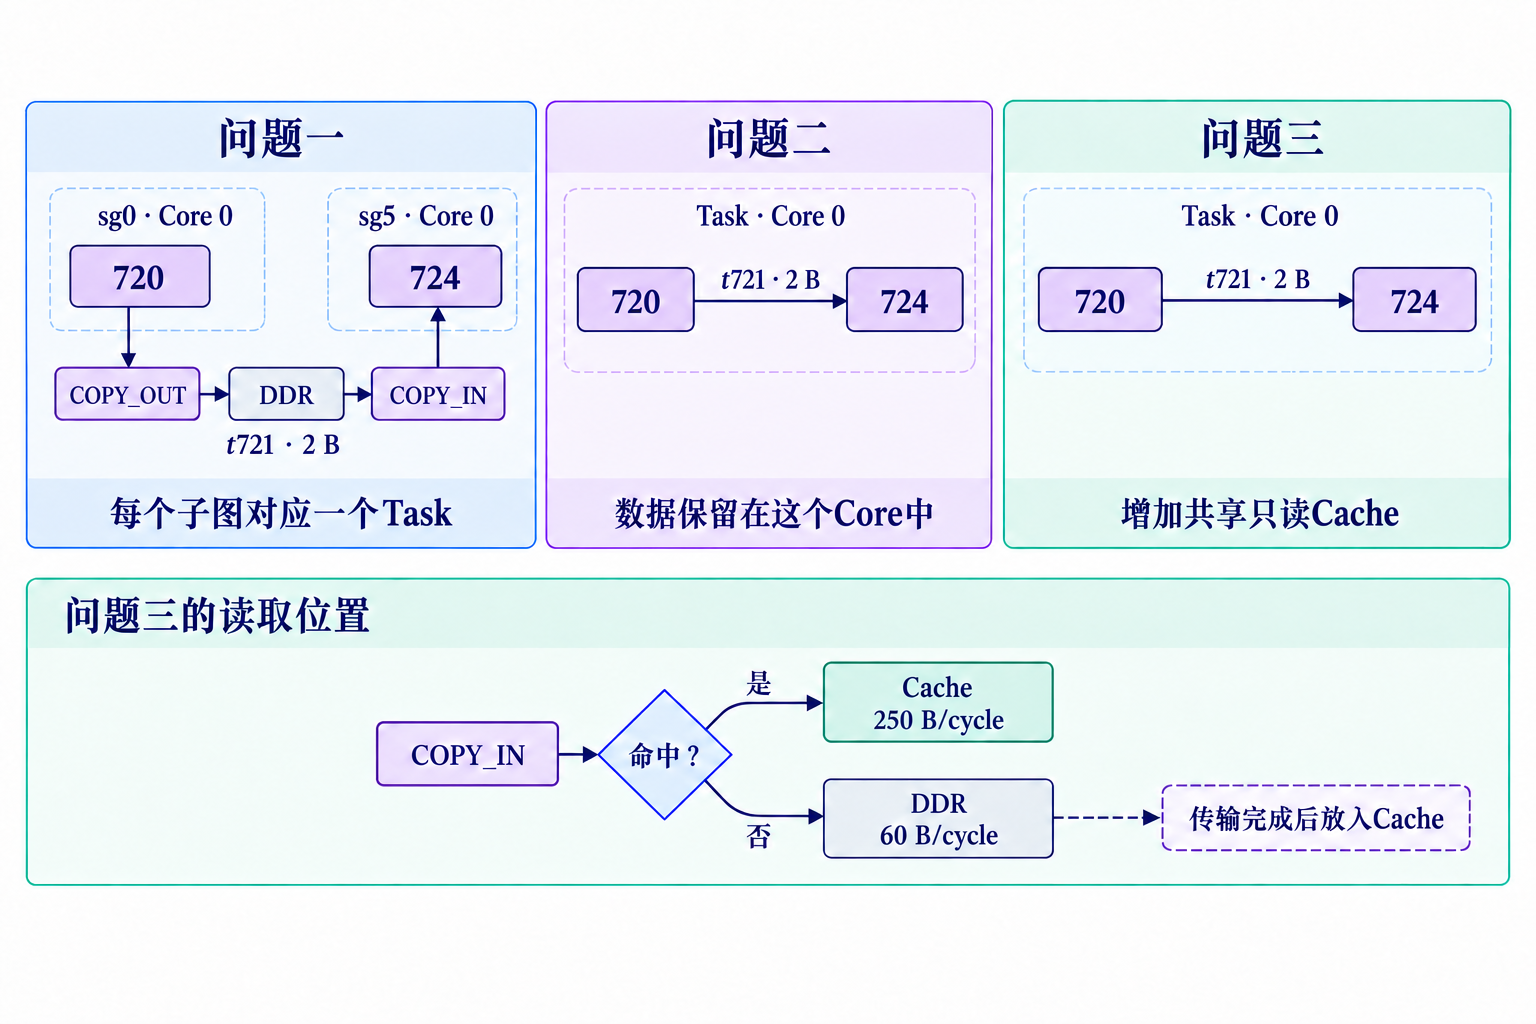
\includegraphics[width=\linewidth,height=.84\textheight,keepaspectratio]{figures/fig-progression-v3.png}
\caption{三问条件的差别。问题一为图中不同子图所对应的操作分别建立Task，数据经DDR中转；问题二允许同一个核心保留数据；问题三另为符合条件的COPY\_IN提供共享只读Cache。下部示意数据能够装入Cache时的读取过程；所有请求仍须满足原依赖及规定等待。}
\label{fig:progression}
\end{figure}

\subsection{多核调度中的核心挑战与求解思路}

综合题意与硬件执行特征，在通用神经网络处理器上实现高效的多核调度存在以下三项核心难点：

第一，\textbf{并行计算收益与跨核通信开销之间的非线性权衡}。将计算图拆解为更多子图并分散至更多核心，理论上能够提升计算单元的宏观并发度；然而，跨核心的数据交换必须插入额外的 \texttt{COPY\_OUT} 与 \texttt{COPY\_IN} 搬运操作。所有核心的 DDR 搬运操作均受制于总带宽仅为 60 字节/周期的共享内存通道，密集的跨核通信极易引发严重的内存带宽争用与同步停顿。如果因通信导致的额外 DDR 搬运与等待所增加的执行周期，超过了并行分配所节省的计算周期，多核方案的总完成时间反而会恶化。

第二，\textbf{片上私有缓存容量限制与数据驻留的动态约束}。在问题二和问题三中，将具有数据依赖的操作集中至同一核心能够避免外部内存搬运；然而，核心内部 L1 和 UB 的私有存储容量是严格受限的。核内调度在编译阶段若检测到局部缓存容量不足，会预先插入将数据换出至核外 DDR、后续再换入的溢出搬运操作（spill）。这不仅会增加额外的 DDR 搬运开销，若调度依赖安排不当还会导致方案无法推进。

第三，\textbf{局部核心排序与全局数据依赖交织下的死锁风险}。通过反例，我们可以说明为什么仅仅保证原始计算图无环并不能确保多核调度方案合法：假设核心 0 上的子图任务 \(S_1\) 需等待核心 1 上的子图任务 \(S_2\) 提供数据，而核心 1 内部指定的调度次序又要求先执行任务 \(S_3\) 再执行任务 \(S_2\)；若任务 \(S_3\) 恰好又间接依赖于任务 \(S_1\) 的运算结果，两个核心便会陷入``\(S_1\) 等待 \(S_2\)、\(S_2\) 等待 \(S_3\)、\(S_3\) 等待 \(S_1\)''的循环依赖状态，导致评测系统发生死锁。

针对上述挑战，本文遵循题面关于避免暴力迭代搜索、单用例高效求解的指导原则，设计了结构化的求解流程：

\begin{enumerate}
\def\labelenumi{\arabic{enumi}.}
\tightlist
\item
  \textbf{基于图结构的特征分析与候选构造}：分析计算图的连通分支、关键路径与张量复用关系，针对独立并行分支与数据密集型计算链，直接构造少量具有结构特征的完整候选方案；
\item
  \textbf{调度顺序的无环性判定}：将核心内子图执行次序作为时序边显式引入子图依赖图中，证明所给次序不产生有向环，确保方案满足依赖先后关系（需要说明的是，顺序无环是合法执行的必要条件，但仍需结合存储容量与完整评测进一步检验）；
\item
  \textbf{结合通信代价模型的理论下界快速剪枝}：基于题面给定的硬件流水线资源与通信带宽约束，计算理想并发条件下的时间下界与跨核通信开销，辅助快速筛除劣质候选；
\item
  \textbf{离散事件模拟选优}：在受限的评估预算内，调用评测程序对生成的完整候选方案进行离散事件模拟，从中选取 Makespan 最小的方案作为输出。
\end{enumerate}


\section{模型假设与符号说明}

\subsection{硬件参数与执行约束}

本文的建模与算法设计严格建立在题面给定的体系结构参数与官方离散事件评测程序的基础上。计算图中各算子的计算语义、操作类型及原始数据依赖保持不变，算法不得通过删减计算或修改运算结果来缩短完成时间。全部存储容量、总线带宽及同步等待常数均采用官方固定配置\cite{ref1}。

根据硬件配置参数，系统的主要物理约束如下：

\begin{enumerate}
\def\labelenumi{\arabic{enumi}.}
\tightlist
\item
  \textbf{核心数量}：可用核心数 \(K \in \{1, 2, 3, 4, 5\}\)，系统为各核心编号为 \(0, 1, \dots, K-1\)；
\item
  \textbf{片上私有缓存}：每个核心配备独立的局部存储器 L1 与统一缓冲区 UB，其存储容量分别为 \(524{,}288\text{ B}\)（\(512\text{ KiB}\)）与 \(131{,}072\text{ B}\)（\(128\text{ KiB}\)）。两级缓存各自独立管理，未分配的 L1 容量无法与 UB 共享；
\item
  \textbf{共享主存与缓存带宽}：所有核心访问核外主存（DDR）的读写操作共享统一的全局带宽池，总带宽固定为 \(60\text{ B/cycle}\)。在问题三中，引入容量为 \(1{,}048{,}576\text{ B}\)（\(1\text{ MiB}\)）的共享只读二级缓存（Level-2 Cache，简称 L2），命中 Cache 的读取操作使用专用的共享 Cache 读取带宽通道，总带宽为 \(250\text{ B/cycle}\)，该带宽与 DDR 带宽相互独立，不占用 DDR 带宽池；
\item
  \textbf{同步与切换延迟}：在问题一中，同一核心连续执行的相邻 Task 之间须等待 \(100\text{ cycles}\) 的切换时间；若一个 Task 依赖位于其他核心的前驱 Task，其启动时刻还须满足晚于前驱 Task 完成时刻至少 \(1000\text{ cycles}\) 的跨核同步延迟。在问题二和问题三中，由于同核子图合并为单一 Task，核心内部不存在 Task 切换延迟；跨核心依赖仅作用于具体数据搬运操作，目标核心的 \texttt{COPY\_IN} 需在源核心对应的 \texttt{COPY\_OUT} 完成后等待 \(500\text{ cycles}\) 方可参与就绪判断。这些常数由评测程序在对应的事件发生时检查，不直接等同于图上的固定边权重。
\end{enumerate}

评测程序采用离散事件模拟推进执行。对于流水线操作队列，算子严格按核内静态调度生成的偏序队列以先进先出（first in, first out，FIFO）方式推进就绪与发射。对于问题三中的只读 Cache，其缓存行维护独立的 FIFO 淘汰队列：当 Cache 剩余容量不足以容纳新载入的张量时，系统依次淘汰最早写入 Cache 的条目；后续核心读取 Cache 发生命中时，只读访问不会更新该条目在 FIFO 队列中的淘汰顺序。单张量物理大小超过 Cache 总容量（\(1\text{ MiB}\)）的数据不进入 Cache。

若核内调度算法在静态编译时评估到私有片上缓存（L1 或 UB）容量不足以容纳计算过程中的所有活跃张量，评测程序会在该核心的指令流中预先插入溢出搬运操作（spill），即通过 \texttt{PIPE\_MTE3} 将暂不使用的中间数据经由 DDR 写出，后续需要时再通过 \texttt{PIPE\_MTE2} 重新从 DDR 读入。溢出搬运会产生额外的 DDR 访问流量并占用共享带宽，调度方案应尽量平抑片上张量驻留峰值以减少溢出开销。

\subsection{原始张量、数据副本与逻辑标识}

在计算图的生命周期中，同一份数学数据在不同调度阶段可能对应不同的图节点与存储实体，我们明确区分以下三类对象：

\begin{enumerate}
\def\labelenumi{\arabic{enumi}.}
\tightlist
\item
  \textbf{原图张量节点}：指原始输入计算图 JSON 文件中给定的张量实体，具有唯一的整型 \texttt{id} 和固定的数据大小 \texttt{size}；
\item
  \textbf{调度生成的数据副本}：在多核心切分与核内调度阶段，当数据发生跨核心传输或因容量受限触发溢出时，评测程序会为该数据在不同存储介质（如源核心私有缓存、核外 DDR、目标核心私有缓存）中派生出新的物理数据实例。这些副本虽然承载相同的内容，但在物理上分别占用各自存储介质的独立空间；
\item
  \textbf{逻辑数据标识（\texttt{\seqsplit{logical\_tid}}）}：评测系统在处理问题三的只读 Cache 查询时，为所有源于同一张量派生出的物理副本赋予统一的逻辑标识 \texttt{\seqsplit{logical\_tid}}。当核心发起 \texttt{COPY\_IN} 搬运时，评测程序依据请求数据的 \texttt{\seqsplit{logical\_tid}} 查询 Cache 队列。若命中则直接从 Cache 读取，若未命中则在 DDR 读取完成后以该 \texttt{\seqsplit{logical\_tid}} 登记至 Cache 中。
\end{enumerate}

此外，方案合法性必须满足三重判定条件：

\begin{itemize}
\tightlist
\item
  \textbf{操作覆盖合法}：输入图中除 \texttt{COPY\_IN} 与 \texttt{COPY\_OUT} 之外的全部算子，均被无重复、无遗漏地指派至唯一的子图，且每个子图在 \texttt{\seqsplit{core\_schedules}} 中恰好出现一次；
\item
  \textbf{依赖拓扑无环}：子图间的数据依赖与各核心指定的子图执行顺序合并构成的扩展依赖图不存在有向环；
\item
  \textbf{存储与执行可行}：评测程序对方案能够成功完成核内调度并推进离散事件模拟，不因容量冲突或死锁导致模拟异常终止。
\end{itemize}

只有评测程序完整运行成功并输出日志的方案，其导出的 Makespan 才是有效指标。若方案因违反依赖或容量超限被评测程序拒绝，或者执行发生超时，均视为无效解，不将其填为零参与均值统计。

\subsection{主要符号}

本文使用的主要数学符号定义如下表所示。

{\def\LTcaptype{table} % do not increment counter
\begin{longtable}[]{@{}
  >{\raggedright\arraybackslash}p{(\linewidth - 4\tabcolsep) * \real{0.3333}}
  >{\raggedright\arraybackslash}p{(\linewidth - 4\tabcolsep) * \real{0.3333}}
  >{\raggedright\arraybackslash}p{(\linewidth - 4\tabcolsep) * \real{0.3333}}@{}}
\toprule\noalign{}
\begin{minipage}[b]{\linewidth}\raggedright
符号
\end{minipage} & \begin{minipage}[b]{\linewidth}\raggedright
定义说明
\end{minipage} & \begin{minipage}[b]{\linewidth}\raggedright
取值范围或量纲
\end{minipage} \\
\midrule\noalign{}
\endhead
\bottomrule\noalign{}
\endlastfoot
\(G=(O\cup T, E)\) & 原始计算图，其中 \(O\) 为操作节点集合，\(T\) 为张量节点集合，\(E\) 为有向依赖边集合 & 题面输入给定 \\
\(V\) & 待调度的计算算子集合（即 \(O\) 中操作类型不为 \texttt{COPY\_IN} 和 \texttt{COPY\_OUT} 的算子） & \(V \subset O\) \\
\(b_t, \ell_t\) & 数据张量 \(t\) 的物理大小（字节）及其预设存储位置（DDR、L1 或 UB） & \(b_t \in \mathbb{N}^+ \text{ (B)},\ \ell_t \in \{\text{DDR}, \text{L1}, \text{UB}\}\) \\
\(d_v, p_v\) & 算子 \(v\) 的硬件执行周期数及其所绑定的硬件执行管道 Pipe & \(d_v \ge 1 \text{ (cycle)},\ p_v \in \{\text{PIPE\_M}, \text{PIPE\_V}, \dots\}\) \\
\(K\) & 系统可用的计算核心总数 & \(K \in \{1, 2, 3, 4, 5\}\) \\
\(\pi(v)\) & 算子划分映射，表示算子 \(v\) 所归属的子图编号 & \(\pi: V \to \mathbb{N}\) \\
\(a(s)\) & 子图分配映射，表示子图 \(s\) 所指派执行的核心编号 & \(a: \mathcal{S} \to \{0, 1, \dots, K-1\}\) \\
\(\sigma_k\) & 核心 \(k\) 所承担的子图编号的有序调度列表 & 子图编号的全排列序列 \\
\(P=(\pi, a, \sigma)\) & 完整的多核切分与调度方案（对应提交 JSON 文件的两个字段） & 参赛提交规范 \\
\(q\) & 赛题问题编号 & \(q \in \{1, 2, 3\}\) \\
\(M_q(P)\) & 方案 \(P\) 在问题 \(q\) 的评测环境下运行所得的总体任务执行时间（Makespan） & cycle \\
\(D_q(P)\) & 方案 \(P\) 在评测程序下产生的总额外 DDR 数据搬运量 & B（字节） \\
\(B_i\) & 第 \(i\) 张计算图在官方基准单核心调度算法下的基线 Makespan & cycle \\
\(H_{i,K}\) & 第 \(i\) 张计算图在 \(K\) 个核心下运行问题三方案所得的 Cache 字节命中率 & \([0, 1]\) \\
\(L, U\) & 在相同图输入、核心数与硬件配置下，对所有合法方案均成立的理论下界与已有合法方案的时间上界 & cycle \\
\(L(P)\) & 仅在指定候选方案 \(P\) 的特定结构约束下成立的时间下界（不作为全局下界） & cycle \\
\(U/L\) & 当前最佳方案的 Makespan 与理论下界之比，用于评估当前方案逼近理论极限的程度 & 无量纲比值 \\
\(T_{\text{solve}}\) & 求解算法从读取输入到输出合法方案文件的端到端墙钟运行时间 & s（秒） \\
\end{longtable}
}

在官方输入文件中，非核外搬运计算算子 \(v \in V\) 的 \texttt{cycles} 字段可能为 0。根据官方评测程序逻辑，计算单元在单核心执行推进时确保每个计算算子至少占用 1 个执行时钟周期，因此在建立数学分析模型与计算计算负载下界时，算子执行周期定义为 \(d_v = \max(1, \text{cycles}_v)\)（单位为 cycle）。需要特别说明的是，\(d_v\) 仅适用于具备固定计算时长的算子集合 \(V\)；对于核外数据搬运操作（\texttt{COPY\_IN} 与 \texttt{COPY\_OUT}），其执行耗时由张量大小 \(b_t\) 与实时动态共享带宽池决定，不适用该静态公式。

\subsection{评价指标及统计方法}

\subsubsection{1. 方案质量指标与平均加速比}

多核心调度方案的质量首要由 Makespan \(M_q(P)\) 衡量。为了评估多核并行化相对于单核执行的性能提升程度，根据题面第 5 页脚注 2 的明确规定，多核心调度方案的平均加速比（Speedup）采用逐用例比值的算术平均方法进行计算：

\begin{equation}
\bar{S}_{q,K} = \frac{1}{100} \sum_{i=1}^{100} \frac{B_i}{M_q(P_{i,K})},
\end{equation}

其中 \(B_i\) 为官方评测系统针对第 \(i\) 张图在单核心条件下的基线 Makespan，\(P_{i,K}\) 为算法针对第 \(i\) 张图在 \(K\) 个核心下生成的调度方案。必须说明的是，平均加速比是逐图加速比值的算术平均值，而非全部用例单核时间总和除以多核时间总和。题面官方基线 \(B_i\) 由通用的单核启发式调度算法给出，并不保证是单核条件下的数学全局最优解，因此在部分用例中可能出现加速比略大于核心数 \(K\) 的情况。

对于问题三，题面要求评估引入只读 Cache 带来的相对性能增益。评测时保持问题三所生成的调度方案 \(P\) 完全不变，分别在启用 Cache 和关闭 Cache（即回退至问题二纯 DDR 模式）两种配置下运行评测程序，分别记录其 Makespan 为 \(M_3(P)\) 和 \(M_2(P)\)。单用例的 Cache 加速比定义为 \(M_2(P) / M_3(P)\)，多用例汇总时同样报告这 100 对结果比值的算术平均值。

\subsubsection{2. 额外数据搬运量与缓存命中率}

次要方案质量指标包括数据搬运量与缓存命中率：

\begin{itemize}
\tightlist
\item
  \textbf{总额外 DDR 数据搬运量 \(D_q(P)\)}：官方评测程序统计调度后执行的所有 \texttt{COPY\_IN} 和 \texttt{COPY\_OUT} 搬运字节总数，减去原始计算图固有输入输出张量所需的基准搬运字节数。在问题三中，官方评测系统保持相同的统计口径，并不在 Cache 命中时将该统计字段直接扣减，因此该字段反映的是切分引入的总通信需求，而非物理 DDR 总线的实际净流量；
\item
  \textbf{Cache 字节命中率 \(H\)}：定义为命中 Cache 的数据总字节数占所有发起 Cache 查询的总数据字节数的比例，即 \begin{equation}
H = \frac{\text{hit\_bytes}}{\text{hit\_bytes} + \text{miss\_bytes}}.
\end{equation} 当用例中不存在任何可查询的 \texttt{COPY\_IN} 操作时，官方程序将分母为零的情形约定为 \(H = 0\)。该指标严格按字节量统计，而非按访问请求的发生次数统计。
\end{itemize}

\subsubsection{3. 求解效率与原题时限解读}

算法的求解效率通过端到端求解时间 \(T_{\text{solve}}\) 评估，度量从程序启动、解析输入图 JSON，到完成拓扑分析、方案构造、内部筛选及输出方案文件全过程的实际物理墙钟耗时（Wall-clock Time）。

原题第 5 页脚注 1 指出：``此处`高效地'代表着算法应该避免使用暴力迭代搜索机制，以单个用例能在 5～10 分钟内给出结果为佳。''我们对该项要求的理解为：

\begin{itemize}
\tightlist
\item
  该项表述属于针对求解算法工程效率与设计理念的指导性建议，强调算法应当利用计算图的固有结构与硬件特性进行针对性构造，避免盲目的大规模蒙特卡洛枚举或无剪枝的暴力迭代；
\item
  5～10 分钟是算法在常规计算硬件上的用例级运行耗时建议，并非超过 600 秒即被判定无效的硬性淘汰线，亦非要求算法必须耗满 5 分钟方可输出。本队算法在保证方案高质量的前提下，追求极高的求解速度，单用例求解耗时通常控制在数秒至数十秒之间。
\end{itemize}

\subsubsection{4. 评测程序的角色与调用账目}

在算法求解与评测交付中，明确区分在线候选评分（作为求解算法的一部分用于分支决策，计入求解墙钟时间）与外部官方复评（求解完成后独立运行以验证方案合法性并输出最终官方主成绩）：

\begin{itemize}
\tightlist
\item
  \textbf{E0（官方离散事件评测程序）}：官方提供的未修改基准评测脚本（\texttt{\seqsplit{code/multicore\_cut\_evaluate\_problem\_*.py}}）。在问题三求解过程中，算法基于归约树排序理论生成有限个候选方案后，直接调用 E0 进行在线完整打分验证（单用例调用预算上限为 3 次）；而在外部复评阶段，本文汇报的所有主实验成绩、最终 Makespan 以及附录逐用例结果，均以 E0 的独立运行输出为最终确认标准；
\item
  \textbf{E1（批量精确评估工具）}：队内依据官方规则实现的轻量级独立评估实现。在问题一求解器中，用于对有限个候选方案（包括基础划分、局部调整及分支重分配方案）进行在线模拟打分与选优，单用例在线调用次数严格限制在至多 10 次以内；
\item
  \textbf{E2（场景二轻量精确评估工具）}：队内针对问题二场景（同核子图合并为单一 Task、跨核以 COPY 依赖推进）实现的快速评估工具（在固定源码 \texttt{\seqsplit{src/q2\_nikolastarx/}} 中由 \texttt{\seqsplit{SceneBEvaluator}} 提供支持）。在问题二求解器（\texttt{\seqsplit{adaptive\_hypergap\_guarded.py}}）中，算法基于超图多阶段划分与空隙插入构造出 baseline、gap 与 hypergap 等有限候选后，调用在线评分适配器进行打分（单用例在线调用上限为 3 次），并根据所返回的 Makespan 与额外数据搬运量自适应选取最佳方案；若 E2 接口调用异常则自动回退至 E0。
\end{itemize}

所有求解器内部的在线打分调用及其等待时间均严格计入算法的端到端求解时间 \(T_{\text{solve}}\) 中，未在求解阶段隐瞒在线评价开销。


\section{计算图切分与调度模型}

\subsection{多核切分与调度决策的形式化表示}

多核心调度算法的核心任务是在满足数据流依赖与硬件物理约束的前提下，共同确定算子到子图的分组、子图到计算核心的指派以及各核心内部子图任务的执行先后时序。

设 \(V \subset O\) 为原始计算图中除跨边界核外搬运操作 \texttt{COPY\_IN} 与 \texttt{COPY\_OUT} 之外的待调度操作集合（此集合包含全部计算算子以及子图内部的数据搬运操作）。方案的三个决策维度形式化定义如下：

\begin{enumerate}
\def\labelenumi{\arabic{enumi}.}
\tightlist
\item
  \textbf{算子划分映射 \(\pi\)}：\(\pi: V \to \mathcal{S}\) 为每个算子 \(v \in V\) 分配一个子图编号，所有非空子图组成的集合记为 \(\mathcal{S}\)；
\item
  \textbf{核心分配映射 \(a\)}：\(a: \mathcal{S} \to \{0, 1, \dots, K-1\}\) 为每个子图 \(s \in \mathcal{S}\) 指定负责处理该子图计算任务的核心编号；
\item
  \textbf{核心内调度序列 \(\sigma_k\)}：对于每个核心 \(k \in \{0, 1, \dots, K-1\}\)，\(\sigma_k\) 为指派给该核心的子图子集 \(\{s \in \mathcal{S} \mid a(s) = k\}\) 给出一个严格的全序执行排列。
\end{enumerate}

三项决策共同构成了完整的多核心切分与调度方案，记为三元组 \(P = (\pi, a, \sigma)\)。该数学表示与官方提交契约（\texttt{\seqsplit{contest\_io.py}}）中的持久化结构完全对应：\texttt{\seqsplit{node\_to\_subgraph}} 字段直接对应映射 \(\pi\)，\texttt{\seqsplit{core\_schedules}} 字段直接对应核心执行序列集合 \(\{\sigma_k\}_{k=0}^{K-1}\)。单有算子分组而不指定执行核心，或者指定了分配而不确定同一核心上的执行次序，均无法在底层评测系统中推进离散事件时钟。

为了严谨刻画多核心场景下由数据依赖与核心内排队顺序交织构成的时序先后关系，我们建立子图层级的扩展有向拓扑：

\begin{itemize}
\tightlist
\item
  \textbf{子图间数据依赖边集 \(E_{\mathcal{S}}\)}：若子图 \(s\) 内算子与子图 \(t\) 内算子之间存在直接操作依赖（op-to-op）、跨子图张量生产---消费关系，或经由官方派生逻辑生成的完整跨边界数据搬运路径（\(s \ne t\)），则在子图之间引入一条有向依赖边 \((s, t) \in E_{\mathcal{S}}\)；
\item
  \textbf{核心内执行次序边集 \(E_\sigma\)}：若在某个核心的执行序列 \(\sigma_k\) 中，子图 \(s\) 紧邻排定在子图 \(t\) 之前执行，则引入一条有向调度时序边 \((s, t) \in E_\sigma\)。
\end{itemize}

将两类有向边与子图顶点集 \(\mathcal{S}\) 合并，构成\textbf{加入同一核心顺序后的子图依赖图}：

\begin{equation}
D^+(P) = (\mathcal{S}, E_{\mathcal{S}} \cup E_\sigma).
\end{equation}

若该有向图中存在有向环，则说明子图之间的数据流动与核心内的排队规则发生了冲突，方案在官方前置派生与校验阶段（如 \texttt{\seqsplit{stub\_multicore\_cut\_and\_schedule.py}} 第 220 行对商图环路的检查）将因违反子图无环或执行顺序约束而被直接拒绝；在问题一的独立任务硬件语义下，此类冲突将直接表现为不同核心任务之间的循环等待。在图划分与多处理器调度领域，将具有先后依赖的计算划分并保持商图（quotient graph）无环以及核心间负载平衡，是受到广泛关注的课题\cite{ref6}；然而，通用无环图划分工具通常针对静态割权或通信量建模，不能直接推导本题包含复杂硬件延迟与动态访存仲裁下的 Makespan 保证。

在方案满足拓扑无环性及格式规范的前提下，官方评测程序针对具体问题场景 \(q \in \{1, 2, 3\}\) 执行离散事件模拟推进 \(\mathcal{E}_q(P)\)，生成方案在规定硬件环境下的性能评估向量 \((M_q(P), D_q(P), H_q(P))\)，其中 \(M_q(P)\) 为总体任务执行时间（Makespan，单位为 cycle），\(D_q(P)\) 为额外 DDR 数据搬运量（单位为 Byte），\(H_q(P)\) 为问题三特有的 Cache 字节命中率。

设 \(\mathcal{F}_q(G, K)\) 为评测程序能够顺利推进并正常完成的所有合法方案集合，多核心调度问题的数学优化模型表述为：

\begin{equation}
\min_{P \in \mathcal{F}_q(G, K)} M_q(P).
\end{equation}

多核心调度方案的官方评价目标（题面 §1.3--1.4）是以最小化任务总体执行时间（Makespan）\(M_q(P)\) 为首要优化目标，同时考察额外 DDR 数据搬运量（官方以相对单核基线的额外数据搬运量 \(\text{extra\_ddr\_bytes}\) 统计）；对于问题三，官方评测程序同时报告基于字节统计的 Cache 命中率 \(H_3(P)\)。字典序比较并非官方评价指标的法定公式，而是本队求解器在面临多个候选方案时采用的内部择优与回退保护规则：在问题一与问题二中，算法在候选方案之间按主次目标进行比较（其中问题一在候选调度器内部按 \((M_1(P), \text{scheduled\_copy\_bytes})\) 排序择优，最终在官方口径下折算为相对单核基线的 \(\text{extra\_ddr\_bytes}\)；问题二在离散模拟评估后按 \((M_2(P), D_2(P))\) 字典序改善择优）；在问题三中，算法则严格以缩短 Makespan（\(M_3(P) < U\)）作为是否采纳 Cache 专用重排方案的门槛准则。

\subsection{三个问题的通用求解策略与递进关系}

求解该多核调度问题的根本难点在于：图论意义上的局部启发式指标（如划分割边权重、计算量均匀度）无法准确反映带有动态带宽争用与复杂同步等待的微架构执行过程；然而，若对搜索空间中的海量可能切分逐一运行完整的离散事件模拟评测，其时间开销在工程上又是不可接受的。

为了在合理的时间内产出高质量方案，本文设计了一套通用的结构化求解流程：

\begin{enumerate}
\def\labelenumi{\arabic{enumi}.}
\tightlist
\item
  \textbf{图拓扑特征分析}：分析原始计算图的连通分支、长程关键路径以及张量复用聚集度，提取适合多核心展开的天然结构单元；
\item
  \textbf{结构化候选方案构造}：针对提取出的拓扑特征，直接生成少量包含切分、核心分配与执行顺序的完整候选方案 \(P = (\pi, a, \sigma)\)；
\item
  \textbf{拓扑合法性与无环性校验}：构建扩展依赖图 \(D^+(P)\)，校验所有待调度算子的无遗漏覆盖以及子图任务执行时序的无环性；
\item
  \textbf{条件支持的下界评估与剪枝}：在支持下界计算的特定算法分支中（如问题三中使用基于流水线计算工作量的下界估计），结合算子异构计算量与依赖拓扑评估候选方案潜力，提前过滤劣质构造；
\item
  \textbf{受限预算下的离散事件模拟选优}：对通过筛选的少量优质候选方案，调用离散事件评测程序获取模拟性能指标，自适应输出 Makespan 最小的方案。
\end{enumerate}

图 \ref{fig:framework} 展示了该通用求解流程，三类问题的算法分支共享统一的输入解析、拓扑校验与闭环选优机制。

\begin{figure}[!htbp]
\centering
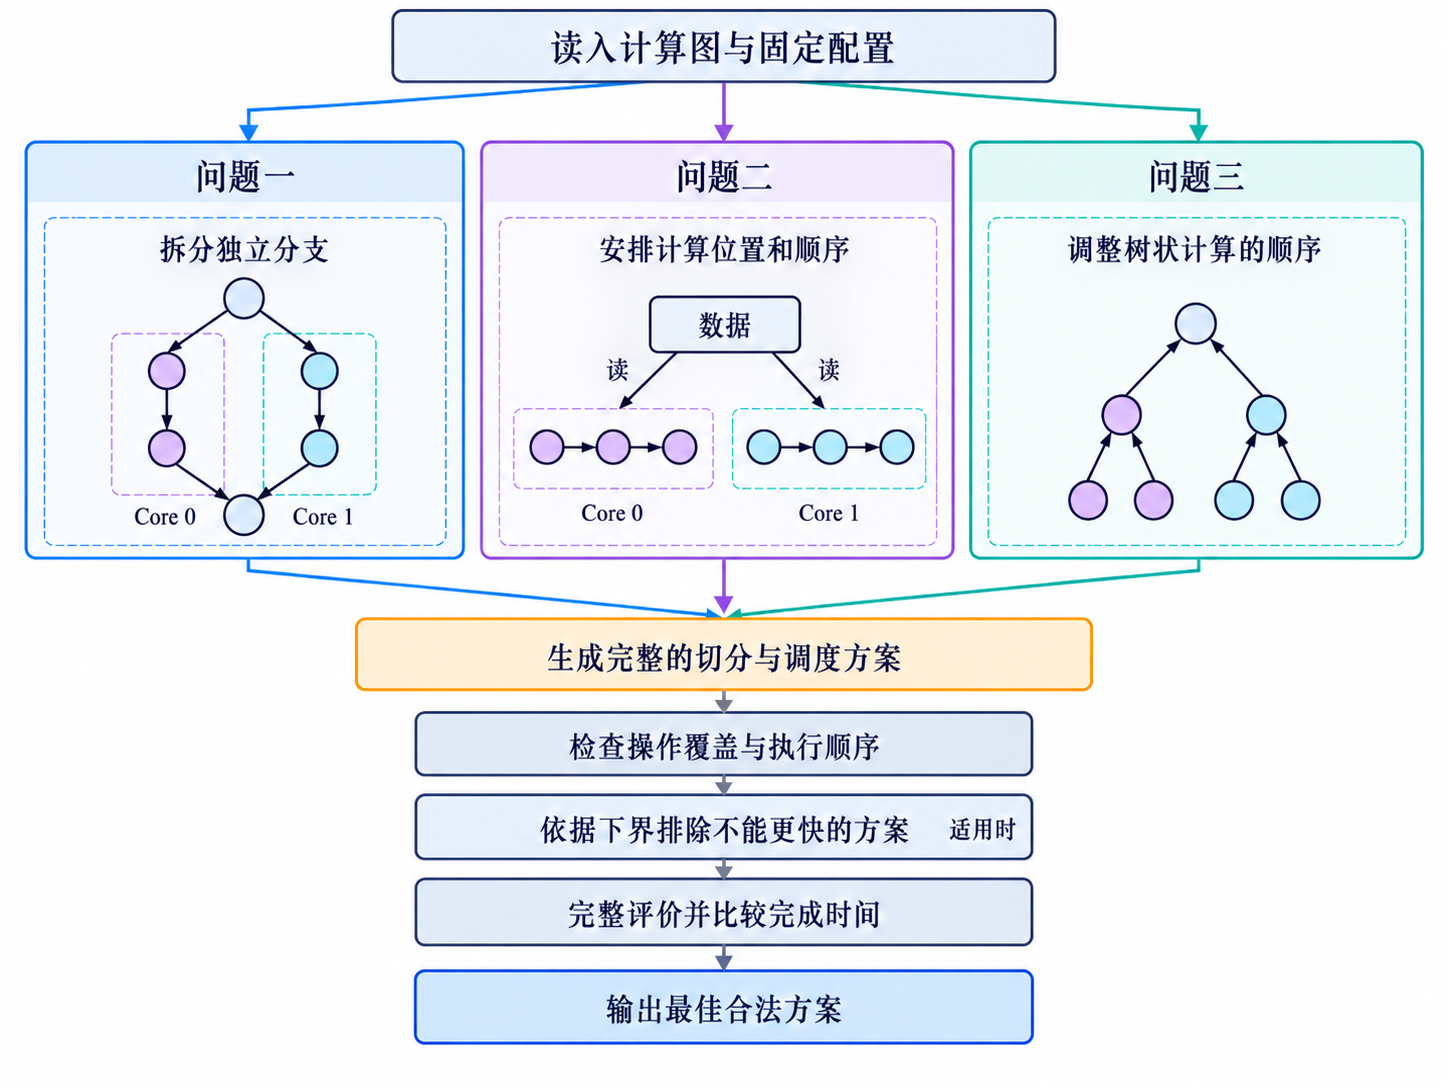
\includegraphics[width=\linewidth,height=.84\textheight,keepaspectratio]{figures/fig-framework-v2.png}
\caption{三问共用的方案构造与比较步骤。各分支只在结构条件满足时采用，所形成的完整方案需检查依赖与容量，并通过执行评价比较完成时间。下界只在其证明条件成立时用于提前排除候选。}
\label{fig:framework}
\end{figure}

根据题面硬件执行语义的演变，三类问题的具体构造策略呈现清晰的递进逻辑：

\begin{itemize}
\tightlist
\item
  \textbf{问题一（子图隔离执行）}：每个子图独立封装为一个硬件 Task，子图间数据无法片上保留，通信代价高昂。算法侧重于识别无数据依赖的并行支路，通过分支重新分配均衡各核心的计算负载，平衡并行度与 DDR 通信开销；
\item
  \textbf{问题二（同核子图合并）}：同一核心上的全部子图合并为单一 Task，允许片上私有缓存直接跨子图复用数据。算法基于超图划分理论，将具有密集张量复用的算子归并至同一核心，以减少跨核心边界的数据通信，并在局部最小割过程中通过按流水线的工作量上限保护机制防止计算向单核过度倾斜；该工作量保护并不构成消除 Step 2 缓存换入换出（spill）的容量证明，方案的物理表现由后续评测综合决定；
\item
  \textbf{问题三（引入共享只读 Cache）}：在问题二合并执行的基础上增加核外只读 L2 Cache。针对多核心读取共享数据的树状归约结构，算法基于深度优先排序理论排定子树计算次序，在非交错执行模型下降低限定模型内部峰值；最终的 Cache 字节命中率与整图 Makespan 仍由官方离散事件模拟评测器综合评定。
\end{itemize}

\subsection{子图划分与执行顺序的无环性判定}

通过以下反例，我们可以说明为什么仅仅保证原始计算图无环以及每个子图内部无环，并不能确保多核心调度方案可安全执行。

假设原始计算图包含四个计算算子 \(a_1, a_2, b_1, b_2\)，它们之间仅存在两条数据依赖边 \(a_1 \to b_1\) 与 \(b_2 \to a_2\)。显然，原始计算图是一个严格的有向无环图。若算法将算子划分为两个子图 \(S_A = \{a_1, a_2\}\) 与 \(S_B = \{b_1, b_2\}\)，并分别分配至核心 0 与核心 1 执行。此时，子图依赖商图同时存在由 \(S_A\) 到 \(S_B\) 的依赖（\(a_1 \to b_1\)）以及由 \(S_B\) 到 \(S_A\) 的依赖（\(b_2 \to a_2\)）。无论两个核心内部如何排定子图的执行次序，该方案都会因违反官方子图无环与执行顺序约束而在前置派生阶段被直接拒绝；在问题一的独立硬件任务执行语义下，核心 0 上的任务与核心 1 上的任务更将陷入相互等待对方完成的循环等待。不仅如此，即便子图间仅存在单向数据流动，若核心内部指定的调度序列引入了反向时序边，两类边叠加后同样会使扩展依赖图成环并被系统拦截。

因此，在对候选方案进行深入评价之前，必须形式化判定其扩展依赖图 \(D^+(P)\) 的无环性。

\textbf{命题3.1（无环性充分条件）。} 设 \(P = (\pi, a, \sigma)\) 为一份多核心切分与调度方案，其对应的扩展依赖图为 \(D^+(P) = (\mathcal{S}, E_{\mathcal{S}} \cup E_\sigma)\)。若存在一个标号函数 \(r: \mathcal{S} \to \mathbb{Z}\)，使得对于图中任意有向边 \((s, t) \in E_{\mathcal{S}} \cup E_\sigma\)，均满足 \begin{equation}
r(s) < r(t),
\end{equation} 则该扩展依赖图 \(D^+(P)\) 必然不存在有向环，方案中的子图任务能够排定出合法的拓扑执行序列。

\begin{proof} 采用反证法。假设 \(D^+(P)\) 中存在一个由 \(m\) 个子图构成的有向环 \(s_1 \to s_2 \to \cdots \to s_m \to s_1\)（其中 \(m \ge 2\)）。根据命题假设，环上的每一条有向边 \((s_i, s_{i+1})\) 均满足严格的大小偏序关系： \begin{equation}
r(s_1) < r(s_2) < \cdots < r(s_m) < r(s_1).
\end{equation} 由此直接导出 \(r(s_1) < r(s_1)\)，出现数学逻辑矛盾。因此，假设不成立，\(D^+(P)\) 中必然不存在有向环。 \end{proof}

需要明确的是，标号函数 \(r\) 是用于证明执行顺序不存在循环互锁的拓扑排序判据，而非用于衡量调度性能的评分函数。通过有序块号与标号偏序证明商图无环性在无环 DAG 划分数学建模中有着经典应用\cite{ref7}。通过该判定仅证明了调度时序在依赖关系上的无环可行性；方案在实际推进中是否会出现片上缓存超限或评测异常，仍须通过后续的离散事件模拟进行完整验证。

\subsection{总体任务执行时间下界与候选剪枝准则}

为了在受限时间内高效筛选候选解，我们需要建立问题固有的理论时间下界。在异构流水线与多核心调度中，简单的贪心启发式排程容易引发多处理器调度异例（例如增加资源或减少局部耗时反而增大全局完成时间）\cite{ref2}；因此需要结合物理必要不等式推导严格的完成时间下界。

固定输入图 \(G\)、核心总数 \(K\) 以及问题编号 \(q\)。若对于集合 \(\mathcal{F}_q(G, K)\) 中的任意合法方案 \(P\)，其 Makespan 均满足 \(M_q(P) \ge L\)，则称 \(L\) 为该问题的\textbf{完成时间下界（lower bound on makespan）}，其单位为时钟周期（cycle）。

我们通过考察所有合法方案都必须完成的固有计算工作量与依赖链长，推导一个全局基础下界：

\begin{enumerate}
\def\labelenumi{\arabic{enumi}.}
\tightlist
\item
  \textbf{计算算子子集与周期定义}：设 \(V_{\mathrm{comp}} \subseteq V\) 为具有确定执行时长的计算算子集合，它由绑定在矩阵流水线 \texttt{PIPE\_M}（Cube 单元）与向量流水线 \texttt{PIPE\_V}（Vector 单元）上的计算操作构成，其算子固有计算耗时严格定义为 \(d_v = \max(1, \text{cycles}_v)\)（单位为 cycle）。集合 \(V \setminus V_{\mathrm{comp}}\) 中的数据搬运与内存访问操作耗时取决于底层总线仲裁、动态带宽争用与缓存状态，不具有静态固定常数周期；若输入图中缺乏某一特定流水线操作（例如 \(V_M = \emptyset\) 或 \(V_V = \emptyset\)），则对应阶段的总工作量取为边界值 0（即 \(W_M = 0\) 或 \(W_V = 0\)）；
\item
  \textbf{异构计算负载下界}：Cube 密集型计算算子集合记为 \(V_M \subseteq V_{\mathrm{comp}}\)，Vector 密集型计算算子集合记为 \(V_V \subseteq V_{\mathrm{comp}}\)。其总计算量分别为 \(W_M = \sum_{v \in V_M} d_v\) 与 \(W_V = \sum_{v \in V_V} d_v\)（cycle）。由于全系统包含 \(K\) 个计算核心，且每个核心均配备物理独立的 \texttt{PIPE\_M} 与 \texttt{PIPE\_V} 硬件执行流水线，受算子不可切分及局部依赖约束，零通信理想调度的最优执行时长并不必然等于工作量除以核心数；但任何合法方案完成各流水线计算所需的时间绝不可能低于工作量均分下界，即 \(\lceil W_M / K \rceil\) 与 \(\lceil W_V / K \rceil\) 构成了矩阵与向量计算的必要下界。由于两类计算流水线采用物理分离的执行单元，其计算负载不能简单相加除以 \(K\)；
\item
  \textbf{关键路径依赖下界}：在由全体计算算子 \(V_{\mathrm{comp}}\) 构成的依赖关系中，若算子 \(u\) 的输出张量直接或通过中间数据搬运操作传递给算子 \(v\) 读取，则存在从 \(u\) 到 \(v\) 的计算依赖路径。需要说明的是，将原始图中跨核心数据搬运链（COPY 路径）投影或折叠为计算算子间的依赖弧，仅在满足附录 B.1 经官方评测代码验证的硬件同步与依赖推导语义下成立，不能无条件断言任意复杂搬运链均可简单等价缩点；定义从源点算子到汇点算子沿任意经核验的计算依赖路径累加各算子计算时长 \(d_v\) 的最大值为\textbf{关键路径长度} \(L_{\mathrm{cp}}\)（cycle），该累加严格计入路径终点算子的计算时长 \(d_v\)。由于同一依赖链上的算子在逻辑上必须依次串行执行，任何合法方案的全局执行时间必然不低于 \(L_{\mathrm{cp}}\)。
\end{enumerate}

综合上述约束，针对全局所有合法方案成立的理论基础下界为：

\begin{equation}
L_{\mathrm{basic}} = \max\left\{L_{\mathrm{cp}},\ \left\lceil\frac{W_M}{K}\right\rceil,\ \left\lceil\frac{W_V}{K}\right\rceil,\ \max_{v\in V_{\mathrm{comp}}}d_v\right\} \le M_q(P).
\end{equation}

当特定流水线操作集合为空时，其对应分量取为 0。

除了适用于全部方案的全局下界外，针对某一具体候选方案 \(P = (\pi, a, \sigma)\)，若考虑其特定的子图分配、各核心实际承担的算子工作量峰值以及跨核心传输所必需的最低延迟，可以推导出针对该方案的特定下界 \(L(P) \le M_q(P)\)。

基于特定下界 \(L(P)\)，可建立针对主目标的\textbf{理论剪枝判据}：假设在求解过程中算法已获得一份经过模拟评测确认的合法方案 \(P_0\)，其 Makespan 记为当前性能上界 \(U = M_q(P_0)\)。若后续搜索旨在寻找 Makespan 严格更短的解（即满足 \(M_q(P) < U\)），由于 \(M_q(P) \ge L(P)\)，一旦新候选方案 \(P\) 的特定下界满足 \begin{equation}
L(P) \ge U,
\end{equation} 则必然有 \(M_q(P) \ge U\)，该候选在完成时间维度绝无可能严格超越 \(P_0\)。需要指出的是，若在相同周期时允许通过次要目标（减少额外搬运量 \(D_q(P)\)）选优，则在 \(L(P) = U\) 的边界情形下，下界无法直接排除该候选产生更小搬运量的可能性；因此该理论剪枝严格针对于单一 Makespan 维度的快速淘汰。在实际算法实现中，由于离散事件评测本身具有较大开销，全局理论下界并未作为三个问题统一执行的硬性搜索剪枝器，而是在具备确定下界推导的特定算法分支（如问题三中的流水线计算下界）中作为辅助判据；各题主要通过轻量级结构校验与有限高质量候选策略来规避无效搜索。

若 \(L\) 为全局下界，\(\mathrm{OPT}\) 为当前用例在给定核心数下的未知数学最优值，而 \(U\) 为算法所得最佳方案的实际 Makespan，三者在量纲上均为 cycle 且满足 \(L \le \mathrm{OPT} \le U\)。当 \(L > 0\) 时，同量纲相除得到无量纲的最优性相对间隙上界：

\begin{equation}
\frac{U - \mathrm{OPT}}{\mathrm{OPT}} \le \frac{U - L}{L} = \frac{U}{L} - 1.
\end{equation}

比值 \(U/L\) 直观量化了当前方案距离理论极限的逼近程度。比值越接近 1，表明所得调度方案越充分地挖掘了硬件算力潜能。

\subsection{求解时间的组成与计算复杂度}

求解程序的运行效率通过物理墙钟时间进行度量，它与底层离散事件模拟时钟周期（Makespan）具有本质不同的物理内涵。

求解程序的端到端运行时间 \(T_{\mathrm{solve}}\)（以秒为单位）由以下五个执行阶段构成：

\begin{equation}
T_{\mathrm{solve}} = T_{\mathrm{parse}} + T_{\mathrm{construct}} + T_{\mathrm{check}} + \sum_{j=1}^{b} T_j + T_{\mathrm{IO}},
\end{equation}

其中：

\begin{itemize}
\tightlist
\item
  \(T_{\mathrm{parse}}\) 为输入计算图 JSON 文件的解析与数据结构初始化时间；
\item
  \(T_{\mathrm{construct}}\) 为针对特定问题场景生成有限候选方案的算法构造时间；
\item
  \(T_{\mathrm{check}}\) 为算子覆盖合法性与扩展依赖图 \(D^+(P)\) 无环性判定时间；
\item
  \(b\) 为算法在求解当前用例期间实际调用的在线离散事件评测次数，\(T_j\) 为第 \(j\) 次在线评测的运行耗时；
\item
  \(T_{\mathrm{IO}}\) 为将最终优选方案持久化写入标准输出 JSON 文件的磁盘交互时间。
\end{itemize}

在计算复杂度层面：

\begin{enumerate}
\def\labelenumi{\arabic{enumi}.}
\tightlist
\item
  \textbf{拓扑解析与无环校验}：设待调度算子数为 \(|V|\)，直接与间接数据依赖边数为 \(|E_V|\)，生成的子图数量为 \(|\mathcal{S}|\)。扩展依赖图 \(D^+(P)\) 的构建与基于 Kahn 算法的有向无环性判定均可在 \(O(|V| + |E_V| + |\mathcal{S}|)\) 的线性时间内高效完成；
\item
  \textbf{结构候选构造与软预算约束}：结构化构造主要包含连通分量遍历、前沿划分与支路重分配检查。各算法针对深层结构分析设定了显式计算上限（例如问题一中支路重分配限制任务数不超过 320，并引入 2.0 秒的结构分析软预算退出检查，避免在极端复杂图上耗费过多时间）；
\item
  \textbf{离散事件模拟评测开销}：单次离散事件评测耗时 \(T_j\) 取决于评测内核在推进离散事件时的队列操作与硬件模拟规模。在实际求解测试中，若采取盲目迭代搜索，随着评估次数累加，总时间将迅速失控。本文各求解器将单用例的在线评测调用次数 \(b\) 严格冻结在固定调用上限内（问题一至多 10 次，问题二与问题三至多 3 次），大幅削减了在线评测的时间占比；结合轻量级结构校验，实测端到端运行时间整体落在题面所建议的高效区间内。
\end{enumerate}


\section{问题一：子图独立执行场景下的多核切分与调度}

\subsection{硬件执行语义与多核调度的权衡机制}

在问题一的系统设定中，每个非空子图 \(s \in \mathcal{S}\) 均被底层编译系统独立封装为一个物理硬件任务（Task）。由于子图之间在硬件执行层面上严格隔离，芯片私有缓存无法实现跨 Task 的数据保留。无论两个具有数据依赖关系的 Task 最终被指派至同一个计算核心还是不同的计算核心，它们之间传递的中间数据张量均必须通过外部主存（DDR）进行持久化中转，即由前驱 Task 将生成张量执行 \texttt{COPY\_OUT} 写出至 DDR，再由后继 Task 执行 \texttt{COPY\_IN} 从 DDR 读回片上缓存。

设 Task \(s\) 在指派核心 \(a(s)\) 上的开始执行时刻与完成时刻分别为 \(A_s\) 和 \(F_s\)（单位为 cycle）。记 \(\mathrm{prev}(s)\) 为排定在同一核心上紧邻 \(s\) 之前执行的 Task，\(\operatorname{pred}(s)\) 为在数据依赖关系上先于 \(s\) 执行的全部前驱 Task 集合。底层离散事件评测系统对硬件调度时序施加了如下物理约束：

\begin{equation}
A_s \ge F_{\mathrm{prev}(s)} + \Delta_{\mathrm{local}}, \quad \Delta_{\mathrm{local}} = 100 \text{ cycles},
\end{equation}

\begin{equation}
A_s \ge F_t + \Delta_{\mathrm{sync}}, \quad \forall t \in \operatorname{pred}(s) \text{ 且 } a(t) \ne a(s), \quad \Delta_{\mathrm{sync}} = 1000 \text{ cycles}.
\end{equation}

其中，\(\Delta_{\mathrm{local}} = 100\) cycles 为同一核心上相邻任务间的上下文切换开销；\(\Delta_{\mathrm{sync}} = 1000\) cycles 为跨核心依赖同步屏障引入的硬件等待时延。若某项约束中的前驱对象不存在，则对应不等式不生效。

上述时序约束揭示了多核心切分与调度决策中的基本权衡关系（trade-off）：

\begin{enumerate}
\def\labelenumi{\arabic{enumi}.}
\tightlist
\item
  \textbf{并行收益与排队削减}：将互无计算依赖的算子划分至不同的子图并分配给多个计算核心，能够让无依赖的算子在物理分离的流水线（\texttt{PIPE\_M} 与 \texttt{PIPE\_V}）上并发推进。虽然这并不改变由原始数据依赖所决定的固有关键路径长度，但能够显著缩短由于单核执行资源有限而被强制串行化的排队等待时间；
\item
  \textbf{通信开销与同步代价}：若子图切分引入了跨子图的数据流动边界，中间数据张量必须通过 DDR 进行读写传递，从而产生额外的数据搬运开销与总线争用；当数据依赖跨越不同核心时，更会触发长达 1000 cycles 的跨核同步屏障等待。此外，若多个核心并发访问 DDR，还可能引发内存总线带宽争用，增加各 Task 的实际等待时间。
\end{enumerate}

因此，多核心切分并非越细越好。只有当并发执行所节省的排队等待周期足以弥补切分所引入的 DDR 搬运与跨核同步开销时，切分方案才能实现全局执行时间的净收益。

\subsection{结构化候选方案生成与多级细化策略}

基于上述物理权衡，算法首先分析输入计算图的数据流动特征。若仅考虑算子之间的直接与间接计算依赖，能够沿无向连通边相互到达的算子子集构成了一个弱连通分量（weakly connected component）。不同连通分量之间天然不存在计算依赖，但在读取共享外部输入时仍可能产生总线访问争用。

针对该计算图结构，算法参考前序研发建立的分叉阶段与前沿子树划分策略，在统一求解入口（\texttt{unified.py}）中设计了六类互补的基础结构候选生成器。针对给定用例与核心数 \(K\)，求解器至多构造六种不同侧重点的基础方案：

\begin{enumerate}
\def\labelenumi{\arabic{enumi}.}
\tightlist
\item
  \textbf{连通分量前沿划分与大任务重组（\texttt{bounded}）}：首先调用树状前沿划分模块（\texttt{\seqsplit{tree\_frontier.py}}，参数 \texttt{\seqsplit{packet\_factor=4}}）生成初始划分；随后对操作数超过 4096 的巨型任务进行内部扫描，在不切断任何依赖链的前提下识别其内部独立的计算连通分量，按目标约 1024 个算子的粒度安全重组为独立子图，作为基础参考方案；
\item
  \textbf{大工作量后缀波次剥离（\texttt{\seqsplit{heavy-or-sink}}）}：当单个主要分量在主导流水线上的计算量占比达到或超过 80\% 且分量数充足时，将该瓶颈分量的末端汇点算子剥离为粗粒度后缀波次（若不满足触发条件则回退至分层剥离汇点算子的 \texttt{sink\_peel} 候选）；
\item
  \textbf{过载连通分量切分（\texttt{overload}）}：针对单个连通分量在任一流水线上的计算工作量超过全系统平均核心公摊配额的情形，将其剥离出的独立算子包按负载均衡启发式分配至轻载核心，摊薄瓶颈核心的计算压力；
\item
  \textbf{共享输入开销感知划分（\texttt{\seqsplit{shared-input}}）}：当连通分量数不小于核心数且外部输入张量总大小超过 \(524{,}288 \text{ B} = 512 \text{ KiB}\) 时，统计各分量对外部输入数据的共享重叠度，将重度共享同一张量的分量优先归并至同一核心，以抑制重复 DDR 搬运总量；
\item
  \textbf{前沿子树划分与并行展开（\texttt{\seqsplit{fork-frontier}}）}：采用前序研发建立的分叉阶段与前沿子树划分策略，并推广至无分叉链及内向树（in-trees）结构，沿拓扑阶段以前沿粒度（\texttt{grain=4}）将不相交的子树打包分配至各核心，挖掘拓扑天然存在的横向并行性；
\item
  \textbf{受限链状结构私有化（\texttt{\seqsplit{capacity-return}}）}：严格识别私有的矩阵-向量链-矩阵模式（\(M \to V^+ \to M\) 且矩阵算子数恰为分量数 2 倍），在片上缓存容量满足保守估算的前提下进行局部紧凑分组，规避中间向量张量的外存溢出。
\end{enumerate}

图 \ref{fig:fang-fork} 给出了一个三核心（\(K=3\)）场景下的典型分叉汇聚（fork-join）计算图的任务切分与分配构型示意。该图仅用于阐释多核心任务切分、核心分配以及执行次序的形式化拓扑关系，并非底层的真实执行时间轴，亦不代表特定用例的独立支路迁移候选。计算图由源头计算 \(s \to a\) 出发，分叉为三条互无计算依赖的并行支路：支路一（\(b_1 \to c_1 \to d_1\)）、支路二（\(b_2 \to d_2\)）与支路三（\(b_3 \to c_3 \to d_3\)），最终汇总至汇聚计算 \(r \to t\)。系统将其划分为 5 个任务并分配给 3 个计算核心：

\begin{itemize}
\tightlist
\item
  核心 0 负责 Task 0（包含 \(s, a\)）与 Task 1（包含 \(b_1, c_1, d_1\)）；
\item
  核心 1 负责 Task 2（包含 \(b_2, d_2\)）与 Task 4（包含 \(r, t\)）；
\item
  核心 2 负责 Task 3（包含 \(b_3, c_3, d_3\)）。 图中实线有向边表示指派在同一核心内部的任务执行先后次序，虚线有向边表示跨越不同核心的任务间数据依赖。在问题一的系统规则下，所有任务边界之间的数据流转均须通过外部主存（DDR）中转，跨核心依赖还会引入跨核硬件同步时延。
\end{itemize}

\begin{figure}[!htbp]
\centering
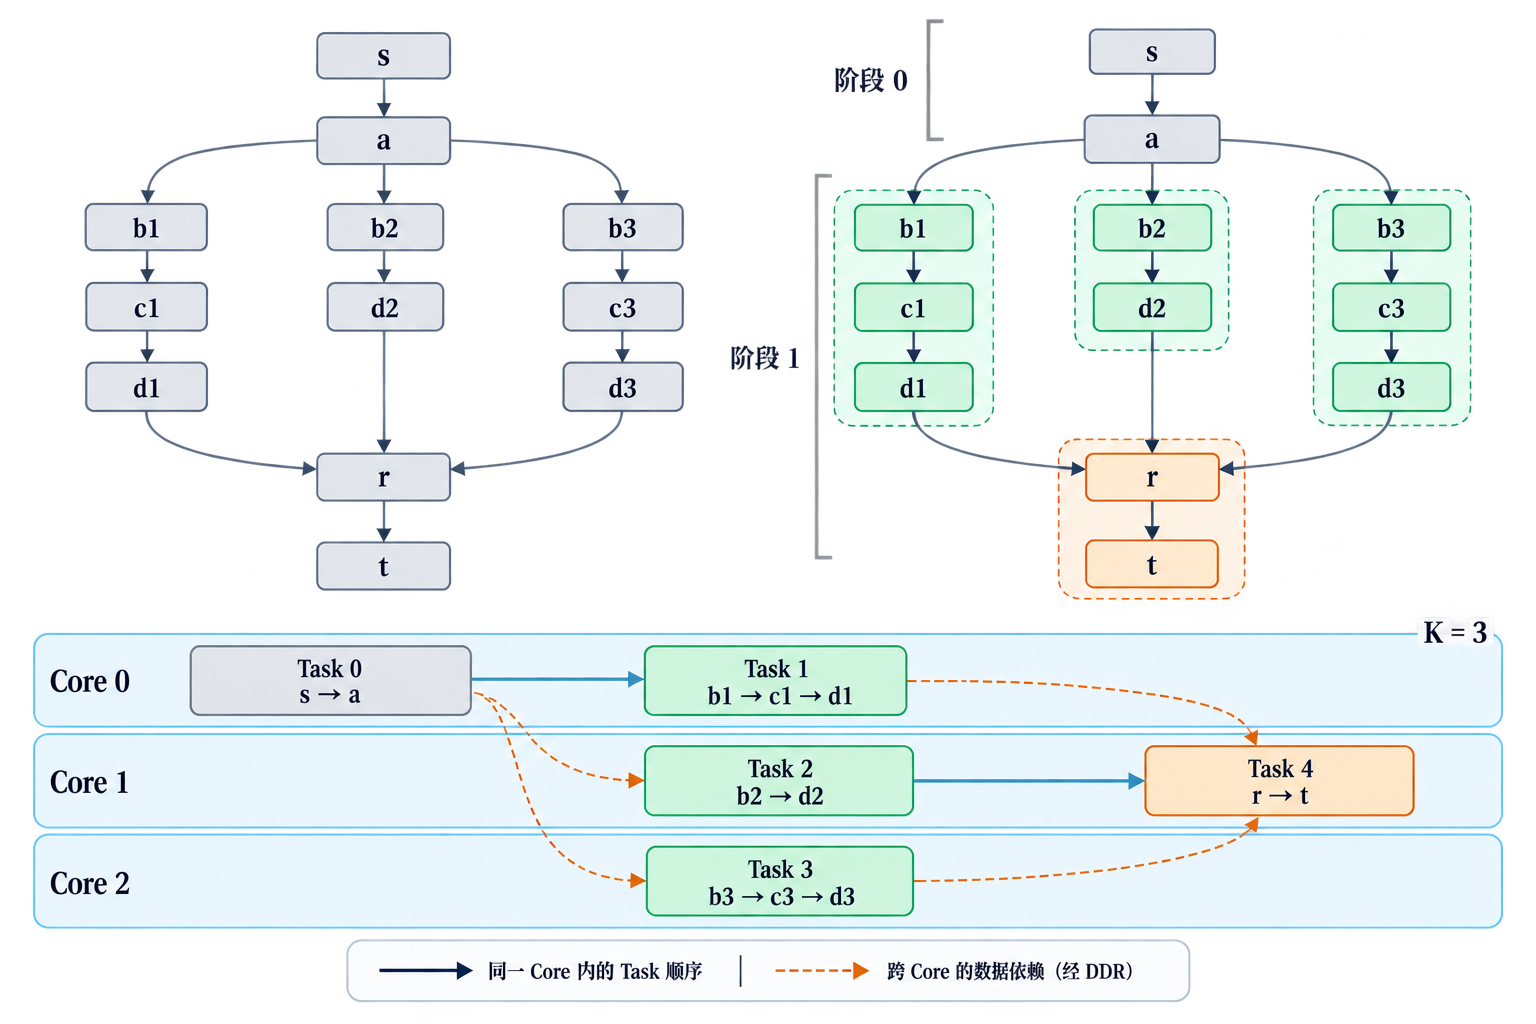
\includegraphics[width=\linewidth,height=.84\textheight,keepaspectratio]{figures/fig4-2-fang-A.png}
\caption{三核心场景下的分叉汇聚结构任务划分与多核分配示意。包含 5 个 Task 与 3 个计算核心（核心 0 处理 Task 0 与 Task 1，核心 1 处理 Task 2 与 Task 4，核心 2 处理 Task 3）。实线有向边表示同一核心内部的执行全序，虚线有向边表示跨核心的任务数据依赖，所有 Task 边界的数据流动均通过外部主存（DDR）中转。}
\label{fig:fang-fork}
\end{figure}

在上述基础方案的基础上，求解器通过两级进阶细化模块展开多级候选探索：

\begin{itemize}
\tightlist
\item
  \textbf{动态分组长度细化与拓扑保形顺序（\texttt{\seqsplit{structural\_refine.py}}）}：在基础候选选优结果的基础上，一方面对链状流水结构进行分组长度调整（至多产生 1 次在线评测）；另一方面尝试 \texttt{paced} 与 \texttt{\seqsplit{root-heavy-fused}} 两种拓扑保形执行次序（至多产生 2 次在线评测），从中优选出性能最佳的父级方案 \(P_{\mathrm{parent}}\)；
\item
  \textbf{分支援助重分配（\texttt{\seqsplit{branch\_aid.py}} \& \texttt{\seqsplit{branch\_refine.py}}）}：针对父级方案中各核心在同一拓扑阶段负载失衡的情形，通过桥树分析识别可转移的独立计算分支，将其重分配至空闲核心（至多产生 1 次在线评测）。
\end{itemize}

全流程严格采用精确模拟器 E1 进行在线评分与方案筛选，且每一阶段均执行完整的字节级哈希去重与格式合法性校验。未产生新结构或与已有方案完全重复的候选不参与评测，全流程在线 E1 评测调用次数严格限制在 10 次以内。

\begin{figure}[!htbp]
\centering
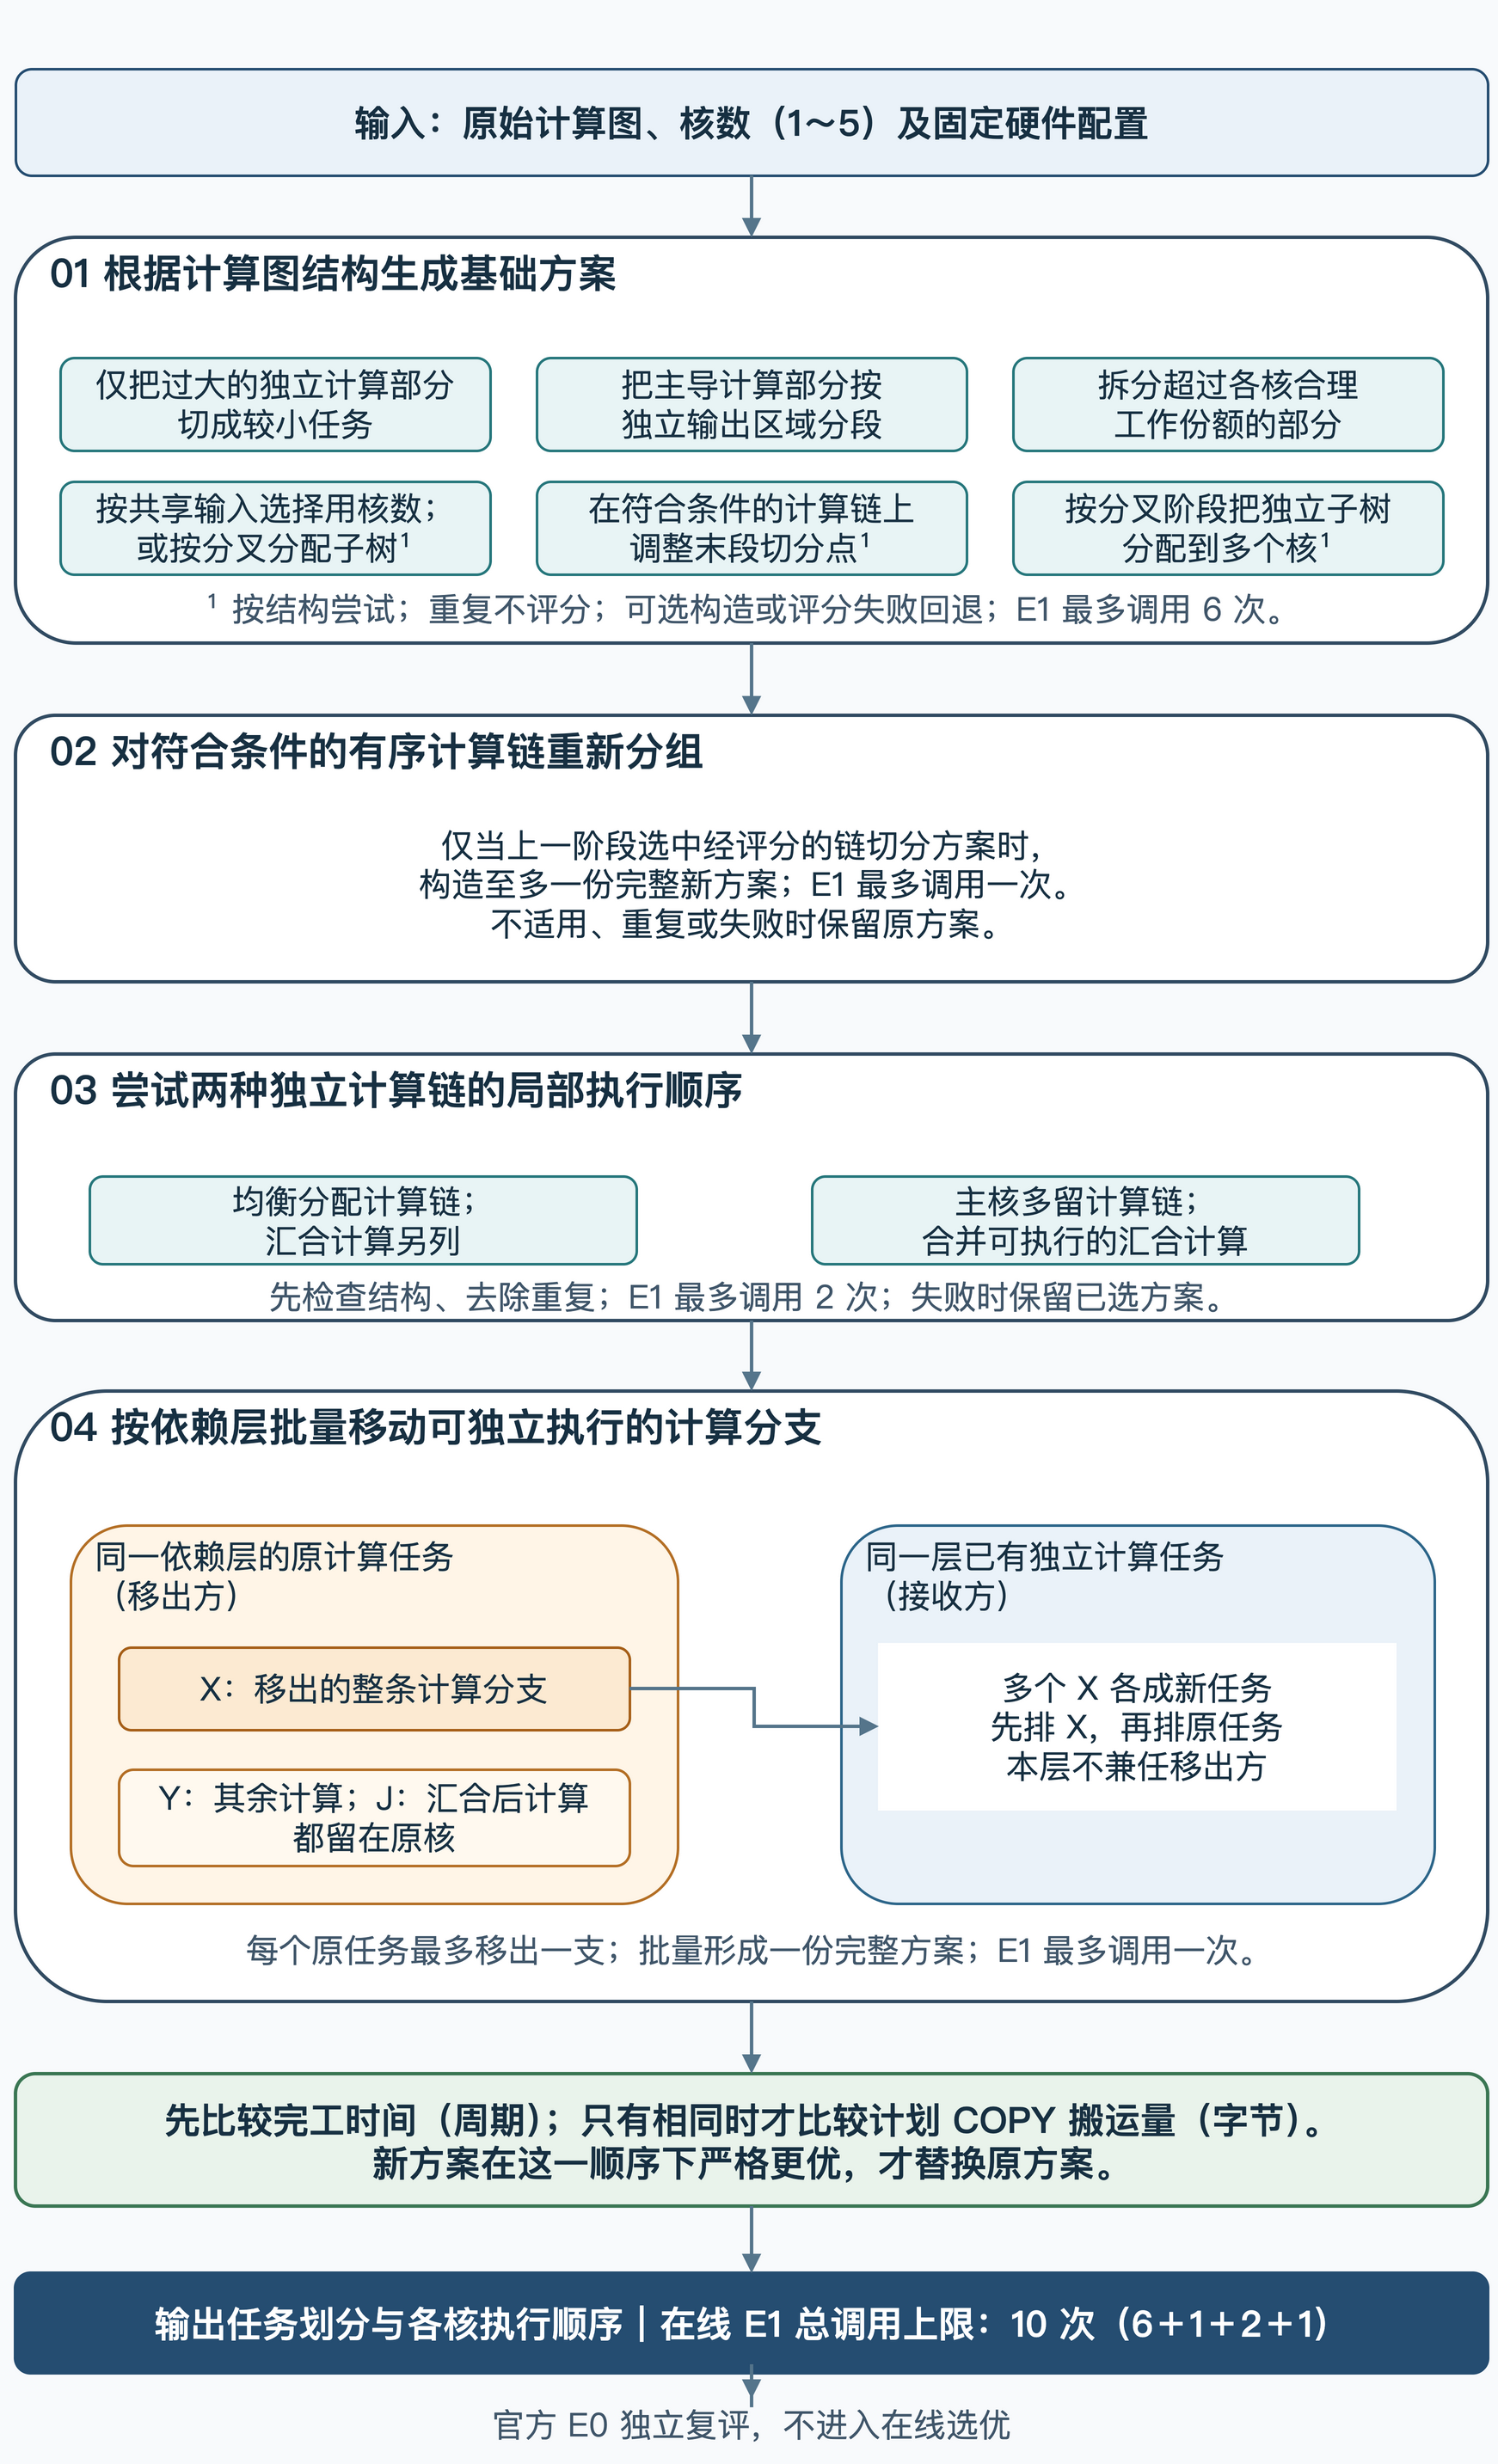
\includegraphics[width=\linewidth,height=.84\textheight,keepaspectratio]{figures/p1-834-flow-clean.png}
\caption{问题一固定算法的全流程构造与评测选优逻辑。展示六类基础候选生成、两级细化阶段的在线 E1 评测守卫与逐阶段择优规则，全流程评测调用上限为 10 次，最终方案由 E0 独立复评验证。}
\label{fig:p1-complete-flow}
\end{figure}

\begin{figure}[!htbp]
\centering
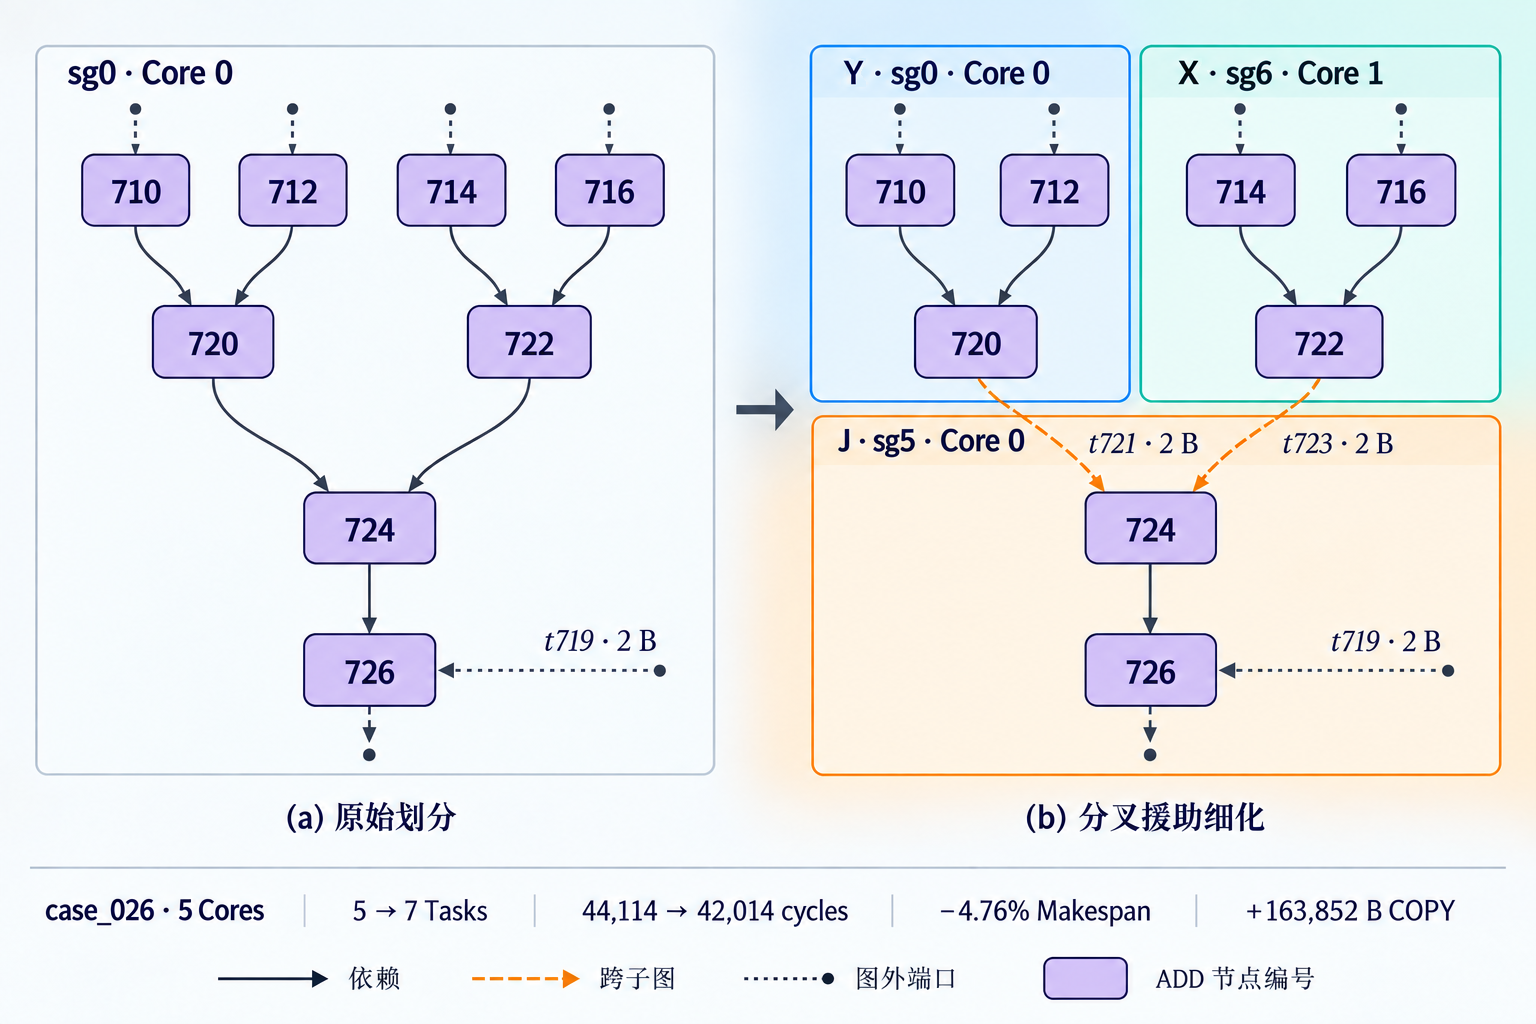
\includegraphics[width=\linewidth,height=.84\textheight,keepaspectratio,trim=0 235 0 0,clip]{figures/fig-p1-cuts-xy-corrected.png}
\caption{case\_026、5个核心的真实归约片段。左为原始划分，右为将独立支路改分到另一个核心；八个 ADD 节点的编号和依赖不变。点线端口连接裁剪范围外的输入或后继，橙色虚线为位于不同子图中的操作之间的依赖。}
\label{fig:p1-cuts}
\end{figure}

\subsection{分支援助重分配机制与无环性形式化证明}

为了在不打破原有稳定调度结构的前提下进一步压低瓶颈核心的执行延迟，本文设计了分支援助重分配机制（Branch-Aid）。该机制以 \texttt{\seqsplit{structural\_refine}} 输出的优秀方案作为父级解 \(P_{\mathrm{parent}} = (\pi_0, a_0, \sigma_0)\)，仅在多核心场景（\(2 \le K \le 5\)）下尝试对同阶段核心负载进行横向均衡。

\subsubsection{拓扑波次与援助角色判定}

算法将父方案中的全部 \texttt{COPY} 节点暂时收缩，构建关于 Task 顶点的有向依赖图 \(G_{\mathrm{task}} = (\mathcal{S}_0, E_{\mathcal{S}_0})\)。对于每个 Task \(s \in \mathcal{S}_0\)，定义其拓扑高度（height）为从任意源点 Task 出发到达 \(s\) 的最长依赖路径边数：

\begin{equation}
h(s) = \begin{cases} 0, & \text{若 } \operatorname{pred}(s) = \emptyset, \\ 1 + \max_{t \in \operatorname{pred}(s)} h(t), & \text{若 } \operatorname{pred}(s) \ne \emptyset. \end{cases}
\end{equation}

算法要求父方案必须严格满足\textbf{波次单调推进性质}：在每一个核心 \(k\) 的执行序列 \(\sigma_{0,k}\) 中，Task 的执行次序必须沿高度 \(h\) 严格单调递增，即若 Task \(s\) 排定在 Task \(t\) 之前，则必有 \(h(s) < h(t)\)。因此，在任意固定高度 \(h\) 处，每个核心至多分配有一个 Task。将高度为 \(h\) 的全部 Task 构成的集合记为波次 \(W_h\)。

算法遍历每个波次 \(W_h\)，并检查以下强约束条件：

\begin{enumerate}
\def\labelenumi{\arabic{enumi}.}
\tightlist
\item
  \textbf{同波次无依赖条件}：在波次 \(W_h\) 内部，来自不同核心的 Task 之间不得存在任何直接或间接的计算算子数据依赖，即不同核心在该阶段处理的计算任务在拓扑上完全独立；
\item
  \textbf{流水线负载统计与角色划分}：统计波次 \(W_h\) 内各核心在各个实际出现的执行流水线上的有效计算工作量 \(\operatorname{work}(c)[p] = \sum_{v \in T_{h, c}, \operatorname{pipe}(v) = p} \max(1, \operatorname{cycles}_v)\)，确定该波次全系统工作量最大的主导流水线 \(p^*\)。在流水线 \(p^*\) 上计算量显著超过核心平均工作量的核心被判定为\textbf{捐赠核心候选（donor candidates）}；计算量低于平均值且在波次 \(W_h\) 处分配有原有独立任务 \(T_{\mathrm{orig}}\) 的核心被判定为\textbf{援助核心候选（helper candidates）}。捐赠核心集与援助核心集严格互斥，且在该波次没有分配任务的核心不参与援助；
\item
  \textbf{桥树（Bridge-Tree）分解与算子三相划分}：在捐赠核心的原始任务 \(T_{\mathrm{donor}}\) 内部，通过 Tarjan 算法寻找无向图中的桥边，并将桥边割开后的各个双边连通块压缩为节点，构建\textbf{桥树（bridge tree）}（而非基于割点的块割树）。若存在唯一的内部汇点算子，且存在一个汇聚算子 \(j \in T_{\mathrm{donor}}\) 恰好接收两条来自独立前驱的桥边输入，则将 \(T_{\mathrm{donor}}\) 严格划分为三个互不相交的算子子集：

  \begin{itemize}
  \tightlist
  \item
    \textbf{导出独立支路 \(X\)}：由其中一条前驱支路及其全部上游算子构成的独立连通块，被选定为迁移至援助核心的子图；
  \item
    \textbf{保留独立支路 \(Y\)}：由另一条前驱支路、其余上游算子以及该 Task 内可能存在的其他独立连通分量构成，继续保留在原捐赠核心上执行；
  \item
    \textbf{汇合计算部分 \(J\)}：由汇聚算子 \(j\) 及其在 \(T_{\mathrm{donor}}\) 内部的全部后继后代算子构成，继续保留在原捐赠核心上执行。
  \end{itemize}
\end{enumerate}

\subsubsection{依赖关系与全序构建规则}

三相划分在算子依赖结构上严格满足：

\begin{itemize}
\tightlist
\item
  \(X \cap Y = \emptyset\)，\(X \cap J = \emptyset\)，\(Y \cap J = \emptyset\)，且 \(X \cup Y \cup J = T_{\mathrm{donor}}\)；
\item
  \(X\) 与 \(Y\) 之间不存在任何正向或反向的数据依赖边；
\item
  所有跨子集依赖边均由 \(X\) 指向 \(J\) 或由 \(Y\) 指向 \(J\)；\(J\) 绝不存在指向 \(X\) 或 \(Y\) 的反向反馈边；
\item
  \(X\) 与 \(Y\) 的所有外部前驱算子均来自高度严格小于 \(h\) 的前驱波次任务。
\end{itemize}

在调度序列重构中，算法支持一个援助核心在同一波次批量接收来自不同捐赠核心的多个独立导出支路 \(X_1, X_2, \dots, X_m\)：

\begin{itemize}
\tightlist
\item
  \textbf{捐赠核心的执行时序}：原 Task \(T_{\mathrm{donor}}\) 所在位置被替换为子图 \(Y\) 与子图 \(J\) 的顺次执行，即在捐赠核心上 \(Y\) 紧邻排定在 \(J\) 之前（\(Y \to J\)）；
\item
  \textbf{援助核心的执行时序}：援助核心在执行其原有波次任务 \(T_{\mathrm{orig}}\) 之前，优先顺次排定执行其接收到的全部导出支路 \(X_1, X_2, \dots, X_m\)，即援助核心上的执行序列构型为 \(X_1 \to X_2 \to \cdots \to X_m \to T_{\mathrm{orig}}\)；
\item
  \textbf{核心内波次推进时序}：在每个核心的本地调度序列中，任务严格按高度递增排列，不同高度的任务顺序受本地排队序列与跨核数据依赖约束，并非在全芯片施加全局物理同步屏障。
\end{itemize}

\subsubsection{扩展依赖图无环性证明}

\textbf{命题4.1（分支援助重分配的无环性）。} 在上述波次推进、同波次独立性、三相依赖分解以及调度构建规则下，重分配后的新方案 \(P_{\mathrm{new}}\) 所诱导的扩展依赖图 \(D^+(P_{\mathrm{new}}) = (\mathcal{S}, E_{\mathcal{S}} \cup E_\sigma)\) 必然不存在有向环。

\begin{proof} 根据命题 3.1，只需构造一个严格单调的整数标号函数 \(r: \mathcal{S} \to \mathbb{Z}\)，使得图中的每一条有向边 \((u, v) \in E_{\mathcal{S}} \cup E_\sigma\) 均满足 \(r(u) < r(v)\)。

对于任意子图 \(s \in \mathcal{S}\)，设其在原始依赖图中所归属的波次高度为 \(h(s)\)。为每个波次 \(h\) 分配基准标号区间 \([100h, 100h + 99]\)。在波次 \(h\) 内部，针对不同角色子图定义整数标号如下：

\begin{enumerate}
\def\labelenumi{\arabic{enumi}.}
\tightlist
\item
  对于任意援助核心 \(c \in H_h\)，设其接收到的导出支路序列为 \(X_1, X_2, \dots, X_m\)。由于每个捐赠核心至多导出一个分支 \(X\) 且捐赠核心与援助核心互斥，必有 \(m \le |D_h| \le K - 1 \le 4 < 10\)。其原有的波次任务记为 \(T_{\mathrm{orig}}\)。定义： \begin{equation}
r(X_i) = 100h + 10 + i, \quad \forall i \in \{1, 2, \dots, m\},
\end{equation} \begin{equation}
r(T_{\mathrm{orig}}) = 100h + 30;
\end{equation}
\item
  对于任意捐赠核心 \(c \in D_h\)，其分裂出的子图为 \(Y\) 与 \(J\)。定义： \begin{equation}
r(Y) = 100h + 10, \quad r(J) = 100h + 40;
\end{equation}
\item
  对于既非援助核心亦非捐赠核心的正常核心上的原有任务 \(T_{\mathrm{norm}}\)，定义： \begin{equation}
r(T_{\mathrm{norm}}) = 100h + 20.
\end{equation}
\end{enumerate}

现在逐一验证扩展依赖图 \(D^+(P_{\mathrm{new}})\) 中的所有可能边 \((u, v)\)：

\begin{itemize}
\tightlist
\item
  \textbf{情形一：跨波次边}。

  \begin{itemize}
  \tightlist
  \item
    对于数据依赖边 \((u, v) \in E_{\mathcal{S}}\)：若 \(u\) 与 \(v\) 属于不同波次，由于 Task 拓扑高度的定义，所有外部前驱的高度严格小于后继任务的高度，故必有 \(h(u) \le h(v) - 1\)。因此 \(r(u) \le 100h(u) + 50 \le 100(h(v) - 1) + 50 = 100h(v) - 50 < 100h(v) + 10 \le r(v)\)，整数标号严格递增；
  \item
    对于同一核心上的调度次序边 \((u, v) \in E_\sigma\)：由于新方案严格保持波次单调推进，不同波次间的调度边同样满足 \(h(u) < h(v)\)，故必然有 \(r(u) < r(v)\)。
  \end{itemize}
\item
  \textbf{情形二：同波次内的核心调度边 \((u, v) \in E_\sigma\)}。

  \begin{itemize}
  \tightlist
  \item
    在援助核心上，调度序列为 \(X_1 \to X_2 \to \cdots \to X_m \to T_{\mathrm{orig}}\)。根据标号赋值，显然有 \(r(X_1) < r(X_2) < \cdots < r(X_m) < r(T_{\mathrm{orig}}) = 100h + 30\)；
  \item
    在捐赠核心上，调度序列为 \(Y \to J\)。根据定义，\(r(Y) = 100h + 10 < r(J) = 100h + 40\)；
  \item
    其余核心在波次 \(h\) 内至多只有一个任务，不存在同波次调度边。
  \end{itemize}
\item
  \textbf{情形三：同波次内的数据依赖边 \((u, v) \in E_{\mathcal{S}}\)}。

  \begin{itemize}
  \tightlist
  \item
    根据同波次无依赖假设，波次 \(h\) 内不同原始任务之间不存在任何计算依赖边；
  \item
    唯一可能存在同波次数据依赖边的仅为由原任务分裂出的子图对。根据三相划分的依赖性质：

    \begin{itemize}
    \tightlist
    \item
      若边为 \(X_i \to J\)，则 \(r(X_i) \le 100h + 20 < 100h + 40 = r(J)\)；
    \item
      若边为 \(Y \to J\)，则 \(r(Y) = 100h + 10 < 100h + 40 = r(J)\)；
    \item
      \(X_i\) 与 \(Y\) 之间无依赖边；\(J\) 绝无指向 \(X_i\) 或 \(Y\) 的依赖边；
    \item
      导出支路 \(X_i\) 与援助核心原有任务 \(T_{\mathrm{orig}}\) 原本分属不同的独立任务，二者之间不存在任何数据依赖边。
    \end{itemize}
  \end{itemize}
\end{itemize}

综上所述，扩展依赖图 \(D^+(P_{\mathrm{new}})\) 中的任意有向边 \((u, v) \in E_{\mathcal{S}} \cup E_\sigma\) 均恒成立 \(r(u) < r(v)\)。根据命题 3.1，图中绝不存在有向环，调度方案在拓扑执行时序上是严格死锁自由的。 \end{proof}

需要特别指出的是，命题 4.1 所证明的无环性构成了调度方案物理可执行的必要条件，但拓扑无环并不自动等价于片上存储资源不发生溢出。新增的子图切分改变了数据常驻生命周期，可能引发片上缓存动态容量紧张。因此，生成的候选方案必须在后续阶段由精确离散事件模拟器进行完整的容量验证与执行评分。

\subsection{算法实现流程、保护机制与终止条件}

\textbf{算法1：问题一多核心切分与调度算法（P1 Solver）。}

\begin{lstlisting}[style=gmcmappendix,language={}]
输入：原始计算图 G、核心数 K、官方硬件配置 config。
输出：合法的切分与调度方案 P = (node_to_subgraph, core_schedules)。
1. 若 K = 1，完整调用父级结构细化管线（structural_refine）进行基础划分、长度调整与顺序探索，顶层分支援助重分配（branch_aid）不新增跨核分支并返回；
2. 若 2 <= K <= 5，提取连通分量，计算各分量工作量与外部共享输入大小；
3. 依次尝试生成至多 6 类基础候选（bounded, heavy-or-sink, overload, shared-input, fork-frontier, capacity-return）；
4. 执行哈希去重与拓扑合法性检验，调用 E1 对有效基础候选进行离散事件评测，保留当前最佳方案 P_base；
5. 若存在链状计算结构，尝试进行动态分组长度细化，生成至多 1 个候选并经 E1 评测比选；
6. 尝试 paced 与 root-heavy-fused 两种拓扑保形顺序，生成至多 2 个候选并经 E1 评测比选，得到父级方案 P_parent；
7. 若父方案 Task 总数 < TASK_LIMIT (320) 且结构分析时间未超出 EXTRA_SECONDS (2.0s)：
     尝试执行分支援助重分配（branch_aid），检查重构后所有核心在所有流水线上的预估峰值负载；
     若全机全流水线最大预估负载严格下降，新方案 Task 总数 <= 320，且通过 Kahn 扩展图无环校验，生成候选方案 P_cand；
     调用 E1 对 P_cand 进行单次离散事件评测；
     若 (Makespan, scheduled_copy_bytes) 实现严格字典序改善，采纳 P_cand；否则保留 P_parent；
8. 经过官方 validate_task_order 接口进行终审合法性校验，持久化输出最终方案。
\end{lstlisting}

算法在工程实现上配备了严谨的资源保护与防退化机制：

\begin{itemize}
\tightlist
\item
  \textbf{任务数量工程规模约束（\texttt{\seqsplit{TASK\_LIMIT\ =\ 320}}）}：若父方案的任务总数已达到 320，直接跳过分支重分配；若新方案任务数超过 320，同样予以拒绝。该上限用于控制离散事件评测与后继编译的规模；
\item
  \textbf{结构检查软时间预算（\texttt{\seqsplit{EXTRA\_SECONDS\ =\ 2.0s}}）}：在桥树分解与波次图遍历等深层图算法中设置 2.0 秒的软预算检测点。若遍历耗时超过该阈值，算法定期退出分析并安全抛出 \texttt{\seqsplit{UnsupportedStructure}} 异常回退至父级方案，避免在极端复杂图上陷入长时遍历；该软检测点不构成求解器端到端总耗时的硬性上限，外部离散评测耗时仍需另行累计；
\item
  \textbf{单次评估预算受限}：分支重分配阶段至多允许发起 1 次额外的 E1 在线评测。全流程累计 E1 调用次数严格受限于 10 次；
\item
  \textbf{严格字典序选优准则}：新方案以 \((M_1(P), \text{scheduled\_copy\_bytes})\) 为内部评价目标向量，仅在其严格呈字典序优于父方案时方予采纳。由于对于同一输入计算图，方案的调度复制总量与额外 DDR 搬运量之间满足恒等式 \(\text{scheduled\_copy\_bytes} = \text{original\_copy\_bytes} + \text{extra\_ddr\_bytes}\)（其中原始输入输出搬运字节数 \(\text{original\_copy\_bytes}\) 恒为确定常数），在固定输入图下该规则等价于本队按 \((M_1(P), \text{extra\_ddr\_bytes})\) 字典序择优的次序；此字典序平局规则为本队内部多候选比较选择策略，而非官方对多指标评价的硬性等价规定。
\end{itemize}

\subsection{全量实验评测与结果分析}

本文算法在官方提供的 100 张全量基准计算图、涵盖 1 至 5 核心的全部 500 种测试组合上进行了完整的端到端求解与评测，所有方案均顺利通过官方合法性校验并正常完成离散事件推进。测试结果依据 \texttt{\seqsplit{paper/manuscript-v1/data/all-results.csv}} 与固定哈希账本（\texttt{\seqsplit{source-receipt.json}}，Commit \texttt{a1bb4451}）进行了全量审计。

下表分别列出题目规定的平均加速比，以及使用算法输出方案计算的平均加速比；两行在一个核心时采用不同的方案。

\begin{table}[!htbp]\centering\small

\begin{tabularx}{\linewidth}{@{}Xrrrrr@{}}\toprule
核心数量 & 1 & 2 & 3 & 4 & 5 \\
\midrule
官方口径平均加速比 & 1.0000 & 1.9516 & 2.7514 & 3.4786 & 4.0553 \\
优化方案 $\operatorname{mean}(B/M)$ & 1.0021 & 1.9516 & 2.7514 & 3.4786 & 4.0553 \\
改善/持平/退化 & 0/100/0 & 8/92/0 & 15/85/0 & 12/88/0 & 13/87/0 \\
求解时间均值 / s & 0.436 & 3.316 & 3.426 & 3.427 & 3.522 \\
\bottomrule\end{tabularx}\end{table}

如表中数据所示：

\begin{enumerate}
\def\labelenumi{\arabic{enumi}.}
\tightlist
\item
  \textbf{加速比表现}：在多核配置下，算法呈现出明确的并行加速收益。在 2 至 5 核场景下，官方口径下的平均加速比分别达到 1.9516、2.7514、3.4786 以及 4.0553。在 5 核配置下，相比前一固定版本（平均加速比 4.0259），当前方案取得了 0.729\% 的相对性能增益；在单核场景下，算法输出方案相比官方单核基线同样取得了 1.0021 的轻微优化；
\item
  \textbf{候选采纳与版本改善区分}：在全部 500 个测试网格中，分支援助重分配机制（branch-aid）在 36 个用例中成功触发并被选优采纳；而整套版本相比前一固定版本（v4）在多核心场景下共有 48 个用例取得改善（在 2、3、4、5 核下分别为 8、15、12、13 个，加总为 48 个用例），其余用例保持持平，全量评测无退化。需要指出的是，该 48 个用例的改善同时包含了前序结构细化与拓扑顺序调整等复合机制，目前尚未对分支援助重分配的独立贡献进行单独的消融实验隔离；
\item
  \textbf{评测与调用账审计}：全量 500 个用例的求解过程累计发起 1130 次在线 E1 评测，单用例平均评测调用次数仅为 2.26 次，远低于 10 次的硬性预算；在主成绩的官方基准 E0 复验中，共执行了 48 次全新独立 E0 评测，其余 452 个用例在方案二进制文件、原始图、核心数及硬件配置逐项核同的前提下复用了历史已核结果；
\item
  \textbf{通信开销与求解效率}：在 5 核心场景下，全量 100 个用例的额外 DDR 搬运量（\texttt{\seqsplit{extra\_ddr\_bytes}}）总和为 1,053,684,536 字节（较细化前基准小幅增加了 0.389\%），调度复制总量（\texttt{\seqsplit{scheduled\_copy\_bytes}}）总和为 1,294,414,590 字节，客观呈现了细化方案在降低全局 Makespan 的同时成对伴随额外数据搬运量小幅增加的数值变化，此处仅记录成对方案指标对比的客观观测，不作未经独立消融隔离的因果机制归因。求解程序的物理墙钟时间呈现出稳定表现：采用最近秩次法（nearest-rank，即升序排列后取第 \(\lceil 0.95n \rceil\) 项），全量 500 个用例的端到端平均求解时间为 2.825 秒，95\% 分位数（第 475 位）为 13.164 秒，最大求解时间为 25.552 秒；若单独统计 5 核心的 100 个用例，平均求解时间为 3.522 秒，95\% 分位数（第 95 位）为 16.623 秒，最大值为 25.552 秒。全部用例均大幅优于原题建议的 5 至 10 分钟运行区间。该测试在配备 4 进程并发的共享主机环境下完成，记录了真实的工程执行耗时。
\end{enumerate}

\begin{figure}[!htbp]
\centering
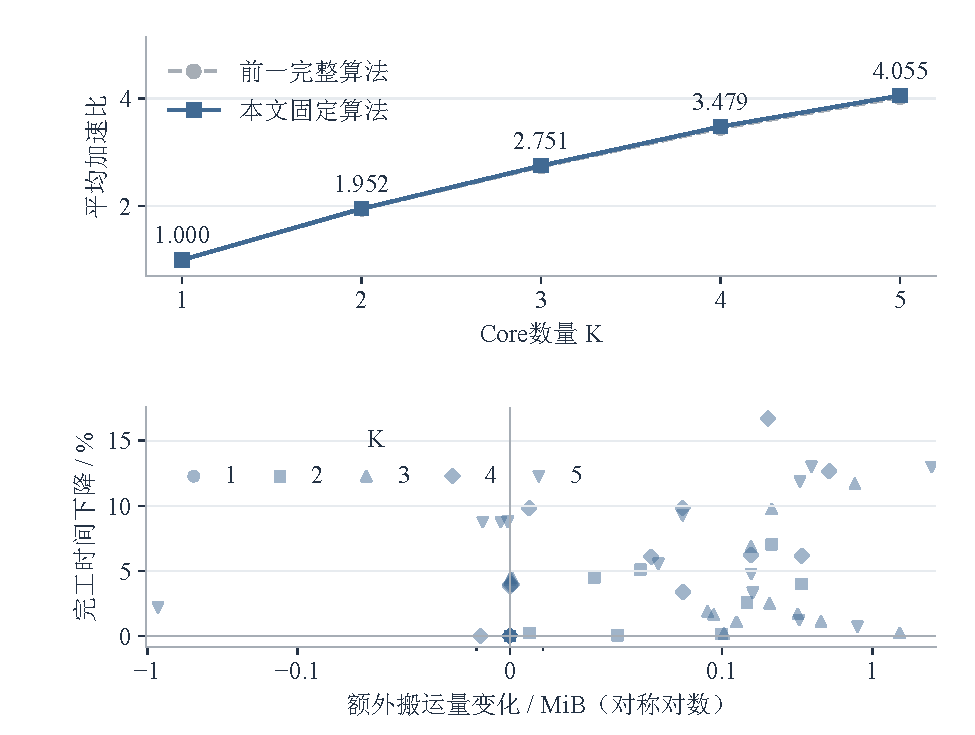
\includegraphics[width=\linewidth,height=.84\textheight,keepaspectratio]{figures/paper-v2/fig-p1-results.pdf}
\caption{问题一的完整版本比较。上：每个核心数量的 100 图平均加速比；下：全部500种图与核心数量组合的时间与搬运量配对变化。核心数量用点形区分，横轴采用对称对数。}
\label{fig:p1-results}
\end{figure}

\subsection{典型案例微架构执行时序分析（Case 026）}

为了在微架构时钟周期与硬件流水线级别理解分支援助细化的执行特征，我们选取典型用例 \texttt{case\_026}（5 Cores 配置）进行结构与时序分析。

该用例在分支援助重分配前后的宏观指标对比体现如下：

\begin{itemize}
\tightlist
\item
  \textbf{细化前父方案}：由 \texttt{\seqsplit{structural\_refine}} 生成 5 个 Task。官方 E0 仿真评测的 Makespan 为 44,114 cycles，调度产生的额外 DDR 搬运量为 211,680 字节；
\item
  \textbf{细化后采纳方案}：经 \texttt{branch\_aid} 调整后扩展为 7 个 Task。官方 E0 仿真评测的 Makespan 缩短为 42,014 cycles，调度产生的额外 DDR 搬运量为 375,532 字节。
\end{itemize}

方案调整使得该用例的全局完成时间降低了 2,100 cycles（完成时间降幅为 4.76\%），其代价是额外 DDR 数据搬运量增加了 163,852 字节。

图 \ref{fig:p1-overlap} 绘制了基于官方模拟事件生成的执行时间线。从图中可以观察到微架构层面的负载分布与流水线事件：

\begin{enumerate}
\def\labelenumi{\arabic{enumi}.}
\tightlist
\item
  \textbf{初始负载分析}：在原始划分中，波次 0 内部的算子集中在 Core 0 上的单个 Task 中，其在向量流水线上的预估计算工作量代理峰值为 40,824 cycles；
\item
  \textbf{分支剥离与工作量调整}：算法识别出 Task 内部由算子 714、716、722 组成的独立向量分支 \(X\)，并将其剥离为子图 6 迁移至 Core 1 上执行；原 Core 0 则保留分支 \(Y\)（子图 0，包含算子 710、712、720）与汇合部分 \(J\)（子图 5，包含算子 724、726）。在调度序列中，Core 1 排定优先执行支路 \(X\)，各核心各流水线的预估计算工作量代理峰值由 40,824 cycles 降至 37,569 cycles；
\item
  \textbf{完成时间表现}：跨核迁移使得算子 722 生成的中间张量需要通过 DDR 读写传递给 Core 0 上的汇合算子 724，额外 DDR 搬运量增加了 163,852 字节。在官方模拟推进下，方案整体 Makespan 呈现出 2,100 cycles 的净缩减；由于微架构事件中并发计算、访存排队与同步等待相互交织，此处 2,100 cycles 的改善反映了方案调整后的整体模拟结果，而不宜在缺乏消融隔离的情况下直接归因于单一维度的因果分摊。
\end{enumerate}

\begin{figure}[!htbp]\centering
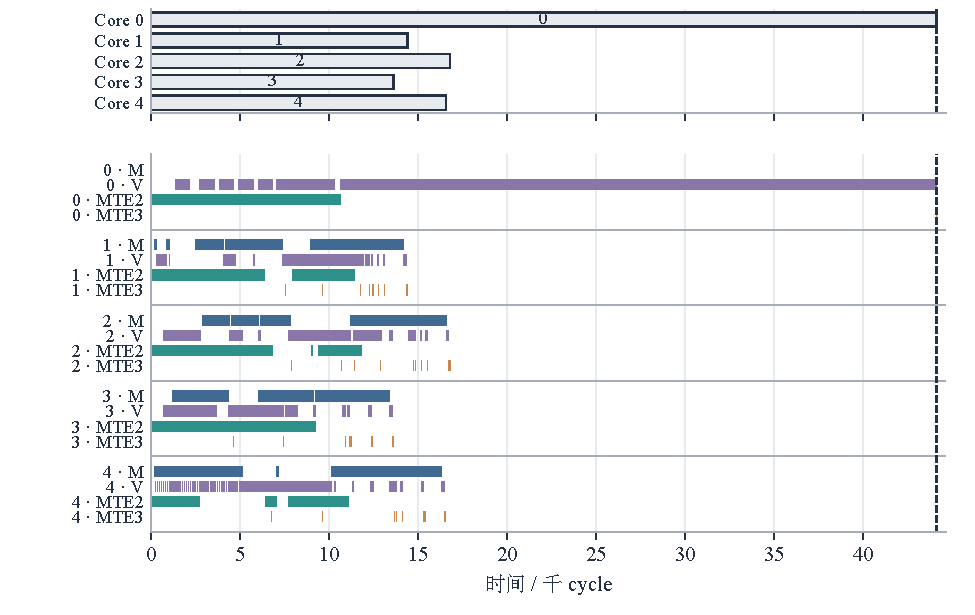
\includegraphics[width=\linewidth]{figures/paper-v2/fig-p1-overlap-old.pdf}
\par\vspace{4pt}
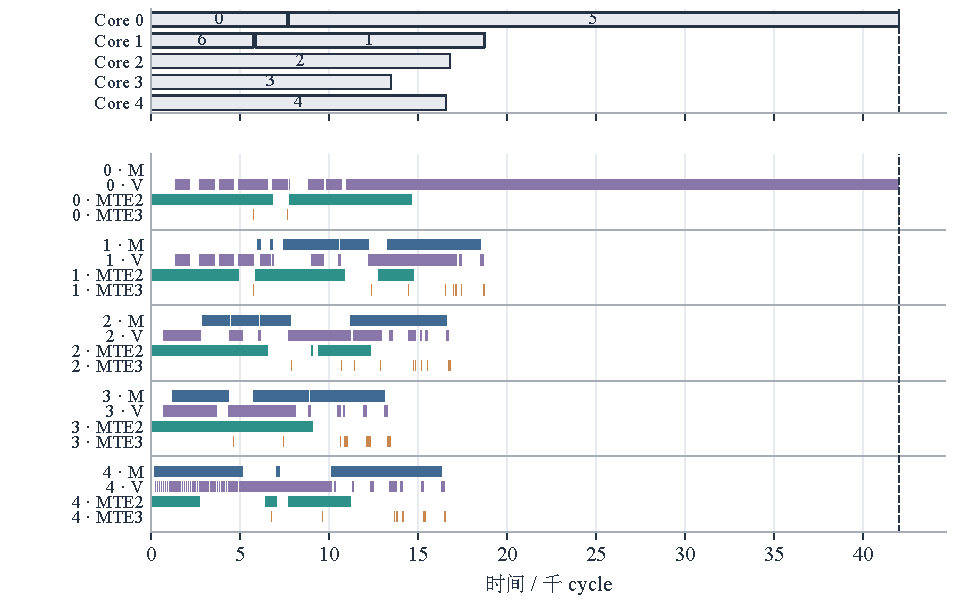
\includegraphics[width=\linewidth]{figures/paper-v2/fig-p1-overlap-new.pdf}
\caption{case\_026、5个核心 两种切分的执行时间线。上：修改前方案，$M=44{,}114$ cycles，额外搬运211,680 B；下：分支重新分配后，$M=42{,}014$ cycles，额外搬运375,532 B。每组分别显示Task持续区间及四条Pipe的操作区间，横轴范围相同，数据来自官方模拟事件。}
\label{fig:p1-overlap}
\end{figure}

该案例反映了多核心硬件调度中的典型权衡：通信量的局部上升并不必然导致整体性能劣化；当多核心并行推进缩短排队的效果超过数据搬运与同步时延时，即可在官方模拟中获得全局完成时间的改善。


\section{问题二：联合安排计算位置与数据搬运}

\subsection{同一核心内的数据复用与存储权衡}

在问题二的系统设定中，被分配到同一个计算核心的全部子图在底层编译时被合并为一个整体硬件执行任务（Task）。这一微架构语义的变化带来了根本性的数据流动革新：在同一核心内部，先前执行的子图算子所生成的数据张量可以直接保留在该核心的片上私有缓存（L1 Buffer 与 Unified Buffer，UB）中，供后继子图中的算子直接读取复用，无需再经由外部主存（DDR）进行持久化中转。

然而，若数据生成算子与数据消费算子被分配至不同的计算核心，则数据依然必须通过跨核心通信链路传递：由源核心执行 \texttt{COPY\_OUT} 将数据写入 DDR，再由目标核心执行 \texttt{COPY\_IN} 将数据读入本地缓存。在硬件时序上，目标核心的读取操作必须在源核心写出操作彻底完成 500 cycles 之后方可启动。在此执行模型下，即使在方案提交文件（\texttt{\seqsplit{node\_to\_subgraph}}）中将每个计算算子单独划分为一个子图，也不会在硬件底层为每个算子生成孤立的物理 Task，子图序列仅用于指示底层编译器在各核心内部排定算子的先后执行次序。

同核心任务合并显著加深了算子分配与调度顺序之间的耦合关联，并引出了新的微架构存储权衡：

\begin{enumerate}
\def\labelenumi{\arabic{enumi}.}
\tightlist
\item
  \textbf{缓存复用收益}：将具有密集张量消费关系的算子聚集至同一计算核心，可彻底消除跨核 DDR 往返读写流量以及 500 cycles 的跨核同步等待；
\item
  \textbf{片上存储驻留压力与溢出代价}：若过度追求局部复用而将算子集中，或者消费同一张量的多个算子在执行时序上相距过远，该中间张量就必须在片上私有缓存中维持长时间的驻留生命周期。当片上缓存容量不足以容纳活跃数据峰值时，官方编译系统将在其内部流程的第二阶段（Step 2）强制插入溢出换出与换入操作（spill），从而在执行阶段产生意料之外的二次 DDR 读写开销；
\item
  \textbf{空间复用与时间并行的冲突}：将数据消费算子分散至其他核心虽会引入边界数据搬运，但能有效利用多核计算资源展开并行计算，并释放本地片上存储压力。
\end{enumerate}

因此，私有缓存容量限制与 Step 2 溢出（spill）深刻影响着系统的实际数据搬运总量。多核心调度算法必须在控制跨核数据流动的同时，防止片上工作量与存储过度聚集。

\subsection{利用执行资源空闲区间安排计算}

为了在调度构建阶段兼顾计算流水线的利用率，算法设计了基于空闲时间区间（gap intervals）的拓扑编排机制。该机制实时维护各计算核心在输入计算图中实际出现的各类执行流水线（如 \texttt{PIPE\_M}、\texttt{PIPE\_V} 等）上已排定算子的占用时间区间集合。

在处理计算链时，算法沿链内依赖拓扑顺序依次为各算子寻找可行空闲区间。设待排定算子 \(v\) 的计算时长为 \(d_v = \max(1, \text{cycles}_v)\)，其在当前部分调度下的估计最早数据就绪时刻为 \(r_v\)。记 \(\mathcal{I}_{k, p_v}\) 为核心 \(k\) 上对应流水线 \(p_v\) 已占用时间区间的并集。算法在满足数据依赖约束的前提下，在时间轴上寻找最早满足互不重叠条件的空闲时间窗口，选取最早的可行启动时刻 \(s_v\)：

\begin{equation}
s_v \ge r_v, \qquad [s_v, s_v + d_v) \cap \mathcal{I}_{k, p_v} = \emptyset.
\end{equation}

时间区间采用左闭右开表示，允许后继算子在前序算子完成的时钟周期无缝衔接。在多支路汇聚节点处，为了避免局部贪心导致单侧支路过度滞后，算法在汇合算子两侧至多联合枚举 \(K^2\) 种核心指派组合，综合评估不同核心搭配下的完成时刻。

需要强调的是，上述空闲区间计算仅为引导候选方案构造的启发式时间代理（proxy heuristic），其并未模拟底层 DDR 访问仲裁、总线带宽争用以及复杂的片上存储空间动态分配。因此，估计时刻 \(s_v\) 既不构成全局 Makespan 的数学上界，亦不构成理论下界。方案的物理执行时刻最终由官方离散事件仿真器推进确定。

同一个核心保留数据与在不同核心之间复制数据的区别见图 \ref{fig:progression}。后续按这个区别计算边界复制量。

\subsection{基于超图连接度模型的复制量度量}

在普通图模型中，传统图割算法将数据流动简化为边权切分，无法准确刻画``一对多''数据复用的真实开销。

考察一个典型的复用场景：算子 \(u\) 生成大小为 8 B 的张量 \(t\)，算子 \(v_1\) 与 \(v_2\) 均读取 \(t\)。在硬件执行层面上，若将读取算子 \(v_1\) 与 \(v_2\) 分配至同一个远端核心，该核心只需从 DDR 读入一次 8 B 数据即可供两个算子共同使用（对应源核心一次 \texttt{COPY\_OUT} 与目标核心一次 \texttt{COPY\_IN}，共产生 16 B 边界流量）；若仅将 \(v_1\) 移回 \(u\) 所在核心，由于 \(v_2\) 仍驻留在远端，该远端核心依然需要完整搬入该张量，边界复制量依然维持 16 B；只有当 \(v_1\) 与 \(v_2\) 均被移回 \(u\) 所在核心时，跨核数据传递需求才彻底消失，相关边界复制量降为 0 B。在不同的核心分配下，该张量引发的边界复制量分别为 16 B、16 B 与 0 B。这种非线性特征表明，边的割断无法等价于数据复制。

为精确刻画多算子共同使用同一数据的共享边界，本文引入\textbf{超图}（hypergraph）模型 \(\mathcal{H} = (V, \mathcal{E})\)。超图由算子顶点集 \(V\) 与\textbf{超边}（hyperedge）集合 \(\mathcal{E}\) 构成，每条超边连接任意非空的顶点子集（允许包含单个顶点）\cite{ref5}。在并行计算与数据划分领域，利用超图连接度模型刻画多处理器间的通信开销是经典的方法论基础\cite{ref3}。超图仅表示算子间的数据关联关系，不指示计算先后顺序；原计算图的有向拓扑依赖另行独立维护。

\subsubsection{模型定义与适用领域}

超图模型严格适用于如下计算图领域：

\begin{enumerate}
\def\labelenumi{\arabic{enumi}.}
\tightlist
\item
  顶点集 \(V\) 完整包含除跨边界核外搬运操作 \texttt{COPY\_IN} 与 \texttt{COPY\_OUT} 之外的全部原始待调度算子；
\item
  严格拒绝逻辑张量别名（\texttt{\seqsplit{logical\_tid}}），每个物理张量具有唯一的物理生成算子，张量大小 \(b_t\) 为非负整数；
\item
  直接算子间依赖边（direct op-op edges）亦纳入模型统一处理。
\end{enumerate}

\subsubsection{超边构成与权值定义}

对于计算图中的数据传递关系，超边集 \(\mathcal{E}\) 与固定常数项 \(C\) 按如下规则精确构建：

\begin{enumerate}
\def\labelenumi{\arabic{enumi}.}
\tightlist
\item
  \textbf{外部输入张量}：该张量在计算图内无生成算子，其超边引脚集合仅包含所有读取该输入的算子子集 \(\operatorname{cs}\)。每增加一个需要该输入的核心，需额外从 DDR 搬入 \(b_t\) 字节，故超边权重赋值为 \(w_e = b_t\)；其首次读入的基础复制量计入全局常数项 \(C\)；
\item
  \textbf{中间数据张量}：超边引脚集合包含其生成算子以及全部读取该张量的计算算子 \(\operatorname{cs} \cup \{\operatorname{producer}\}\)。依官方冻结评测编译语义，跨核心访问时涉及源核心写出外存与目标核心读入本地的一对操作，故超边权重赋值为 \(w_e = 2b_t\)（硬件常数严格依据源码，不作未经证实的广播假设）；若该张量同时被外部 \texttt{COPY\_OUT} 消费或在图内无后继消费者，其写出外存的固定开销 \(b_t\) 累加至常数项 \(C\)；
\item
  \textbf{直接算子依赖边}：引脚集合为 \(\{u, v\}\)，权重赋值为 \(w_e = 2 \times \operatorname{data\_size}(e)\)；
\item
  引脚集合为空或权重为零的超边被直接丢弃。
\end{enumerate}

\subsubsection{预 Step 2 原始复制字节数公式}

给定算子到计算核心的指派映射 \(a: V \to \{0, 1, \dots, K-1\}\)，定义 \(\lambda_e(a)\) 为超边 \(e\) 中全部算子所跨越的不同核心数量（无量纲整数）。在官方评测程序第二阶段（Step 2）插入缓存溢出换入换出之前，方案的\textbf{预 Step 2 原始复制字节数}（pre-Step2 original COPY bytes）精确满足：

\begin{equation}
D_{\mathrm{pre2}}(a) = C + \sum_{e \in \mathcal{E}} w_e \bigl(\lambda_e(a) - 1\bigr).
\end{equation}

其中，\(D_{\mathrm{pre2}}\)、\(C\) 与 \(w_e\) 的单位均为字节（B）。当一条超边的所有相关算子均指派给同一核心时，\(\lambda_e(a) = 1\)，对求和式的贡献为 0；每向一个新核心延伸，均线性增加 \(w_e\) 字节。该指标严格度量了划分切口在未发生缓存溢出时的固有通信量，并不等同于最终包含溢出换入换出的额外 DDR 搬运量（\texttt{\seqsplit{added\_copy\_bytes}}），亦不代表 Makespan。

\begin{figure}[!htbp]
\centering
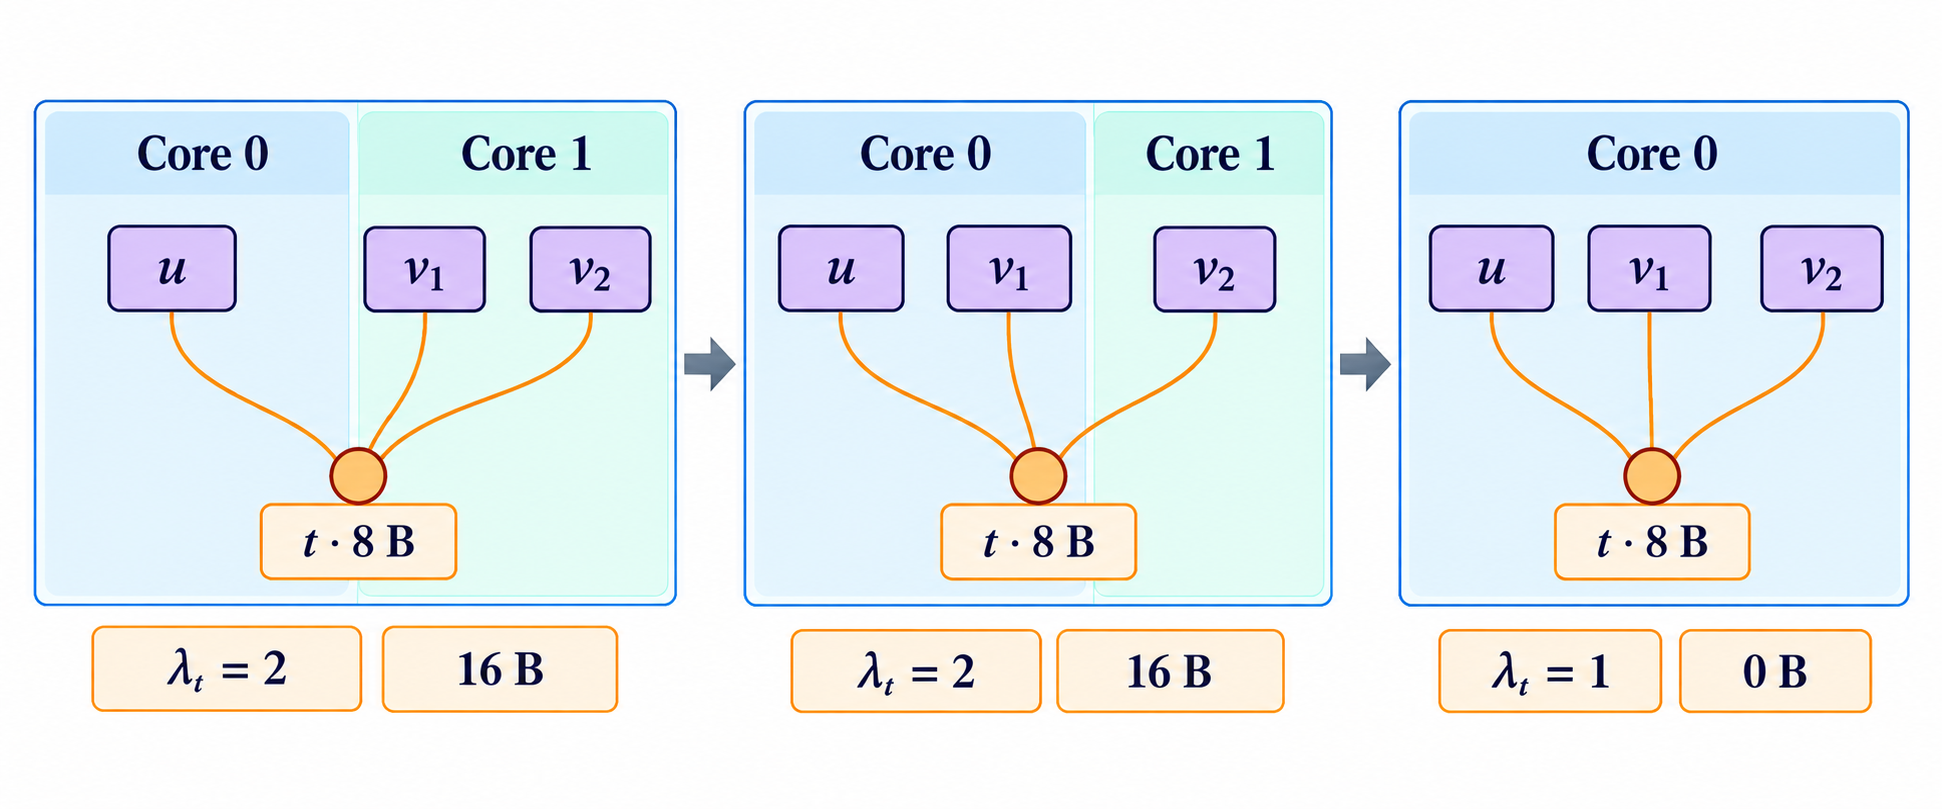
\includegraphics[width=\linewidth,height=.84\textheight,keepaspectratio]{figures/fig-hypercut-v2.png}
\caption{同一张量的计算操作分配。图中 $u$ 生成 $t$，$v_1, v_2$ 读取 $t$；$\lambda_t$ 表示这三个操作所在的不同核心数量。16 B、16 B、0 B 仅统计该张量的边界复制，线条只表示集合关联。}
\label{fig:hypercut}
\end{figure}

\subsubsection{分组移动的增量更新法则}

当算法将一组算子 \(A \subset V\) 从源核心 \(s\) 整体迁移至目标核心 \(t\)（\(s \ne t\)）时，要求 \(A\) 中的所有算子在迁移前必须处于同一源核心 \(s\)（不支持跨源核心的混合分组移动）。

对于任意与 \(A\) 相交的超边 \(e\)，令 \(n_{e, s}\) 与 \(n_{e, t}\) 分别为迁移前超边 \(e\) 在源核心与目标核心上的引脚数量，令 \(m_e = |e \cap A|\) 为超边 \(e\) 中被迁移的引脚数。超边 \(e\) 的复制字节变化量 \(\Delta_e\) 严格满足：

\begin{equation}
\Delta_e = w_e \left( \mathbf{1}\{n_{e, t} = 0\} - \mathbf{1}\{n_{e, s} = m_e\} \right).
\end{equation}

其中 \(\mathbf{1}\{\cdot\}\) 为指示函数。若目标核心原先未包含该超边算子，则新增一个跨核副本（增加 \(w_e\)）；若源核心所包含的该超边算子被全部移走，则彻底消除源核心的副本需求（减少 \(w_e\)）。总变化量为所有相交超边 \(\Delta_e\) 的代数和。在连续执行多次分组调整时，算法只需增量维护各超边在各核心的引脚计数 \(n_{e, k}\)。

\subsection{计算工作量约束下的局部最小割方法}

为了优化上述超图连接度目标，算法在空闲区间构造方案的基础上，选取两个核心 \(a, b\) 以及最多 16 条前后相连的计算链（chain，总数 \(w \le 16\)）作为局部调整区域。所选区域之外的全部算子核心分配保持锁定，区域内的各条计算链在核心 \(a\) 与 \(b\) 之间决策归属。

\subsubsection{辅助网络构建与精确映射}

在固定范围外算子后，最小化二核心之间的超图连接度可通过构建有向辅助网络转化为源汇最小割（minimum source-target cut）问题。利用有向辅助网络将特定超边切分代价转化为源汇割模型在超图割文献中已有理论研究\cite{ref8}；本实现针对固定引脚与二核心指派给出具体的 OR 辅助网络映射与代数证明，该构造并不推广至任意次模分割函数，亦不推出带容量约束的全局 Makespan 最优。

设源点对应核心 \(a\)（割的源侧为分配至 \(a\) 的单元），汇点对应核心 \(b\)（割的汇侧为分配至 \(b\) 的单元）。对于每条超边 \(e\)，其在局部自由可移动单元集合之外的固定引脚所归属的核心集合记为 \(\operatorname{fixed\_cores}\)（注意：\(\operatorname{fixed\_cores}\) 可能包含核心 \(a\)、核心 \(b\)，亦可能包含其他计算核心，且可能为空集）。

算法无条件累加所有超边的固定项至基准常数：

\begin{equation}
\text{offset} = \sum_{e \in \mathcal{E}} w_e (|\operatorname{fixed\_cores}| - 1).
\end{equation}

特别地，当某条超边在调整区域外无任何固定引脚时，\(\operatorname{fixed\_cores} = \emptyset\)，其贡献项为 \(-w_e\)。

网络弧权与辅助节点按如下规则构造：

\begin{enumerate}
\def\labelenumi{\arabic{enumi}.}
\tightlist
\item
  \textbf{有限弧权和与无穷容量设定}： \begin{equation}
\text{finite\_sum} = \sum_{e \in \mathcal{E}} w_e \left( \mathbf{1}\{a \notin \operatorname{fixed\_cores}\} + \mathbf{1}\{b \notin \operatorname{fixed\_cores}\} \right), \quad \infty = \text{finite\_sum} + 1.
\end{equation}
\item
  \textbf{核心 \(a\) 覆盖代价辅助节点 \(aux_a\)}：若 \(a \notin \operatorname{fixed\_cores}\)，建立辅助节点 \(aux_a\)。从超边 \(e\) 内的各个自由计算链节点向 \(aux_a\) 连接容量为 \(\infty\) 的有向弧，并从 \(aux_a\) 向汇点连接容量为 \(w_e\) 的有向弧。若该超边有任意一条链被分配给核心 \(a\)（落入源侧集合 \(S\)），最小割必须切断容量为 \(w_e\) 的弧；
\item
  \textbf{核心 \(b\) 覆盖代价辅助节点 \(aux_b\)}：若 \(b \notin \operatorname{fixed\_cores}\)，建立辅助节点 \(aux_b\)。从源点向 \(aux_b\) 连接容量为 \(w_e\) 的有向弧，并从 \(aux_b\) 向该超边的各个自由计算链节点连接容量为 \(\infty\) 的有向弧。若有任意一条链被分配给核心 \(b\)（落入汇侧集合 \(T\)），最小割必须切断容量为 \(w_e\) 的弧；
\item
  \textbf{锚定弧（anchors）}：若某计算链单元 \(u\) 被强制锁定在核心 \(a\)，则添加容量为 \(\infty\) 的源点指向 \(u\) 的弧；若锁定在核心 \(b\)，则添加 \(u\) 指向汇点的 \(\infty\) 弧。
\end{enumerate}

该辅助网络的最大流值 \(F\) 与局部超图连接度严格满足恒等关系：\(\operatorname{Cost} = \text{offset} + F\)。

以空固定集合（\(\operatorname{fixed\_cores} = \emptyset\)）的情形为例：此时超边所有引脚均为局部自由单元。若所有引脚最终均被划入核心 \(a\)，该超边仅触及 1 个核心，实际连接度贡献为 \(w_e (1 - 1) = 0\)。在辅助网络中，因 \(a \notin \operatorname{fixed\_cores}\)，引脚落入源侧切断了 \(aux_a \to \mathrm{sink}\) 的弧，贡献流值 \(w_e\)；而因无引脚落入汇侧，\(b\) 侧未贡献流值。此时网络流值 \(F = w_e\)。结合固定基准常数 \(\text{offset} = -w_e\)，二者相加恰好为 \(-w_e + w_e = 0\)，与真实超图连接度严格相等。若引脚同时跨越 \(a\) 与 \(b\)，两项 OR 边均被切断，流值为 \(2w_e\)，总和为 \(-w_e + 2w_e = w_e = w_e (2 - 1)\)，同样严格相等。因此，Dinic 算法\cite{ref9}求得的割精确给出了在当前锁定引脚与锚定约束下，局部二核心连接度目标的最优解。

\subsubsection{计算工作量上限保护（Load Guard）}

单纯追求复制字节最小化可能导致最小割将绝大部分计算集中指派至单一核心，诱发严重的计算延迟倾斜。为此，算法引入了受工作量保护的闭环最小割算法（\texttt{\seqsplit{load\_guarded\_cut}}）。

算法统计各核心在各计算流水线上的初始累计时长，取全核心初始工作量的峰值作为各流水线的硬性工作量上限（caps）。若求解最小割后得到的分配方案导致某个核心在某条流水线上的总工作量超出了预设上限，算法将在导致超额的迁入链中，选出在该流水线上耗时最长的一条链，将其锚定回初始分配状态，并重新求解辅助网络的最小割。

\textbf{命题5.1（局部复制量与工作量保护性质）。} 若初始分配满足流水线工作量上限，且每次锚定均将单元固定回其初始核心，则 \texttt{\seqsplit{load\_guarded\_cut}} 算法在至多 \(w + 1\) 次最大流求解内必终止，且终止时所得方案的局部预 Step 2 复制量 \(D_{\mathrm{pre2}}\) 绝不大于初始分配，且各流水线工作量均不超过上限。

\begin{proof} 初始分配始终完全满足工作量上限约束。由于每次锚定均与初始分配一致，初始分配在每一次增加锚定约束后的辅助网络中始终构成一个合法的割。根据最小割的最优性，求得的最小割代价必不高于初始分配的代价值。由于局部自由链的总数为 \(w\)（\(w \le 16\)），若每次迭代均发生工作量超限，每次至少有一条链被永久锁定回原位置。在最坏情况下，经过至多 \(w\) 次锁定后，全部流动链均被重置回初始分配，此时工作量超限自然消除。因此，算法必在至多 \(w + 1\) 次求解内终止，且终止解的局部复制字节数不高于原方案。 \end{proof}

需要明确指出的是，命题 5.1 证明的仅是在给定的局部二核心区域及锚定启发过程下预 Step 2 复制量不增加且流水线工作量不超限。流水线工作量上限是通过迭代式的启发式锚定进行防护，而非单次带约束规划的全局最优解；该机制\textbf{并不保证}片上缓存不发生溢出（spill），\textbf{并不保证}全局 Makespan 一定缩短，亦非全图范围的多核全局最优解。算法仍须依赖最终的离散事件仿真来进行综合裁决。

\subsection{完整算法流程与候选方案选优}

\textbf{算法2：问题二联合切分与多核调度算法（P2 Solver）。}

\begin{lstlisting}[style=gmcmappendix,language={}]
输入：原始计算图 G、核心数 K、官方硬件配置 config。
输出：合法的切分与调度方案 P = (node_to_subgraph, core_schedules)。
1. 调用自适应装箱模块生成基础基线方案 baseline（P0）；
2. 尝试利用流水线空闲区间重排计算顺序，构造 gap 候选方案（P1）；若遇到不支持的拓扑结构或构造异常，直接安全回退至 baseline；
3. 以 gap 方案为基准，提取最多 16 条链构建局部超图，执行受负载保护的二核心最小割（gap_hyperrefine）；
4. 统计细化前后的预 Step 2 复制字节数：
     若 after_original_copy_bytes < before_original_copy_bytes（实现严格减少）：
         调用重定时模块（gap_retime）重新排定执行顺序，生成 hypergap 候选方案（P2）；
     若复制字节未严格减少：
         跳过 hypergap 构造，严格保留未经修改的原 gap 方案参与后续比选；
5. 汇总互不相同的完整候选方案（在 baseline, gap, hypergap 中至多保留 3 份不同方案）；
6. 严格按构造先后顺序，向底层在线评测适配器提交评分请求（至多 3 次评分请求）。单次评测必须成功返回原生评测且状态正常（route == 'native' 且 status == 'ok'）的得分向量方用于比较；若评测返回非原生路由（如记录的 e0_fallback）或评测抛出异常，适配器将拒绝采纳该结果并抛出错误，外层控制器捕获异常后安全终止本轮选优，直接返回保底的 baseline 方案；
7. 依据有效原生评测反馈的目标向量 (Makespan, added_copy_bytes) 按字典序选优，输出综合表现最佳的合法方案。
\end{lstlisting}

在该体系中，\texttt{baseline}、\texttt{gap} 与 \texttt{hypergap} 代表本求解流程中生成的不同方案构型。预 Step 2 复制字节的减少仅作为触发 \texttt{gap\_retime} 的控制门槛，并不用于提前剪除未修改的 \texttt{gap} 方案。在线评测上限严格冻结为 3 次评分请求，评测异常时统一安全回退至 baseline。

\subsection{全量实验评测与结果分析}

本文算法在官方提供的 100 张全量基准计算图、涵盖 1 至 5 核心的全部 500 种测试组合上进行了完整的端到端求解与评测，所有方案均顺利通过官方合法性校验并正常推进完成。测试结果依据 \texttt{\seqsplit{paper/manuscript-v1/data/all-results.csv}} 以及固定评测数据资产（\texttt{\seqsplit{p2-audit.json.gz}}，对应求解器 Commit \texttt{c66559a}）进行了精确复核。

下表分别列出题目规定的官方基准平均加速比，以及使用算法输出方案计算的平均加速比。

\begin{table}[!htbp]\centering\small

\begin{tabularx}{\linewidth}{@{}Xrrrrr@{}}\toprule
核心数量 & 1 & 2 & 3 & 4 & 5 \\
\midrule
官方口径平均加速比 & 1.0000 & 2.3167 & 3.2356 & 3.9711 & 4.5498 \\
优化方案 $\operatorname{mean}(B/M)$ & 1.2061 & 2.3167 & 3.2356 & 3.9711 & 4.5498 \\
改善/持平/退化 & 59/41/0 & 64/36/0 & 54/46/0 & 49/51/0 & 42/58/0 \\
求解时间均值 / s & 2.613 & 3.863 & 4.251 & 4.498 & 4.921 \\
\bottomrule\end{tabularx}\end{table}

如表中数据所示：

\begin{enumerate}
\def\labelenumi{\arabic{enumi}.}
\tightlist
\item
  \textbf{多核加速比与单核比值解析}：在 2 至 5 核场景下，官方主口径平均加速比分别达到 2.3167、3.2356、3.9711 以及 4.5498。在单核场景下，算法输出方案相比官方单核基线取得了 1.2061 的 \(B/M\) 比值（该比值超出基线 1.0 的幅度为 20.61\%，反映算法输出的单核方案 Makespan 优于官方基准，不代表完成时间单调下降 20.61\%）。表中两行在单核场景下的分子 \(B\) 均严格采用官方单核基准 Makespan，差异源于分母方案不同（官方主口径行以官方基准方案自身为分母，比值为 1.0000；第二行以算法实际输出方案为分母，比值平均为 1.2061）。与前一固定版本相比，全量 500 个测试网格中共有 268 个用例缩短了 Makespan，232 个用例持平，实现零退化（degrade = 0）；全网格共有 69 张计算图在至少一个核心数下取得了性能突破；
\item
  \textbf{通信流量与多核权衡}：全量 500 个用例的额外 DDR 搬运总量从基准版本的 3,043,860,416 字节上升至 4,159,738,560 字节（增幅为 36.66\%）。深入分析 500 个用例的性能变动分布：共有 55 个用例实现了执行时间与搬运量双重下降；199 个用例执行时间显著缩短但搬运量有所增加；14 个用例执行时间缩短而搬运量持平；其余 232 个用例两项指标均保持不变。该分布反映了算法以主目标（Makespan）优先的选优取向：在版本迭代中观察到了执行时间显著下降与额外搬运量增加相伴随的成对数值变动，此处仅客观记录前后版本对比的数据呈现，不作未经独立消融隔离的因果机制归因；
\item
  \textbf{评测调用账与计算效率}：在全量 500 次独立求解过程中，累计发起 1131 次在线 native E2 评测请求，全部成功返回原生结果，未触发任何向 E0 的异常回退。独立外部 E0 仿真复验亦全部顺利完成。采用最近秩次法（nearest-rank，取第 \(\lceil 0.95n \rceil\) 位），全量 500 个用例的求解程序物理墙钟时间均值为 4.029 秒，95\% 分位数（第 475 位）为 18.841 秒，最大求解时间为 40.187 秒；独立的外部 E0 仿真耗时均值为 1.410 秒，95\% 分位数（第 475 位）为 6.592 秒，最大值为 13.980 秒。全网格耗时稳定在建议的高效时间范围之内。
\end{enumerate}

\begin{figure}[!htbp]
\centering
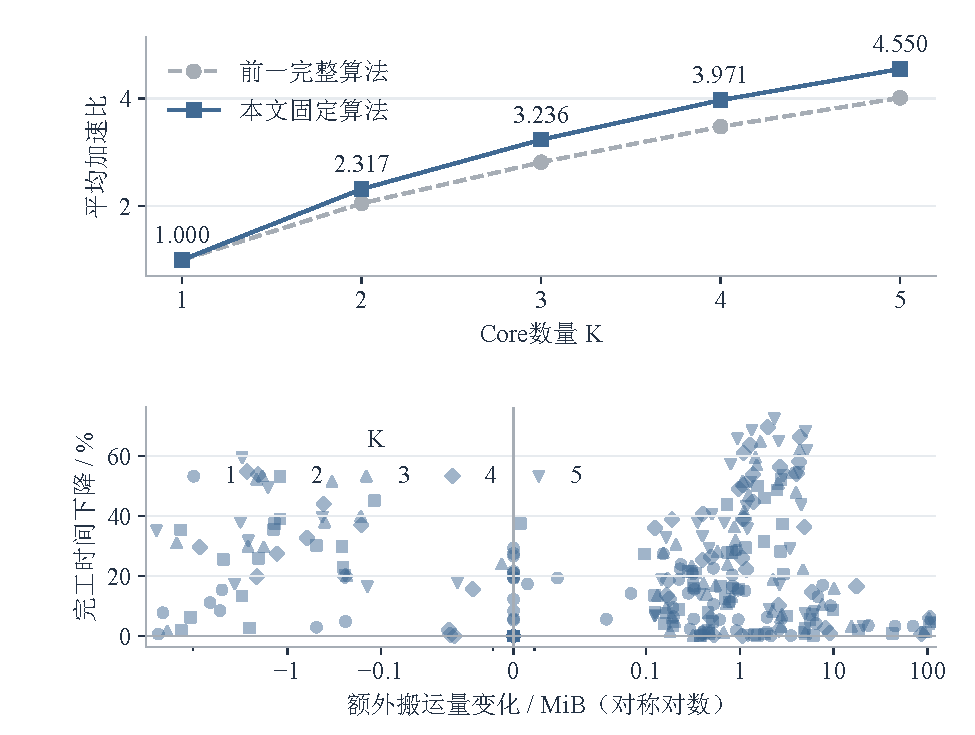
\includegraphics[width=\linewidth,height=.84\textheight,keepaspectratio]{figures/paper-v2/fig-p2-results.pdf}
\caption{问题二的完整版本比较。上：按题目要求计算的平均加速比；下：500种组合配对结果。部分时间改善伴随额外搬运增加，两项指标分别报告。}
\label{fig:p2-results}
\end{figure}

\subsection{减少搬运量反而增加完成时间的反例（C04）}

为了严格检验``仅按片上容量和搬运量构造调度方案''是否存在固有缺陷，前期研发实验针对另一种固定构造策略（代码代号 C04）对六个预先指定的 5 核心用例进行了对比评测。

在该对照实验中，C04 生成的六份方案在格式与时序上完全合法，且经官方 Step 2 编译确认未插入任何由于容量超限导致的缓存换入换出（spill 为 0）。然而，其最终 Makespan 全面劣于本文主算法，对比数据如下表所示：

{\def\LTcaptype{table} % do not increment counter
\begin{table}[!htbp]\centering\small
\begin{tabular}{@{}
  >{\raggedright\arraybackslash}p{(\linewidth - 6\tabcolsep) * \real{0.2000}}
  >{\raggedleft\arraybackslash}p{(\linewidth - 6\tabcolsep) * \real{0.2667}}
  >{\raggedleft\arraybackslash}p{(\linewidth - 6\tabcolsep) * \real{0.2667}}
  >{\raggedleft\arraybackslash}p{(\linewidth - 6\tabcolsep) * \real{0.2667}}@{}}
\toprule\noalign{}
\begin{minipage}[b]{\linewidth}\raggedright
用例名称
\end{minipage} & \begin{minipage}[b]{\linewidth}\raggedleft
本文主算法 / cycles
\end{minipage} & \begin{minipage}[b]{\linewidth}\raggedleft
C04 对照方案 / cycles
\end{minipage} & \begin{minipage}[b]{\linewidth}\raggedleft
相对变慢幅度
\end{minipage} \\
\midrule\noalign{}


case\_005 & 33,515 & 38,209 & +14.01\% \\
case\_016 & 2,091,375 & 2,399,125 & +14.72\% \\
case\_019 & 16,247 & 28,514 & +75.50\% \\
case\_025 & 942,938 & 975,658 & +3.47\% \\
case\_039 & 449,653 & 494,942 & +10.07\% \\
case\_075 & 343,930 & 452,120 & +31.46\% \\
\bottomrule\end{tabular}
\end{table}
}

尤其在 \texttt{case\_019}、\texttt{case\_039} 与 \texttt{case\_075} 中，C04 方案的边界 COPY 字节数明显低于本文主算法，但其执行完成时间却出现了大幅退化（在 \texttt{case\_019} 中变慢达 75.50\%）。

图 \ref{fig:p2-counterexample} 给出了 \texttt{case\_019} 在官方离散事件仿真下的执行时序对比。数据显示，C04 方案的边界 COPY 字节数显著低于主算法，且无片上容量不足引发的 Step 2 缓存换入换出（spill 为 0），但其最终执行完成时间显著增加（Makespan 变大 75.50\%）。关于硬件资源利用与等待时长的具体归因，仍待进一步的事件分类统计验证。

\begin{figure}[!htbp]\centering
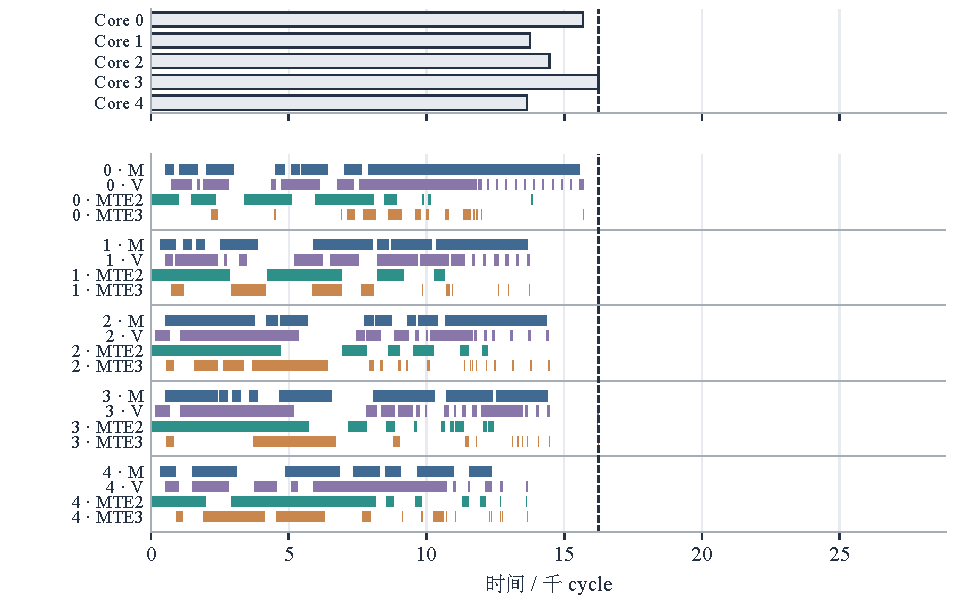
\includegraphics[width=\linewidth]{figures/paper-v2/fig-p2-counterexample-control.pdf}
\par\vspace{4pt}
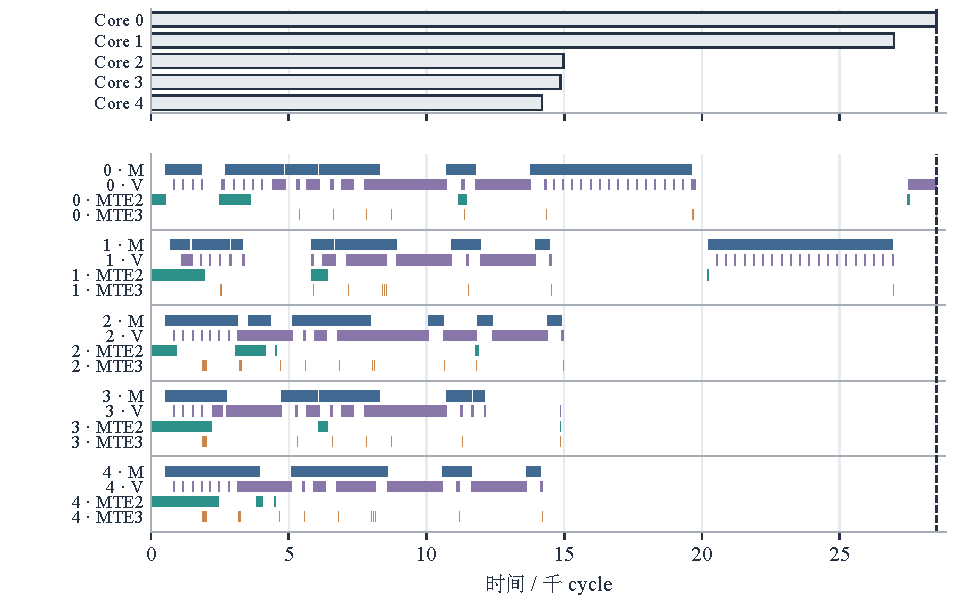
\includegraphics[width=\linewidth]{figures/paper-v2/fig-p2-counterexample-c04.pdf}
\caption{case\_019、5个核心的官方模拟的执行时间线。上：主算法，$M=16{,}247$ cycles；下：C04，$M=28{,}514$ cycles。每组分别显示Task和四条Pipe，共用横轴范围。C04的搬运量较少，且没有容量不足引起的缓存换入换出，但完成时间更长。}
\label{fig:p2-counterexample}
\end{figure}

上述限定反例表明：单纯优化静态通信数据量并不能直接保证任务执行时间的缩短。

\subsection{计算复杂度与算法护栏分析}

算法在求解过程中将各阶段计算开销解耦：

\begin{enumerate}
\def\labelenumi{\arabic{enumi}.}
\tightlist
\item
  \textbf{图拓扑识别与链分解}：构建算子依赖拓扑并提取独立计算链；
\item
  \textbf{空闲区间扫描}：在候选构造过程中，算子插入需遍历维护的时间段集合，设累计扫描的时间段总数为 \(Q\)；
\item
  \textbf{汇聚点配对检查}：在多支路汇合节点处枚举核心指派组合，涉及至多 \(K^2\) 种局部搭配与对应的排定开销；
\item
  \textbf{局部超图最小割与保护循环}：设共优化 \(R\) 个局部区域。第 \(j\) 个区域的辅助网络包含 \(n_j\) 个节点与 \(m_j\) 条弧，内部包含 \(w_j \le 16\) 条自由链。采用 Dinic 算法\cite{ref9}单次求解最大流的最坏时间复杂度为 \(O(n_j^2 m_j)\)。在工作量保护循环下，每个区域至多求解 \(w_j + 1\) 次最大流，局部割部分总时间界为 \(\sum_{j=1}^R (w_j + 1) T_{\mathrm{cut}}(n_j, m_j)\)；
\item
  \textbf{离散事件评测代价}：在线评测严格限制在至多 \(b \le 3\) 次原生 E2 评测调用，总时间包含评测耗时项 \(\sum_{j=1}^b T_j\)。
\end{enumerate}

受评测仿真内部事件推进开销制约，常数次评测限制并不构成全流程低多项式时间的代数证明，求解耗时的可控性根本上依赖于有限候选与轻量级启发式护栏的结合。


\section{问题三：安排计算顺序并利用共享只读Cache}

\subsection{共享只读缓存的访问规则与硬件时序}

问题三在问题二的多核心硬件任务（Task）合并执行模型基础上，引入了全部计算核心共享的片上只读缓存（Shared Read-only Cache，后文简称为 Cache）。该 Cache 容量固定为 1 MiB（\(1{,}048{,}576\) 字节），只读缓存命中读取总带宽为 250 B/cycle。在这一设定下，各个计算核心除了访问各自片上私有的 L1 Buffer 与 Unified Buffer（UB）之外，还可以通过该共享 Cache 存取跨核心共享的只读数据，以减少访问外部主存（DDR，所有并发 DDR 传输共享总带宽为 60 B/cycle）带来的时钟周期开销。

依据官方评测程序的具体实现，共享只读 Cache 的访问行为与状态迁移严格遵循如下规则：

\begin{enumerate}
\def\labelenumi{\arabic{enumi}.}
\tightlist
\item
  \textbf{查询时机与命中判定}：当某个核心启动数据搬入操作 \texttt{COPY\_IN}、能够确定待搬入张量的全局逻辑标识且数据大小大于 0 字节时，该操作在启动时刻立即向 Cache 发起查询。若 Cache 中已存在该逻辑标识对应的数据块，则判定为\textbf{缓存命中}（cache hit），数据直接经由 Cache 读入该核心的片上私有缓存，数据传输速率受 Cache 带宽限制；若 Cache 中不存在该数据，则判定为\textbf{缓存未命中}（cache miss），核心必须向片外 DDR 发起读取请求。
\item
  \textbf{数据插入与在途约束}：当发生缓存未命中时，数据通过 DDR 链路进行搬运，并受系统共享总带宽（60 B/cycle）及并发链路仲裁约束。\textbf{数据仅在 DDR 搬运彻底完成的时刻，方被正式写入并插入 Cache}。若某个张量正在由其他核心从 DDR 读取中（传输尚未结束），后继核心发起的相同张量读取请求由于 Cache 中尚无完整有效副本，无法被判定为命中，依然作为未命中处理；
\item
  \textbf{先入先出替换策略（FIFO）}：当 Cache 当前占用总字节数与待插入张量大小之和超过容量上限（1 MiB）时，Cache 依据各数据块的首次插入时间先后顺序（通过有序队列维护并按占用总字节数进行容量控制），依次逐出最早存入的数据块，直至释放出足够的总字节容量以容纳新张量。该共享只读缓存仅对总字节数进行总量控制，不涉及物理地址连续性或碎片约束，并非核心私有的 L1/UB 物理分配器。\textbf{缓存命中操作不会更新或刷新该数据块的入队时间戳，亦不改变其在 FIFO 队列中的淘汰顺序}；
\item
  \textbf{超大张量不插入规则}：对于单份数据大小严格超过 Cache 总容量（1 MiB）的张量，系统直接通过 DDR 链路完成搬运，绝不尝试将其写入 Cache，以避免无意义地清空 Cache 中已有的其他活跃数据；
\item
  \textbf{硬件同步与数据依赖不变性}：共享 Cache 的引入并未免除计算图原有的前序数据依赖约束，亦未消除跨核心数据传递时必须满足的 500 cycles 硬件同步等待。即使后继核心从 Cache 中命中了前序算子生成的数据，该读取操作依然必须在前序算子写出操作完成 500 cycles 之后方可启动。
\end{enumerate}

上述时序规则表明，调度算法排定的算子执行顺序直接决定了各张量读取请求在时间轴上的先后位置。由于 Cache 具有容量上限与 FIFO 逐出机制，单纯统计静态命中次数或总命中字节数，并不能直接反映程序完成时间（Makespan）的变化趋势。

例如，case\_021、3个核心的编译后张量 t1000000001 大小为 4096 B。官方事件给出以下生命周期；事件时刻为 cycles，表中间隔不表示等长处理阶段。

\begin{table}[!htbp]\centering
\caption{同一张量的 Cache 事件}\label{tab:cache-events}
\begin{tabularx}{\linewidth}{rX}\toprule
时刻 / cycle & 事件 \\\midrule
0 & COPY\_IN开始时未命中 \\
207 & DDR COPY\_IN 完成，张量放入Cache，记下插入顺序 \\
4,956 & 另一个核心读命中，插入次序不变 \\
323,850 & 插入张量 t1000000487 时，该最早插入的项被移除 \\\bottomrule
\end{tabularx}\end{table}

根据 \texttt{case\_021} 在 3 核心配置下的官方离散事件仿真记录，张量 \texttt{t1000000001}（数据大小为 4096 B）的生命周期呈现了典型的 Cache 状态迁移过程：在第 0 cycle，核心 0 的 \texttt{COPY\_IN} 操作启动，发生缓存未命中；在第 207 cycle，DDR 传输完成，该张量被正式插入 Cache；在第 4956 cycle，核心 2 执行 \texttt{COPY\_IN} 操作，成功判定为缓存命中并从 Cache 读取；在第 323850 cycle，核心 2 插入新张量 \texttt{t1000000487}（大小为 6144 B）导致容量不足，该张量按照 FIFO 规则被逐出 Cache。

\subsection{树状计算结构与数据存储峰值}

在多核心调度过程中，除了跨核心通信与只读缓存优化外，各个计算核心内部的算子执行次序对片上私有存储的驻留峰值具有决定性影响。

考虑由同一父算子汇聚的两个互不依赖的计算分支（子树）A 与 B。父算子必须等待 A 与 B 的全部计算操作执行完毕，方可读取两者的输出张量以执行归约计算。若算法选择先执行分支 A，则分支 A 计算完成后生成的输出张量不能立即释放，必须持续驻留在片上存储中，直至分支 B 完整执行完毕且父算子完成读取。此时，分支 A 的输出数据将与分支 B 在计算过程中产生的各类活跃中间张量产生空间共存。反之，若算法选择先执行分支 B，片上存储在各个时刻所保留的数据量将发生改变。

为了量化不同子树执行次序对存储占用的影响，我们首先定义一类基础的\textbf{树状计算结构}模型：

\begin{enumerate}
\def\labelenumi{\arabic{enumi}.}
\tightlist
\item
  结构仅包含单棵归约树内部的算子，每个算子仅生成一个确定大小的输出张量；
\item
  每个内部算子的输出张量仅被其唯一的父算子读取，不被外部其他分支复用；
\item
  子树之间采用非交错（non-interleaved）方式执行，即完整处理完一棵子树的全部算子后，方开始执行下一棵子树；
\item
  存储分配语义满足：\textbf{父算子的输出张量存储空间必须在子算子的输出张量被完全释放之前分配}。
\end{enumerate}

对于子树 \(i\)，定义 \(h_i\) 为完整执行该子树期间内部计算结果所占用的最大存储总字节数（存储峰值），定义 \(r_i\) 为该子树全部执行完成后必须持久保留的根节点输出总字节数。在此模型下，各数值满足物理约束 \(h_i \ge r_i \ge 0\)。模型仅统计该子树内部生成并保留的数据张量，不包含全图外部输入，亦不细分 L1 Buffer 与 UB 的独立物理边界。

以包含两个分支 A、B 的数学设定为例进行说明：设分支 A 的参数为 \((h_A, r_A) = (8, 2)\text{ KiB}\)，分支 B 的参数为 \((h_B, r_B) = (7, 5)\text{ KiB}\)，父算子自身的输出大小为 \(r_{\mathrm{parent}} = 3\text{ KiB}\)。

若按``先 A 后 B''的顺序执行：

\begin{enumerate}
\def\labelenumi{\arabic{enumi}.}
\tightlist
\item
  执行分支 A 期间，内部存储峰值为 \(8\text{ KiB}\)；
\item
  分支 A 执行完成，保留输出 \(2\text{ KiB}\)；随后执行分支 B，由于分支 B 自身内部峰值为 \(7\text{ KiB}\)，此时片上存储峰值为 \(2 + 7 = 9\text{ KiB}\)；
\item
  分支 B 执行完成，保留输出 \(5\text{ KiB}\)，与分支 A 保留的 \(2\text{ KiB}\) 合计占用 \(7\text{ KiB}\)。在父算子启动计算时，先分配父算子输出 \(3\text{ KiB}\)，此时总存储占用达到 \(2 + 5 + 3 = 10\text{ KiB}\)；随后父算子读取并释放 A 与 B 的输入数据。
\end{enumerate}

整个流程中的最大存储占用峰值为 \(\max(8, 9, 10) = 10\text{ KiB}\)。

反之，若按``先 B 后 A''的顺序执行：

\begin{enumerate}
\def\labelenumi{\arabic{enumi}.}
\tightlist
\item
  执行分支 B 期间，内部存储峰值为 \(7\text{ KiB}\)；
\item
  分支 B 执行完成，保留输出 \(5\text{ KiB}\)；随后执行分支 A，片上存储峰值上升至 \(5 + 8 = 13\text{ KiB}\)；
\item
  分支 A 执行完成，两分支输出合计 \(7\text{ KiB}\)，分配父算子输出时达到 \(5 + 2 + 3 = 10\text{ KiB}\)。
\end{enumerate}

该顺序下的最大存储占用峰值为 \(\max(7, 13, 10) = 13\text{ KiB}\)。对比可见，调整非交错子树的执行先后次序，使存储峰值在 \(10\text{ KiB}\) 与 \(13\text{ KiB}\) 之间产生了显著差异。

\begin{figure}[!htbp]
\centering
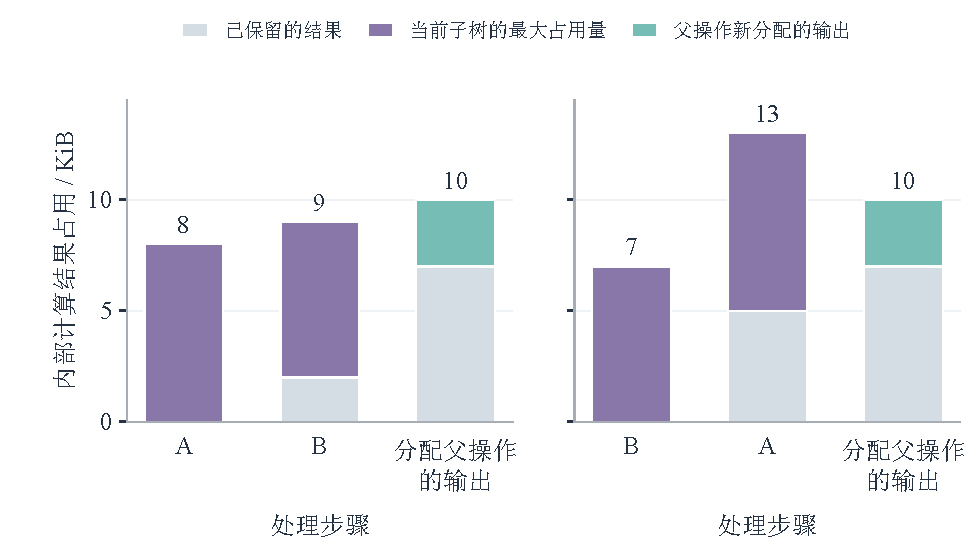
\includegraphics[width=\linewidth,height=.84\textheight,keepaspectratio]{figures/paper-v2/fig-forest-example.pdf}
\caption{两种子树处理顺序的内部结果占用。左：先A后B，峰值10 KiB；右：先B后A，峰值13 KiB。横轴为处理步骤，不是模拟时钟；数字为第6章的公式示例。}
\label{fig:forest-example}
\end{figure}

\subsection{非交错子树处理的最优顺序及证明}

设某个父算子拥有 \(m\) 棵待处理的子树，记 \(\pi = (\pi_1, \pi_2, \dots, \pi_m)\) 为这 \(m\) 棵子树的一个非交错处理排列次序，父算子自身输出张量大小记为 \(r_{\mathrm{parent}}\)。

在排列 \(\pi\) 下，当算法开始处理第 \(j\) 棵子树 \(\pi_j\) 时，前面已经处理完毕的 \(j - 1\) 棵子树所保留的根节点输出已累计占用 \(\sum_{\ell < j} r_{\pi_\ell}\) 字节，而处理当前子树 \(\pi_j\) 额外需要的最大内部临时存储为 \(h_{\pi_j}\) 字节；当全部 \(m\) 棵子树均处理完毕、父算子开始分配自身输出张量时，所有子树的输出尚未被释放，此时存储占用为 \(\sum_{i=1}^m r_i + r_{\mathrm{parent}}\) 字节。因此，排列 \(\pi\) 对应的全局存储峰值函数 \(H(\pi)\) 精确表示为：

\begin{equation}
H(\pi) = \max \left\{ \max_{1 \le j \le m} \left( \sum_{\ell < j} r_{\pi_\ell} + h_{\pi_j} \right), \ \sum_{i=1}^m r_i + r_{\mathrm{parent}} \right\}.
\end{equation}

该式中各项的物理单位均为字节（B）。

\textbf{命题6.1（子树存储最优排序）。} 若对所有子树均有 \(h_i \ge r_i \ge 0\)，则在上述非交错执行且父输出先分配的模型中，将子树按照指标差值 \(h_i - r_i\) 从大到小降序排列，能够使全局存储峰值 \(H(\pi)\) 取得最小值。

\begin{proof} 考虑排列中任意两个相邻的子树 A 与 B，设在当前序列中 A 紧邻且位于 B 之前。假设两者的指标满足 \(h_A - r_A \ge h_B - r_B\)。

在计算峰值时，暂时不考虑在处理 A 之前已经保留在存储中的其他前序子树输出常量 \(R_{\mathrm{prev}} = \sum_{\ell < \operatorname{pos}(A)} r_{\pi_\ell}\)。若按``先 A 后 B''的相对顺序执行，这两步操作期间局部达到的最大存储占用为：

\begin{equation}
H_{AB} = \max(h_A, \ r_A + h_B).
\end{equation}

若将 A 与 B 的执行顺序对调为``先 B 后 A''，对应的局部最大存储占用为：

\begin{equation}
H_{BA} = \max(h_B, \ r_B + h_A).
\end{equation}

由假设条件 \(h_A - r_A \ge h_B - r_B\) 移项可得：

\begin{equation}
r_A + h_B \le r_B + h_A.
\end{equation}

同时，由于物理保留量非负（\(r_B \ge 0\)）且子树内部峰值不小于保留量（\(h_A \ge r_A \ge 0\)），显然有：

\begin{equation}
h_A \le r_B + h_A.
\end{equation}

综合上述两式，可得：

\begin{equation}
H_{AB} = \max(h_A, \ r_A + h_B) \le r_B + h_A \le \max(h_B, \ r_B + h_A) = H_{BA}.
\end{equation}

前序已保留的常量 \(R_{\mathrm{prev}}\) 对两种次序的每一项产生完全相同的线性位移，不改变不等关系。并且，当 A 与 B 均处理完毕后，两者留在存储中的数据总和恒为 \(r_A + r_B\)，对后续其他子树的处理过程以及父算子输出 \(r_{\mathrm{parent}}\) 的分配不产生任何状态影响。

因此，若某个排列中存在相邻子树不满足 \(h_i - r_i\) 降序，将其交换位置绝不会导致全局存储峰值 \(H(\pi)\) 增大。通过有限次相邻逆序对的对调操作，任意排列均可转化为按 \(h_i - r_i\) 单调递减排列，且其峰值不增。自底向上递推应用于整棵树的各个归约节点，即证该贪心排列能够使模型内的存储峰值达到最优。 \end{proof}

该证明借鉴了经典树表达式代码生成与存储优化思想\cite{ref4}，并在本文所述的限定模型下给出了按字节度量存储占用的相邻交换证明。

需要强调的是，命题 6.1 证明的最优性受到严格的\textbf{模型适用边界}约束：

\begin{enumerate}
\def\labelenumi{\arabic{enumi}.}
\tightlist
\item
  结论仅适用于单棵孤立归约树、内部纯张量数据依赖、子树非交错处理的理想化模型；
\item
  该模型未考虑多核之间的并行交错、外部输入张量的重叠生命周期、L1 Buffer 与 UB 的独立物理容量分割；
\item
  该模型所得的标量存储峰值是用于指导排序的启发式代理（ordering proxy），它\textbf{并不等价于}官方底层编译流程中绝对不发生 Step 2 缓存换入换出（spill），亦\textbf{不直接等价于}离散事件仿真器推进下的多核 Makespan 最优。近期关于峰值内存调度的理论研究表明，面向一般有向无环图寻求支配调度或保持局部最优的拓扑线性化，需要特定的结构隔离条件\cite{ref10}；本文针对非交错归约树给出的 \(h_i - r_i\) 交换证明受限于单树模型，不外推为多流水线、动态 FIFO Cache 与完整 Makespan 的全局最优解。
\end{enumerate}

\subsection{森林调度实现的结构守卫与核心归属}

在算法实现中，为了将上述单树排序理论应用于输入计算图，程序构建了带有结构守卫的森林内存排序模块（\texttt{\seqsplit{forest\_memory\_order.py}}）。该模块并不假定所有输入图均能匹配树状模型，而是在进入优化前执行严密的结构验证。

\subsubsection{结构守卫与实现接受条件}

在本算法实现中，森林内存排序模块（\texttt{\seqsplit{forest\_memory\_order.py}}）针对输入计算图设定了明确的工程接受条件（guard conditions）。这些条件界定了当前代码所支持的结构范围，并非归约森林在数学图论上的充要定义：

\begin{enumerate}
\def\labelenumi{\arabic{enumi}.}
\tightlist
\item
  \textbf{多连通分量要求}：计算图在收缩边界 \texttt{COPY} 节点后的计算依赖图中，其无向连通分量数量必须至少为 2（\texttt{len(index.components)\ \textgreater{}=\ 2}）；
\item
  \textbf{各分量单一归约根}：每个连通分量内部必须构成一棵有向树，且每个分量包含且仅包含一个没有计算后继算子的根算子（root op）；
\item
  \textbf{汇合节点存在性}：整张计算图中必须至少存在一个拥有 2 个及以上前序输入算子的汇聚算子（join op，\texttt{joined\_nodes\ \textgreater{}=\ 1}）；
\item
  \textbf{计算出度无分叉}：除根节点外部输出外，所有计算算子的计算后继算子数量至多为 1（无 fanout，\texttt{outdegree\ \textless{}=\ 1}）；
\item
  \textbf{张量属性与唯一性}：计算图中所有张量具备已知的非负整数尺寸，且每个计算算子恰好生成一个内部输出张量；
\item
  \textbf{边界搬运严格规范}：计算图仅包含合法的边界 \texttt{COPY\_IN} 与 \texttt{COPY\_OUT} 算子，其中 \texttt{COPY\_IN} 必须将 DDR 外部输入映射为 L1 片上输入，\texttt{COPY\_OUT} 必须将根算子的 L1 输出写回 DDR，且输入输出张量大小完全一致；
\item
  \textbf{不支持直接算子依赖边}：若计算图中包含直接算子依赖边（direct op-op edges），由于无法确定对应的数据字节大小，模块将其视为超出当前排序实现范围的不支持结构，主动抛出异常（\texttt{\seqsplit{UnsupportedStructure}}）。
\end{enumerate}

上述结构守卫明确了本实现的工程支持边界；满足上述条件的输入图仍须经受实际评测的检验，算法不宣称满足这些条件即与全部底层硬件容量特征严密对应。

\subsubsection{核心归属与遍历次序生成}

在通过上述结构检验后，算法并不打破或重新搜索算子的计算核心分配，而是\textbf{严格保留由基准索引确定的核心归属映射（\texttt{\seqsplit{index.assignment(cores)}}）}。

算法以各连通分量为独立单元，自底向上递归计算各算子的 \((h_u, r_u)\) 属性，在每个汇聚节点处将前序子节点按 \(h_i - r_i\) 降序排序（相同指标下按算子 ID 破平）。随后，通过深度优先后序遍历（DFS postorder）为每个树分量生成算子执行序列。最后，在每个计算核心内部，将指派给该核心的各分量序列按照分量最小算子 ID 依次拼接，构造出满足单操作子图约束的候选调度方案。

\subsection{求解流水线与候选守卫机制}

在问题三的整体算法架构中，求解器继承并扩展了前序研发积累的流水线链条，形成了一条清晰的递进式父子演化链条：

\begin{equation}
\text{calendar\_solve} \longrightarrow \text{pipeline\_solve} \longrightarrow \text{witness\_solve} \longrightarrow \text{forest\_solve}.
\end{equation}

各层求解器通过分层守卫机制依次尝试不同的调度构型，并将全部尝试约束在统一的评测调用账本之下。

\subsubsection{递进式求解链条与候选生成}

\begin{enumerate}
\def\labelenumi{\arabic{enumi}.}
\tightlist
\item
  \textbf{\texttt{\seqsplit{calendar\_solve}}}：在问题二空闲区间调度的基础上，引入单核单操作子图的保底锚点（anchor），并针对大模型注意力计算（attention route）尝试构造基于 gap 的核心放置方案；
\item
  \textbf{\texttt{\seqsplit{pipeline\_solve}}}：调用 \texttt{\seqsplit{calendar\_solve}} 获得基准方案后，针对多核场景下的共享输入流水线结构，构造一种连续极小化极大划分（contiguous minimax partition）候选；
\item
  \textbf{\texttt{\seqsplit{witness\_solve}}}：调用 \texttt{\seqsplit{pipeline\_solve}} 获得前序最优方案后，若注意力计算路线在重新排序后评估代理变差，则生成一份保留原放置见证的候选方案（attention witness）；
\item
  \textbf{\texttt{\seqsplit{forest\_solve}}}：作为顶层求解模块，首先完整调用 \texttt{\seqsplit{witness\_solve}} 获取当前已知最优方案（incumbent winner）。若满足归约森林结构守卫，则生成基于本章树排序理论的 \texttt{\seqsplit{forest\_memory\_order}} 候选方案。
\end{enumerate}

\subsubsection{预算共用与终止状态分类}

整个求解流程在单次运行时\textbf{严格共用至多 3 次官方 E0 在线评测预算（\texttt{\seqsplit{total\_e0\_limit\ =\ 3}}）}。在 \texttt{\seqsplit{forest\_solve}} 阶段，系统对候选方案的状态转移实施精细化管理：

\begin{enumerate}
\def\labelenumi{\arabic{enumi}.}
\tightlist
\item
  \textbf{预算耗尽跳过（\texttt{\seqsplit{skip:\ three\_call\_budget\_already\_used}}）}：若前序父求解器（如 calendar、pipeline、witness）已累计发起了 3 次评测请求，则当前阶段不再生成亦不再评测 forest 候选方案，直接输出当前最优方案；
\item
  \textbf{结构不支持跳过（\texttt{\seqsplit{skip:\ UnsupportedStructure}}）}：若输入计算图不满足归约森林的结构守卫，模块安全捕获异常并跳过，保持当前方案输出；
\item
  \textbf{方案完全重复（\texttt{duplicate}）}：若生成的 \texttt{\seqsplit{forest\_memory\_order}} 方案与当前最优方案的代码表示完全一致，则记录为重复状态，不发起重复评测；
\item
  \textbf{完成时间下界剪枝（\texttt{\seqsplit{bound\_pruned}}）}：对生成的候选方案求解其不可避免的物理完成时间下界 \(L\)。若 \(L \ge U\)（\(U\) 为当前已知最优方案的官方 Makespan），则该候选在数学上绝无可能超越当前最优解，算法直接放弃评测；
\item
  \textbf{下界不支持但允许评测（\texttt{\seqsplit{UnsupportedBound}}）}：若候选方案超出下界分析模块支持的范畴，系统仅记录 \texttt{\seqsplit{bound\_unavailable}}，\textbf{绝不直接拒绝候选方案}，依然允许其进入后续评测流程；
\item
  \textbf{严格选优准则}：仅当候选方案通过官方评测且其最终 Makespan 严格小于当前最优解（\(M < U\)）时，方接受该方案并替换为新的最优解。\textbf{在问题三的决策逻辑中，不使用 DDR 搬运量进行平局决选（tie-break）}。
\end{enumerate}

\subsection{固定候选方案的完成时间下界}

为了在发起昂贵的官方评测之前安全剔除无希望的候选方案，算法设计了针对静态调度方案的完成时间下界分析器（\texttt{\seqsplit{pipe\_bound.py}}）。

\subsubsection{下界模型的构造、守卫条件与数学形式}

该分析器（\texttt{\seqsplit{pipe\_bound.py}}）针对已完全排定次序的静态调度方案生效，其适用范围受如下守卫条件（guards）严格约束：

\begin{enumerate}
\def\labelenumi{\arabic{enumi}.}
\tightlist
\item
  \textbf{算子与流水线范围}：每个子图必须恰好包含一个原始非 COPY 算子，且所有计算算子的流水线类型仅限 \texttt{PIPE\_M} 与 \texttt{PIPE\_V}；
\item
  \textbf{计算周期非负整数}：算子计算时长满足 \(d_u = \max(1, \text{cycles}_u)\)，其中原始 \(\text{cycles}_u\) 必须为非负整数；
\item
  \textbf{依赖提取与保守拒绝}：依赖关系仅由计算图的原始张量流动与直接算子边提取；若排除边界 COPY 收缩后引入了无法证明的附加依赖（\texttt{ambiguous} 依赖），或加入同核流水线次序弧后增广图出现环路，分析器均主动抛出 \texttt{\seqsplit{UnsupportedBound}} 异常退出；
\item
  \textbf{合法性范围声明}：该模块仅证明在给定次序下成功物理执行的完成时间下界，\textbf{并不构成}该调度方案满足官方全部编译依赖或硬件执行合法性的证明。
\end{enumerate}

当方案通过上述守卫后，方案在任何一次成功的物理执行中，各算子的启动时刻必定受到一组必要时序不等式的严格约束：

\begin{enumerate}
\def\labelenumi{\arabic{enumi}.}
\tightlist
\item
  \textbf{数据依赖不等式}：若算子 \(u\) 与算子 \(v\) 存在直接张量依赖或直接算子依赖，则 \(v\) 的启动时刻满足： \begin{equation}
s_v \ge s_u + d_u + \delta_{uv}.
\end{equation} 其中，若 \(u\) 与 \(v\) 被分配到不同的计算核心，计入跨核心通信引发的硬件延迟 \(\delta_{uv} = 500\text{ cycles}\)（该数值对应冻结的 P3 官方配置）；若在同一核心，则 \(\delta_{uv} = 0\)。同一对算子间若存在多个并列依赖约束，系统取延迟的最大值（\(\max\)），不进行代数累加；
\item
  \textbf{同核同流水线 FIFO 约束}：在同一计算核心内部，分配给同一类执行流水线（如 \texttt{PIPE\_M}）的各个算子必须按照调度方案排定的先后次序单串行推进执行。若在该核心的该流水线上算子 \(u\) 紧排在算子 \(v\) 之前，则必有： \begin{equation}
s_v \ge s_u + d_u.
\end{equation}
\end{enumerate}

依据上述必要不等式，记 \(ES(v)\) 为算子 \(v\) 的最早可能启动时刻。对于无前序约束的初始就绪算子，令其候选基准为 0；对于一般算子 \(v\)，其最早启动时刻严格满足拓扑动态规划式：

\begin{equation}
ES(v) = \max \left( \{0\} \cup \left\{ ES(u) + d_u + \delta_{uv} \ \middle|\ (u, v) \in \mathcal{E}_{\mathrm{bound}} \right\} \right).
\end{equation}

整份方案的物理完成时间下界 \(L(P)\) 定义为所有算子执行完成时刻的最大值（空图时取 0）：

\begin{equation}
L(P) = \begin{cases} \displaystyle \max_{v \in V} \bigl( ES(v) + d_v \bigr), & V \ne \emptyset, \\ 0, & V = \emptyset. \end{cases}
\end{equation}

该下界完全由底层硬件执行的必要不等式推导得出。若当前系统已经取得了一份完成时间为 \(U\) 的合法方案，且计算得出 \(L(P) \ge U\)，则该候选方案在实际执行中的 Makespan 必然满足 \(M \ge L(P) \ge U\)，绝不可能严格优于现有结果，从而可以被安全剪除。需要指出的是，该下界是必要约束界定的理论底线，并不宣称其数值必然等于消除外部瓶颈后实际可达的调度耗时；相较之下，任意放松约束后运行贪心启发式算法所得的耗时仅代表某一种可行排程的完成时间，并不构成理论下界。

\subsection{算法步骤与复杂度分析}

\textbf{算法3：问题三多核心协同调度算法（P3 Forest Solver）。}

\begin{lstlisting}[style=gmcmappendix,language={}]
输入：原始计算图 G、计算核心数 K、官方硬件配置 config。
输出：合法的切分与调度方案 P = (node_to_subgraph, core_schedules)。
1. 初始化官方评测调用计数 calls = 0，评测上限 limit = 3；
2. 调用前序父求解器 witness_solve，在其内部依次尝试 calendar、pipeline 与 witness 策略：
     若产生合法方案且评测 Makespan 改善，更新当前最优解 winner 与当前耗时上界 U；
3. 检查评测账本：若 calls >= limit，直接返回当前 winner；
4. 检查计算图 G 是否满足归约森林结构守卫（连通分量 >= 2、无出度分叉、每算子单一确定尺寸输出、无直接计算依赖边等）：
     若不满足，安全捕获 UnsupportedStructure 异常，跳过后续构造，直接返回 winner；
5. 保持基准分量核心分配不变，提取各分量算子树，自底向上计算各节点 (h_u, r_u) 指标；
6. 汇聚节点处按 (h_i - r_i) 降序排定子树顺序，通过 DFS 后序遍历生成各分量执行序列；
7. 拼接生成候选调度方案 proposal，检查其唯一性：
     若 proposal 与 winner 方案完全一致，标记为 duplicate 并返回 winner；
8. 尝试构建 proposal 的依赖与流水线 FIFO 必要约束图，计算有向图最长路径下界 L(proposal)：
     若成功求得下界且 L(proposal) >= U：
         标记为 bound_pruned，省去评测，直接返回 winner；
     若抛出 UnsupportedBound 异常：
         记录 bound_unavailable，继续推进后续流程；
9. 发起官方离散事件仿真评测（calls = calls + 1）：
     若评测异常或未通过合法性检查，记录 rejected 并返回 winner；
     若评测成功且 Makespan < U：
         更新 winner = proposal，更新 U = Makespan；
10. 返回最终胜出的最佳方案 winner。
\end{lstlisting}

\subsubsection{算法时间复杂度解耦分析}

算法在求解过程中的计算耗时由以下几个相互独立的计算环节组成：

\begin{enumerate}
\def\labelenumi{\arabic{enumi}.}
\tightlist
\item
  \textbf{森林识别与拓扑分析}：在无向连通分量与依赖拓扑提取中，对计算算子及连通分量的遍历耗时为 \(O(V + E)\)；
\item
  \textbf{自底向上指标递推与子树排序}：自叶向根递推计算各节点存储指标需 \(O(V)\) 时间。在每个汇聚节点处对其子节点进行排序，设节点 \(v\) 的入度（即前序子树数量）为 \(\deg(v)\)，全图排序的总时间复杂度为： \begin{equation}
O\left( \sum_{v \in V} \deg(v) \log \deg(v) \right) \le O(V \log V).
\end{equation}
\item
  \textbf{深度优先后序遍历与方案拼接}：生成各分量 DFS 序列与拼接核心序列耗时为 \(O(V)\)；
\item
  \textbf{必要时序图最长路径求解}：若候选方案满足单操作 M/V 算子条件，构建包含 \(V\) 个节点与 \(E_{\mathrm{bound}}\) 条约束弧的有向无环图，利用拓扑排序计算最长路径的时间复杂度为 \(O(V + E_{\mathrm{bound}})\)；
\item
  \textbf{官方离散事件仿真评测开销}：在全流程至多 \(b \le 3\) 次在线评测调用中，仿真耗时表示为 \(\sum_{j=1}^b T_j\)，其中 \(T_j\) 取决于官方离散事件仿真器的内部模拟事件量。
\end{enumerate}

需要明确说明的是，上述森林排序部分的复杂度界仅适用于该排序生成逻辑本身，并不包含外部全局 \texttt{Index} 索引构建、初始分量核心指派（\texttt{assignment}）以及官方底层编译与仿真评测的全局耗时，避免将整个求解流程错误归属为线性或低多项式复杂度。同时，评测次数上限为常数（\(\le 3\)）亦不构成全流程计算时间的代数证明，求解耗时的可控性根本上依赖于前置结构守卫与下界剪枝的配合。

\subsection{启用和关闭共享缓存的配对实验}

本文算法（Forest 固定版本，源码对应 Commit \texttt{311322b}）在官方提供的 100 张全量基准计算图、涵盖 1 至 5 核心的全部 500 种测试组合上进行了完整的端到端求解与评测，所有方案均顺利通过官方合法性校验。测试结果依据 \texttt{\seqsplit{paper/manuscript-v1/data/all-results.csv}} 与固定数据资产进行了严格复核。

在全量 500 个测试组合的求解过程中，求解器累计发起 973 次在线 E0 评测，未触发任何重试。与前一完整策略相比，全网格共有 24 个用例实现了 Makespan 的进一步缩短，其余 476 个用例持平，零退化（degrade = 0）。在额外数据搬运量（\texttt{\seqsplit{extra\_ddr\_bytes}}）与由于片上容量不足引发的搬运量（\texttt{\seqsplit{spill\_bytes}}）方面，各有 18 个用例显著减少，479 个用例持平，3 个用例增加，两项统计指标均实现了 \(413{,}450{,}240\) 字节的净减少。

为深入量化共享只读 Cache 对系统性能的实际影响，实验对同一套生成的 P3 最终方案分别在``关闭 Cache（无 L2）''与``开启 Cache''两种官方评测配置下进行了成对（paired）仿真对比。下表汇总了各核心数下的测试数据（注意：表中``无 L2''列代表同一份 P3 方案在关闭 Cache 时的表现，并非由问题二算法独立生成的方案）：

{\def\LTcaptype{table} % do not increment counter
\begin{table}[!htbp]\centering\small
\begin{tabular}{@{}
  >{\raggedright\arraybackslash}p{(\linewidth - 8\tabcolsep) * \real{0.1579}}
  >{\raggedleft\arraybackslash}p{(\linewidth - 8\tabcolsep) * \real{0.2105}}
  >{\raggedleft\arraybackslash}p{(\linewidth - 8\tabcolsep) * \real{0.2105}}
  >{\raggedleft\arraybackslash}p{(\linewidth - 8\tabcolsep) * \real{0.2105}}
  >{\raggedleft\arraybackslash}p{(\linewidth - 8\tabcolsep) * \real{0.2105}}@{}}
\toprule\noalign{}
\begin{minipage}[b]{\linewidth}\raggedright
计算核心数量
\end{minipage} & \begin{minipage}[b]{\linewidth}\raggedleft
无 L2：\(\operatorname{mean}(B/M_2)\)
\end{minipage} & \begin{minipage}[b]{\linewidth}\raggedleft
开启 Cache：\(\operatorname{mean}(B/M_3)\)
\end{minipage} & \begin{minipage}[b]{\linewidth}\raggedleft
成对加速比均值 \(\operatorname{mean}(M_2/M_3)\)
\end{minipage} & \begin{minipage}[b]{\linewidth}\raggedleft
逐用例字节命中率算术平均
\end{minipage} \\
\midrule\noalign{}


1 & 1.1971 & 1.1998 & 1.0023 & 6.47\% \\
2 & 2.2949 & 2.3120 & 1.0079 & 16.25\% \\
3 & 3.1745 & 3.2587 & 1.0314 & 25.96\% \\
4 & 3.9211 & 4.0915 & 1.0512 & 24.53\% \\
5 & 4.4763 & 4.7576 & 1.0829 & 31.36\% \\
\bottomrule\end{tabular}
\end{table}
}

表中数据展现了如下规律：

\begin{enumerate}
\def\labelenumi{\arabic{enumi}.}
\tightlist
\item
  \textbf{Cache 带来的增益表现}：在 1 至 5 核心下，开启 Cache 后方案的平均加速比从无 Cache 时的 1.1971、2.2949、3.1745、3.9211 与 4.4763，分别提升至 1.1998、2.3120、3.2587、4.0915 以及 4.7576。逐用例成对加速比均值 \(\operatorname{mean}(M_2/M_3)\) 在 5 核心场景下达到 1.0829；
\item
  \textbf{指标口径的精确区分}：表中第一、二列的分母基准 \(B\) 均严格采用官方单核基准方案的 Makespan。第三列为逐用例计算 \(M_2/M_3\) 后的算术平均值（\(1.0829\)），该数值在数学上并不等于两列均值的直接相除（\(\frac{4.7576}{4.4763} \approx 1.0628\)）；
\item
  \textbf{缓存命中率的统计差异}：在 5 核心场景下，逐用例字节命中率的算术平均值为 31.36\%。若将全量 100 张图的全部访问请求汇总后统一计算，按整体访问字节加权的总字节命中率为 47.45\%。两者差异源于不同计算图的通信规模不均，访问数据量庞大的计算图在加权统计中占据了更高比重；
\item
  \textbf{求解端到端耗时分布}：包含在线评测在内，求解程序在 500 个用例上的物理墙钟时间均值为 4.401 秒，中位数为 1.616 秒，95\% 分位数（最近秩次法，第 475 位）为 20.009 秒，最大值为 51.335 秒。
\end{enumerate}

\begin{figure}[!htbp]
\centering
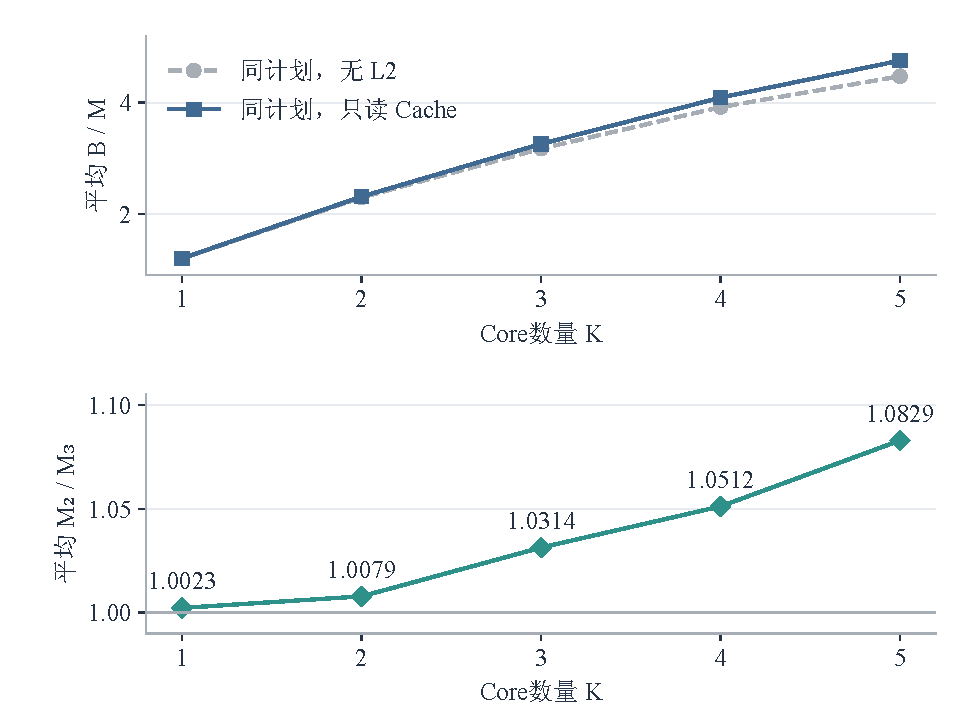
\includegraphics[width=\linewidth,height=.84\textheight,keepaspectratio]{figures/paper-v2/fig-p3-results.pdf}
\caption{问题三的保持方案不变的配对评价。上：无 L2 与只读 Cache 的平均基线加速比；下：逐图$M_2/M_3$的均值，每种核心数量包含100对结果。}
\label{fig:p3-results}
\end{figure}

\begin{figure}[!htbp]
\centering
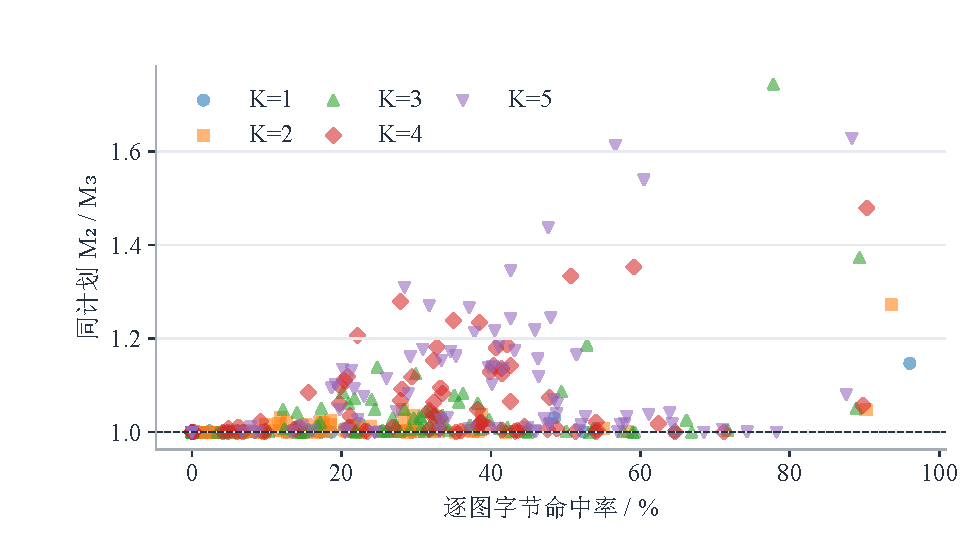
\includegraphics[width=\linewidth,height=.84\textheight,keepaspectratio]{figures/paper-v2/fig-cache-gain.pdf}
\caption{500 个保持方案不变的配对结果中的字节命中率与 Cache 收益。保留低于 1 的负收益点；100 个用例的不同核心数量结果相关，不能当作 500 个独立随机样本。}
\label{fig:cache-gain}
\end{figure}

\subsection{附加比值选择条件的反例与消融（R9F）}

为了探索能否通过在在线评测阶段增加多重评价指标以进一步优化 Cache 利用效果，前期研发中曾设计了一组附加筛选条件的对照实验（代码代号为 R9F）。

在 R9F 策略中，设计者对 5 核心的候选方案设置了三项必须同时满足的严格筛选准则：

\begin{enumerate}
\def\labelenumi{\arabic{enumi}.}
\tightlist
\item
  开启 Cache 后的完成时间严格缩短（\(M_{3, \mathrm{new}} < M_{3, \mathrm{old}}\)）；
\item
  关闭 Cache 后的完成时间不退化（\(M_{2, \mathrm{new}} \le M_{2, \mathrm{old}}\)）；
\item
  Cache 带来的相对改善比值不下降，即 \(G_{\mathrm{new}} \ge G_{\mathrm{old}}\)，其中比值定义为 \(G = \frac{M_2}{M_3}\)。
\end{enumerate}

在 5 核心的 100 张基准计算图中，96 张图由于不符合该策略的特定前置结构而跳过，1 张图被下界分析模块提前剪枝，其余 3 张图生成了候选方案并进入了在线评测。然而，这 3 张图生成的候选方案均因未能同时满足上述三项准则而被判定拒绝，最终 R9F 输出的 500 份方案与 Forest 主算法完全一致。

对这 3 张被拒绝用例的深层数据复核揭示了一个关键反例现象：这三份被拒绝的候选方案在实际执行中，\textbf{其实同时显著缩短了 \(M_2\) 与 \(M_3\)}，具体数值如下表所示：

{\def\LTcaptype{table} % do not increment counter
\begin{table}[!htbp]\centering\small
\begin{tabular}{@{}
  >{\raggedright\arraybackslash}p{(\linewidth - 8\tabcolsep) * \real{0.1579}}
  >{\raggedleft\arraybackslash}p{(\linewidth - 8\tabcolsep) * \real{0.2105}}
  >{\raggedleft\arraybackslash}p{(\linewidth - 8\tabcolsep) * \real{0.2105}}
  >{\raggedleft\arraybackslash}p{(\linewidth - 8\tabcolsep) * \real{0.2105}}
  >{\raggedleft\arraybackslash}p{(\linewidth - 8\tabcolsep) * \real{0.2105}}@{}}
\toprule\noalign{}
\begin{minipage}[b]{\linewidth}\raggedright
测试用例 / 核心数
\end{minipage} & \begin{minipage}[b]{\linewidth}\raggedleft
原方案 \(M_2\) / cycles
\end{minipage} & \begin{minipage}[b]{\linewidth}\raggedleft
候选方案 \(M_2\) / cycles
\end{minipage} & \begin{minipage}[b]{\linewidth}\raggedleft
原方案 \(M_3\) / cycles
\end{minipage} & \begin{minipage}[b]{\linewidth}\raggedleft
候选方案 \(M_3\) / cycles
\end{minipage} \\
\midrule\noalign{}


case\_064 / 5 Core & 7,029 & 6,899 & 6,981 & 6,877 \\
case\_068 / 5 Core & 131,631 & 98,913 & 116,345 & 97,971 \\
case\_088 / 5 Core & 97,305 & 66,729 & 85,789 & 66,224 \\
\bottomrule\end{tabular}
\end{table}
}

因为执行完成时间恒为正整数，准则 3 中要求的比值不下降条件可严格展开为代数乘积形式：

\begin{equation}
G_{\mathrm{new}} \ge G_{\mathrm{old}} \iff \frac{M_{2, \mathrm{new}}}{M_{3, \mathrm{new}}} \ge \frac{M_{2, \mathrm{old}}}{M_{3, \mathrm{old}}} \iff M_{2, \mathrm{new}} \cdot M_{3, \mathrm{old}} \ge M_{2, \mathrm{old}} \cdot M_{3, \mathrm{new}}.
\end{equation}

以 \texttt{case\_088} 为例，原方案的指标为 \(M_2 = 97{,}305\) cycles，\(M_3 = 85{,}789\) cycles，比值 \(G_{\mathrm{old}} \approx 1.1342\)。候选方案将无 Cache 时的完成时间大幅压缩至 \(M_{2, \mathrm{new}} = 66{,}729\) cycles（缩短了 31.42\%），同时将开启 Cache 时的完成时间压缩至 \(M_{3, \mathrm{new}} = 66{,}224\) cycles（缩短了 22.81\%）。由于无 Cache 场景下的优化幅度超越了有 Cache 场景下的优化幅度，导致新方案的比值下降为 \(G_{\mathrm{new}} \approx 1.0076 < G_{\mathrm{old}}\)。该比值准则因此直接判定该候选不合格并予以抛弃。

这一消融实验清楚地证明：在多目标多场景评估中，人为构造的复合比值指标容易产生与核心目标背离的掩盖效应，反而排除了在官方模拟中能够大幅缩短执行时间的优秀方案。本文主算法 Forest 坚持以官方规定的主口径 Makespan 严格单调下降作为唯一的接受准则，确保了优化方向始终紧密对准赛题的首要目标。


\section{实验结果与分析}

\subsection{评测基准、对比设定与统计口径}

本文算法在官方赛题指定的全部 100 张原始计算图上展开系统性实验，计算核心数量依次配置为 1 至 5 核心，每道题目涵盖 500 种``计算图---核心数''测试组合，三道题目合计完成 1500 组完整的端到端求解与仿真评测。针对每一道题目，实验均采用运行前已完全冻结的单一固定求解器程序版本，其内部策略选择规则、候选生成数量以及在线评测调用上限在运行前全部固化，不针对特定算题进行人工微调。

实验数据由统一的数据资产库（\texttt{\seqsplit{paper/manuscript-v1/data/all-results.csv}} 与 \texttt{\seqsplit{source-receipt.json}}）导出并复核。全文分析依托于三类明确的对比维度：

\begin{enumerate}
\def\labelenumi{\arabic{enumi}.}
\tightlist
\item
  \textbf{相对官方单核心基准的加速比}：以官方提供的单核心基准方案完成时间除以算法输出方案的完成时间，严格计算每一测试用例的加速比，并计算算术平均值；
\item
  \textbf{算法版本演进的宏观对比}：比较同一计算图和同一核心数下，不同完整算法版本之间的整体性能演进。由于每个主版本通常包含结构识别、核心放置与顺序调整等多项改进，宏观版本对比用于展示系统综合能力的提升，不将整体增益简单归因于单一机制的孤立贡献；
\item
  \textbf{共享只读 Cache 的成对隔离对比}：针对问题三生成的同一份最终调度方案，保持任务切分与排程完全不变，分别在关闭 Cache（无 L2）与开启 Cache 两种官方硬件配置下运行离散事件仿真，严格度量共享 Cache 对同一物理调度方案执行时钟周期的纯收益。
\end{enumerate}

\begin{figure}[!htbp]
\centering
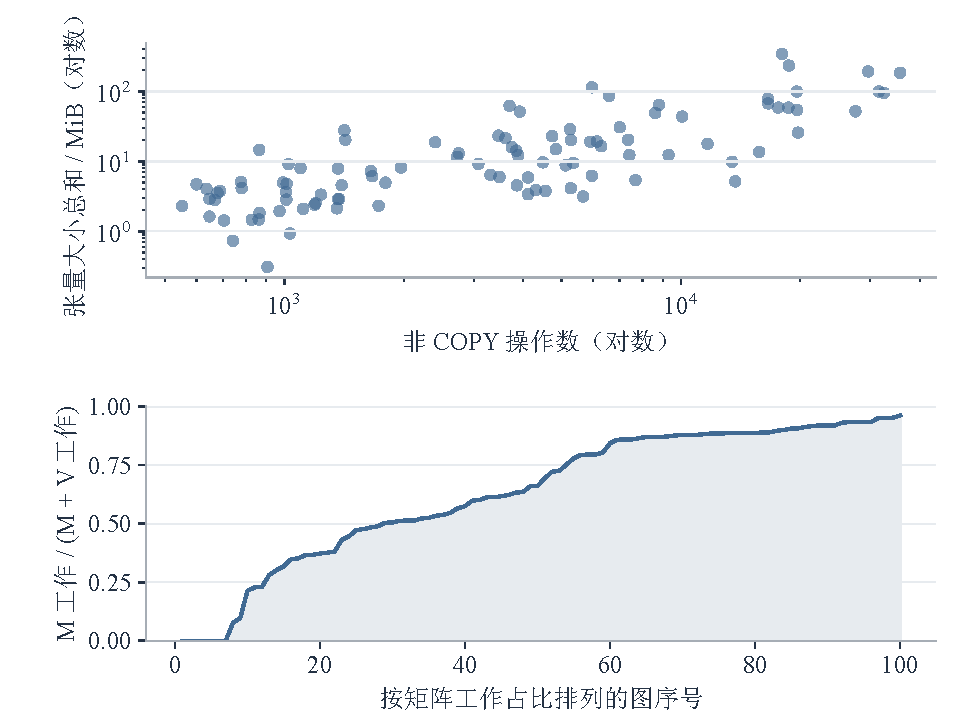
\includegraphics[width=\linewidth,height=.84\textheight,keepaspectratio]{figures/paper-v2/fig-dataset.pdf}
\caption{官方 100 张计算图的结构统计。上：非 COPY 操作数与张量大小总和；下：按矩阵计算的时长占两类计算总时长的比例排序的用例分布。}
\label{fig:dataset}
\end{figure}

\subsection{三问主口径加速比综合对比}

下表汇总了问题一（P1）、问题二（P2）与问题三（P3）的主算法输出方案，在 1 至 5 核心下的平均加速比。表中每格数值均基于该核心数下的 100 张基准计算图逐用例计算 \(B/M\) 后取算术平均，三道题目统一采用官方提供的单核心基准完成时间 \(B\) 作为基准分子：

{\def\LTcaptype{table} % do not increment counter
\begin{table}[!htbp]\centering\small
\begin{tabular}{@{}
  >{\raggedright\arraybackslash}p{(\linewidth - 8\tabcolsep) * \real{0.1579}}
  >{\raggedleft\arraybackslash}p{(\linewidth - 8\tabcolsep) * \real{0.2105}}
  >{\raggedleft\arraybackslash}p{(\linewidth - 8\tabcolsep) * \real{0.2105}}
  >{\raggedleft\arraybackslash}p{(\linewidth - 8\tabcolsep) * \real{0.2105}}
  >{\raggedleft\arraybackslash}p{(\linewidth - 8\tabcolsep) * \real{0.2105}}@{}}
\toprule\noalign{}
\begin{minipage}[b]{\linewidth}\raggedright
计算核心数量
\end{minipage} & \begin{minipage}[b]{\linewidth}\raggedleft
P1 优化方案
\end{minipage} & \begin{minipage}[b]{\linewidth}\raggedleft
P2 优化方案
\end{minipage} & \begin{minipage}[b]{\linewidth}\raggedleft
P3 优化方案（开启 Cache）
\end{minipage} & \begin{minipage}[b]{\linewidth}\raggedleft
P3 同方案（无 L2 运行）
\end{minipage} \\
\midrule\noalign{}


1 & 1.0021 & 1.2061 & 1.1998 & 1.1971 \\
2 & 1.9516 & 2.3167 & 2.3120 & 2.2949 \\
3 & 2.7514 & 3.2356 & 3.2587 & 3.1745 \\
4 & 3.4786 & 3.9711 & 4.0915 & 3.9211 \\
5 & 4.0553 & 4.5498 & 4.7576 & 4.4763 \\
\bottomrule\end{tabular}
\end{table}
}

三道题目之间的性能演进直接反映了硬件执行语义与调度算法的协同深化：

\begin{enumerate}
\def\labelenumi{\arabic{enumi}.}
\tightlist
\item
  \textbf{硬件执行语义的演进}：

  \begin{itemize}
  \tightlist
  \item
    问题一要求各个硬件执行任务（Task）之间传递的数据必须经由外部主存（DDR）中转，跨 Task 数据搬运产生显著的 DDR 访存开销，同时同核相邻任务切换伴随 100 cycles 上下文开销、跨核依赖伴随 1000 cycles 同步等待；
  \item
    问题二与问题三引入同核心任务合并机制，被分配到同一核心的算子可直接在片上私有缓存（L1 Buffer 与 UB）中复用数据，彻底消除了核内核间不必要的数据往返；
  \item
    问题三进一步引入 1 MiB 的共享只读 Cache，为多核心共享的静态张量提供了高速片上访问链路，进一步降低了 DDR 带宽负载；
  \end{itemize}
\item
  \textbf{指标统计口径的严谨区分}：

  \begin{itemize}
  \tightlist
  \item
    表中第 4 列``P3 优化方案''与第 5 列``P3 同方案无 L2''由同一份 P3 调度方案在不同硬件仿真模式下评测得出；而第 3 列``P2 优化方案''是由问题二专用求解器独立优化生成的不同调度方案；
  \item
    在 5 核心场景下，P3 方案在开启 Cache 与关闭 Cache 时的平均加速比分别为 4.7576 与 4.4763，两列平均值直接相除的比值为 \(\frac{4.7576}{4.4763} \approx 1.0628\)；而依据第 2 章定义，逐用例计算两者的成对加速比 \(M_2/M_3\) 后的算术平均值为 \(1.0829\)。产生差异的原因在于各用例的完成时间基数分布不均，本文以逐用例成对计算的算术平均值作为衡量 Cache 收益的主口径；
  \item
    在单核心场景下，P2 与 P3 算法输出方案的 Makespan 相比官方单核基准分别取得了 1.2061 与 1.1998 的 \(B/M\) 比值，表明算法重排算子次序后在单核上亦能提升指令流水线的重叠密度。
  \end{itemize}
\end{enumerate}

\subsection{求解效率与在线评测调用统计}

算法的端到端求解耗时包含原始计算图解析、拓扑分析与候选构造、必要下界计算、在线代理与官方评测推进，以及最终合法方案的磁盘写入。

为了客观呈现求解效率，下表将三道题目的统计范围统一为全量 500 种测试组合（涵盖 100 张图、1 至 5 核心）。95\% 分位数（P95）统一严格采用最近秩次法（nearest-rank，取排序后第 \(\lceil 0.95n \rceil\) 个观测值，样本量 \(n=500\) 时对应第 475 位）：

{\def\LTcaptype{table} % do not increment counter
\begin{table}[!htbp]\centering\small
\begin{tabular}{@{}
  >{\raggedright\arraybackslash}p{(\linewidth - 10\tabcolsep) * \real{0.1364}}
  >{\raggedleft\arraybackslash}p{(\linewidth - 10\tabcolsep) * \real{0.1818}}
  >{\raggedleft\arraybackslash}p{(\linewidth - 10\tabcolsep) * \real{0.1818}}
  >{\raggedleft\arraybackslash}p{(\linewidth - 10\tabcolsep) * \real{0.1818}}
  >{\raggedleft\arraybackslash}p{(\linewidth - 10\tabcolsep) * \real{0.1818}}
  >{\raggedright\arraybackslash}p{(\linewidth - 10\tabcolsep) * \real{0.1364}}@{}}
\toprule\noalign{}
\begin{minipage}[b]{\linewidth}\raggedright
求解器与题目范围
\end{minipage} & \begin{minipage}[b]{\linewidth}\raggedleft
在线评测总调用账本
\end{minipage} & \begin{minipage}[b]{\linewidth}\raggedleft
求解耗时均值 / s
\end{minipage} & \begin{minipage}[b]{\linewidth}\raggedleft
P95 耗时 / s
\end{minipage} & \begin{minipage}[b]{\linewidth}\raggedleft
最大耗时 / s
\end{minipage} & \begin{minipage}[b]{\linewidth}\raggedright
运行主机与并发环境
\end{minipage} \\
\midrule\noalign{}


P1 求解器（全量 500 组合） & 1130 次 E1 评测（48 次 E0 复核 + 452 次核同复用） & 2.825 & 13.164 & 25.552 & 共享多核主机，4 个并发进程 \\
P2 求解器（全量 500 组合） & 1131 次原生 E2 评测（0 次 E0 回退） & 4.029 & 18.841 & 40.187 & 共享多核主机，1 个独占进程 \\
P3 Forest（全量 500 组合） & 973 次原生 E0 评测（0 次异常重试） & 4.401 & 20.009 & 51.335 & 共享多核主机，4 个并发进程 \\
\bottomrule\end{tabular}
\end{table}
}

针对问题一在 5 核心场景（100 个样本，对应第 95 位）下的独立统计，其求解耗时均值为 3.522 秒，P95 为 16.623 秒，最大耗时为 25.552 秒。

如表中数据所示：

\begin{enumerate}
\def\labelenumi{\arabic{enumi}.}
\tightlist
\item
  \textbf{调用预算与守卫有效性}：在三道题目各自 500 次独立求解过程中，在线评测调用次数平均每用例仅发起约 2 次（均严格控制在设定的上限以内），说明自适应选择、拓扑守卫与前置下界剪枝机制有效规避了无希望候选的盲目评测；
\item
  \textbf{端到端求解时间}：在所有 1500 次运行中，最长单例求解耗时为 51.335 秒，全部用例的物理耗时均远远低于赛题建议的 5～10 分钟时间范围。由于测试运行于共享主机且并发进程数不同，各题间的耗时差异反映工程运行实际记录，不作为独占硬件条件下的算力性能排序。
\end{enumerate}

\begin{figure}[!htbp]
\centering
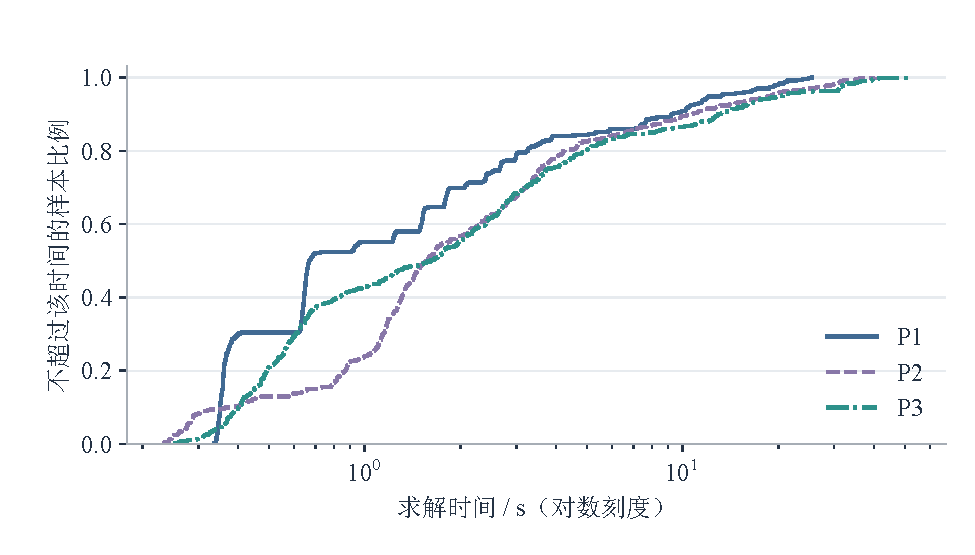
\includegraphics[width=\linewidth,height=.84\textheight,keepaspectratio]{figures/paper-v2/fig-runtime.pdf}
\caption{三种求解程序的实际经过时间累计分布，每题500次。时间包含方案构造及在线评价，横轴采用对数刻度；批次资源不同，不据此比较独占机器的速度。}
\label{fig:runtime}
\end{figure}

\subsection{算法消融分析与反例证据}

为了检验各项机制的实际影响并验证设计假设，实验针对关键组件与对照策略进行了消融对比与反例检验。在多处理器系统性能分析中，单纯统计局部算子耗时并不直接对应全局完成时间的因果改善\cite{ref12}；若多个机制同时演变，不能将整版本的宏观收益直接归因于单一孤立机制：

\begin{enumerate}
\def\labelenumi{\arabic{enumi}.}
\tightlist
\item
  \textbf{问题一分支援助与重排策略}：在问题一中，引入分支重排与前沿细化后，5 核心场景下的平均加速比提升约 0.729\%，全图额外 DDR 搬运总量微增约 0.389\%。这表明算法通过局部容忍合理的边界搬运，换取了计算算子在多核心流水线上的并发展开；
\item
  \textbf{问题二超图连接度模型与工作量守卫}：与前一完整版本相比，P2 求解器在全量 500 个测试组合中有 268 个用例缩短了 Makespan，232 个用例持平，零退化。与此同时，500 个用例的额外 DDR 搬运总量增加了 36.66\%。深入的用例分析显示，Makespan 缩短与搬运量增加高度共存，印证了以执行时间为首要目标的权衡准则是有效的；
\item
  \textbf{C04 对照策略的限定反例}：针对前期实验策略 C04 的 6 个 5 核心用例对比显示，C04 方案虽然经官方 Step 2 编译确认未发生任何片上缓存换入换出（spill 为 0），且跨核心边界搬运字节数显著低于主算法，但其最终 Makespan 全面劣化（在 \texttt{case\_019} 上变慢 75.50\%）。这一反例表明单纯优化静态搬运量并不能保证执行时间缩短；
\item
  \textbf{问题三树状内存排序的收益}：P3 Forest 求解器在全量 500 个测试组合中，使 24 个用例的 Makespan 进一步获得显著缩短，476 个用例持平；全网格额外 DDR 搬运量与溢出搬运量各净减少 \(413{,}450{,}240\) 字节（18 个用例减少，479 个持平，3 个增加）；
\item
  \textbf{R9F 复合比值准则的消融反例}：在 5 核心下对候选方案附加 \(G_{\mathrm{new}} \ge G_{\mathrm{old}}\)（即 \(M_2/M_3\) 不下降）等三重准则的 R9F 对照实验中，有 3 个候选用例（\texttt{case\_064}、\texttt{case\_068}、\texttt{case\_088}）虽然在实际执行中同时显著缩短了无 Cache 耗时 \(M_2\) 与开启 Cache 耗时 \(M_3\)，但因无 Cache 耗时的压缩幅度更大导致比值数值下降，从而被复合准则错误拒绝。该消融实验表明，在多场景多目标评估中，人为构造的复合比值指标可能对主优化目标产生负面干扰。
\end{enumerate}

\subsection{完成时间理论下界与最优性差距}

为了评估算法输出方案与理论极限的接近程度，实验利用静态调度下界分析器对问题二各核心数下的方案质量进行了数学上界检验。

对于任意输入计算图，设 \(L\) 为在给定单操作子图和流水线次序下、由硬件依赖与 FIFO 不等式证明的物理完成时间下界，设当前算法求得的实际方案完成时间为 \(U\)。由于任意合法执行的物理完成时间 \(\mathrm{OPT}\) 必然满足 \(L \le \mathrm{OPT} \le U\)，因此相对偏差比值 \(\frac{U}{L} - 1\) 给出了算法当前方案与理论最优解之间相对误差的\textbf{保守数学上限}。

依据固定的 P2 理论下界评测记录：

\begin{enumerate}
\def\labelenumi{\arabic{enumi}.}
\tightlist
\item
  \textbf{高精度达标分布}：在 1 至 5 核心下，分别有 81、62、32、33 与 23 张基准计算图严格满足 \(U \le 1.05 L\)。即在当前声明的硬件条件下，这些测试用例输出方案的 Makespan 与理论物理极限的偏差不超过 5\%；
\item
  \textbf{多核松弛间隙演变}：在 5 核心场景下，全量计算图的平均下界加速比 \(\operatorname{mean}(B/L)\) 约为 6.108，高于算法实际达到的平均加速比 4.550。这一差距反映出静态下界模型松弛了片上存储容量竞争、总线读写仲裁以及跨核心复杂通信等动态瓶颈，因此 6.108 是理论松弛边界，并非在真实物理硬件上已证实可达的加速比。
\end{enumerate}

\begin{figure}[!htbp]
\centering
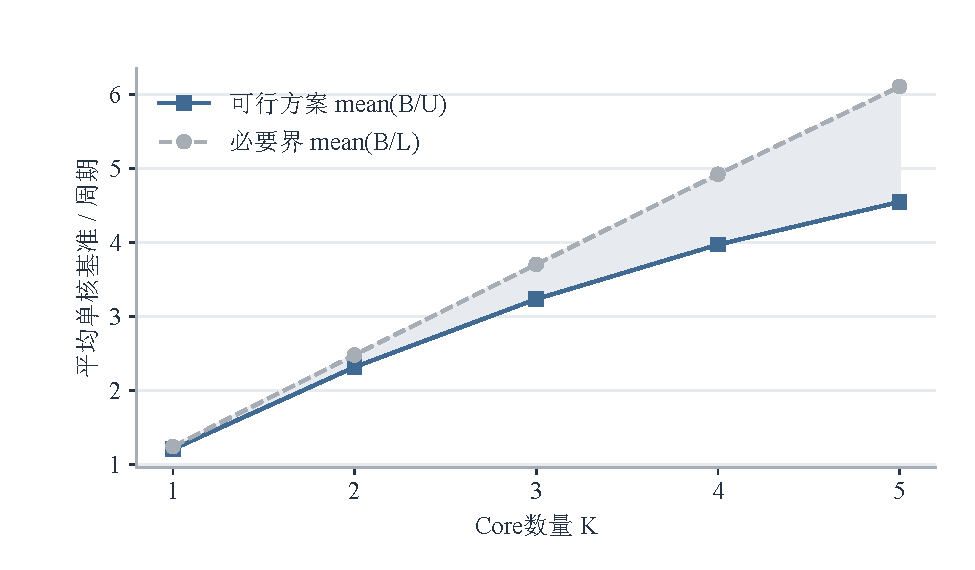
\includegraphics[width=\linewidth,height=.84\textheight,keepaspectratio]{figures/paper-v2/fig-bound-gap.pdf}
\caption{同一输入、配置与方案范围下的时间上界和下界。$L\le\mathrm{OPT}\le U$，阴影是必要界给出的上限与当前结果之间的差距，不代表一定可实现的收益。}
\label{fig:bound-gap}
\end{figure}

\subsection{实验范围与评估局限}

本文实验结果受如下客观条件与研究范围的制约：

\begin{enumerate}
\def\labelenumi{\arabic{enumi}.}
\tightlist
\item
  \textbf{样本关联性与统计范围}：测试所用的全部 100 张官方计算图在前期研发中均作为基准参与过特征分析。由于同一张计算图在 1 至 5 核心下的拓扑结构完全一致，不同核心数下的测试结果存在高度的内在关联性，不可将其视为 500 个独立同分布的统计样本进行假设检验；
\item
  \textbf{结构自适应与通用性}：算法内部的分支选择依据图的无向连通分量数量、算子出度以及流水线工作量等拓扑结构特征自动决策，避免了按用例编号显式查表，但其在完全未见的外部工业模型计算图上的表现仍有待进一步实测验证；
\item
  \textbf{仿真环境与真机执行差异}：方案的最终质量指标（Makespan 与额外搬运量）完全由官方离散事件仿真器（\texttt{\seqsplit{schedule\_step2.py}} 与 \texttt{\seqsplit{schedule\_step3.py}}）推进计算得出，求解耗时由本机物理墙钟秒数记录。仿真模型高度还原了硬件周期与仲裁机制，但本研究尚未在真实的神经网络处理器（NPU）芯片上部署驱动并开展真机板级测量。
\end{enumerate}


\section{方法评价与结论}

\subsection{主要方法与适用范围}

本文共同确定算子划分、核心分配与执行顺序三个决策维度：

\begin{enumerate}
\def\labelenumi{\arabic{enumi}.}
\tightlist
\item
  \textbf{问题一}：识别无依赖的计算分支并在核心间重新分配，均衡各核心计算流水线的工作量，结合前沿细化权衡并行收益与搬运开销；
\item
  \textbf{问题二}：构建超图连接度模型刻画多算子张量复用，推导预 Step 2 原始复制字节数，并在二核心局部调整中通过流水线工作量上限保护机制防止计算向单核过度倾斜；
\item
  \textbf{问题三}：针对满足接受条件的归约森林结构，依据各子树内部峰值与保留输出的差值降序排定非交错执行顺序，并在候选方案上构建必要时序图最长路径下界以过滤低效搜索。
\end{enumerate}

各章节的数学分析针对明确的物理与图论问题提供依据：通过标号偏序证明扩展依赖图不存在死锁环路；通过超边连接度模型解释同时移动多个消费算子与边界复制量的阶跃关系；通过相邻子树对调证明在非交错执行模型下使内部结果存储峰值最小的排序准则；通过底层必要不等式建立完成时间下界以快速剪除缺乏潜力的候选方案。这些理论性质均受限于所设定的结构模型，不替代底层的离散事件评测。

算法在实际应用中受以下条件制约：

\begin{enumerate}
\def\labelenumi{\arabic{enumi}.}
\tightlist
\item
  \textbf{动态硬件争用与模型松弛}：总线带宽争用、Cache 动态插入逐出以及片上存储空间分配存在复杂的时序交织。理论文献中针对有界树宽图在允许资源松弛的条件下建立了双指标完全多项式时间近似方案（FPTAS）\cite{ref11}；然而本题涉及张量动态生命周期、硬性片上容量约束以及共享只读 Cache 的 FIFO 逐出，无法直接继承该类近似保证；
\item
  \textbf{结构假设与适用范围}：森林内存排序与下界分析依赖于特定的图结构特征。若算子存在跨分支的多重消费（fanout），或包含未指定张量大小的直接计算边，则无法直接套用该排序模型；
\item
  \textbf{评价准则的设计权衡}：如 C04 与 R9F 消融实验所示，单纯优化静态通信量或人为引入复合比值门槛可能导致放弃完成时间更短的方案，决策逻辑仍须紧密围绕主口径 Makespan 展开。
\end{enumerate}

\subsection{结论}

本文实现的三个固定求解器版本，在官方指定的全部 100 张基准计算图、涵盖 1 至 5 核心的 1500 种测试组合上完成了全部评测。在 5 核心配置下，问题一、二、三的平均基线加速比分别达到 4.0553、4.5498 与 4.7576；在保持问题三方案不变的前提下，开启共享只读 Cache 相比关闭 Cache 的逐用例平均加速比为 1.0829。

方案完成时间由官方评测程序推进的离散事件仿真时钟周期（cycles）度量，求解效率由物理机执行墙钟秒数度量；本文所呈现的数据反映在规定基准与配置下的模拟测试记录，不代表在真实 NPU 芯片上的板级实测结果。实验表明，通过图拓扑与硬件特征构造少量结构化方案，结合理论必要条件实施护栏剪枝，并利用受限的在线评测预算进行综合决选，能够在赛题建议的高效时间范围内稳定获得符合官方目标的调度解。


\FloatBarrier
\begin{thebibliography}{12}
\bibitem{ref1} 第二十三届中国研究生数学建模竞赛. A题：通用神经网络处理器下的多核调度问题及官方附件{[}Z{]}. 2026.
\bibitem{ref6} POPP M, SCHLAG S, SCHULZ C, SEEMAIER D. Multilevel Acyclic Hypergraph Partitioning{[}C{]}//2021 Proceedings of the Symposium on Algorithm Engineering and Experiments (ALENEX). 2021: 1--15. DOI: 10.1137/1.9781611976472.1.
\bibitem{ref7} ÖZKAYA M Y, ÇATALYÜREK Ü V. A Simple and Elegant Mathematical Formulation for the Acyclic DAG Partitioning Problem{[}EB/OL{]}. arXiv:2207.13638, 2022. {[}2026-09-26{]}. https://arxiv.org/abs/2207.13638. DOI: 10.48550/arXiv.2207.13638.
\bibitem{ref2} GRAHAM R L. Bounds for Certain Multiprocessing Anomalies{[}J{]}. Bell System Technical Journal, 1966, 45(9): 1563--1581. DOI: 10.1002/j.1538-7305.1966.tb01709.x.
\bibitem{ref5} BLACK P E. Hyperedge; Hypergraph{[}EB/OL{]}. Dictionary of Algorithms and Data Structures, NIST. {[}2026-09-26{]}. https://xlinux.nist.gov/dads/HTML/hyperedge.html.
\bibitem{ref3} ÇATALYÜREK Ü V, AYKANAT C. Hypergraph-Partitioning-Based Decomposition for Parallel Sparse-Matrix Vector Multiplication{[}J{]}. IEEE Transactions on Parallel and Distributed Systems, 1999, 10(7): 673--693. DOI: 10.1109/71.780863.
\bibitem{ref8} VELDT N, BENSON A R, KLEINBERG J. Hypergraph Cuts with General Splitting Functions{[}J{]}. SIAM Review, 2022, 64(3): 650--685. DOI: 10.1137/20M1321048.
\bibitem{ref9} DINIC E A. An algorithm for the solution of the max-flow problem with the polynomial estimation{[}J{]}. Soviet Mathematics Doklady, 1970, 11: 1277--1280.
\bibitem{ref4} SETHI R, ULLMAN J D. The Generation of Optimal Code for Arithmetic Expressions{[}J{]}. Journal of the ACM, 1970, 17(4): 715--728. DOI: 10.1145/321607.321620.
\bibitem{ref10} JIN C, PUROHIT M, SVITKINA Z, VEE E, WANG J R. New Tools for Peak Memory Scheduling{[}EB/OL{]}. arXiv:2312.13526, 2023. {[}2026-09-26{]}. https://arxiv.org/abs/2312.13526. DOI: 10.48550/arXiv.2312.13526.
\bibitem{ref12} CURTSINGER C, BERGER E D. Coz: Finding Code that Counts with Causal Profiling{[}C{]}//Proceedings of the 25th Symposium on Operating Systems Principles. 2015: 184--197. DOI: 10.1145/2815400.2815409.
\bibitem{ref11} ANGEL E, MORAIS S, REGNAULT D. A Bi-Criteria FPTAS for Scheduling with Memory Constraints on Graphs with Bounded Tree-Width{[}C{]}//Euro-Par 2022: Parallel Processing. LNCS 13440. 2022: 136--151. DOI: 10.1007/978-3-031-12597-3\_9.
\end{thebibliography}

\appendix
\section{逐用例结果与单位}

\texttt{\seqsplit{data/all-results.csv}} 保存三题共 1500 种图与核心数量组合的完整测试结果。每行记录包含题号、图编号、计算核心数、单核心基线 Makespan、多核 Makespan、额外 DDR 搬运字节数、端到端求解耗时及结果来源哈希；问题三另行记录关闭 L2 时的对照结果与 Cache 字节命中率。

由于全量 1500 行数据表格篇幅较大，完整数据清单独立排版于附录文档 \texttt{\seqsplit{result-tables.pdf}} 中供查阅，正文实验章节保留核心统计指标、均值、分位数与标准物理单位。数据表格中，执行时间以周期（cycle）为单位，数据量以字节（B）为单位，命中率以百分比呈现。正文所有聚合统计均基于未舍入的原始数据进行精确计算。数据来源文件及其 SHA-256 校验和在 \texttt{\seqsplit{data/source-receipt.json}} 中逐项注册，以确保实验记录的一致性与可溯源性。

\section{补充数学推导}

\subsection{数据依赖所给出的完成时间下界}

本节假设每个需要讨论的原图中间张量至多由一个原始计算操作生成，不同原始张量标识不合并成同一逻辑数据标识。取出原始计算操作，只保留有依据的先后关系，包括原来就存在的计算关系，以及同一张量的生成操作必须先于读取操作的关系。不任意缩短经过原始 COPY 的路径。

在任何官方成功执行中，这些计算操作及其时长都被保留，每个核心的每条 Pipe 也仍同时至多处理一个操作。直接取该次执行中各计算的核心和开始、完成时刻，就得到满足保留关系的一组安排。因此，在这些必要关系下求得的最小必要时间，不会大于官方完成时间。

对于分配到不同核心的计算操作，必须核对两者之间的依赖怎样在官方执行中保留。问题一要求相关前驱 Task 完成后，后续 Task 才允许开始；问题二、三要求源 COPY\_OUT 完成，再经过 500 cycles，目标 COPY\_IN 才可参与就绪判断；实际开始仍需满足其余数据依赖、执行单元和存储条件。接收端若因容量不足而需要再次读入数据，还受官方 Step 2 次序和 MTE2 操作队列顺序限制，不能跳过所需的基础 COPY\_IN。上述必要关系均从官方成功执行所满足的条件中提取。

\subsection{指定时间区间内的工作量下界}

在 B.1 的计算操作之间的数据依赖图上，为操作 \(v\) 定义两个不包括自身的时长：\(h_v\) 为它之前最长依赖路径的时长，\(t_v\) 为它之后最长依赖路径的时长。无相应前驱或后继时取 0。递推式为：

\begin{equation}
h_v = \max_{u \to v}(h_u + d_u), \qquad t_v = \max_{v \to w}(d_w + t_w).
\end{equation}

本节 \(h_v\) 以 cycle 计，与第 6 章按字节定义的子树存储量 \(h_i\) 是不同的局部记号。取 \(a, b \ge 0\)，选定一种 Pipe \(p\)，考虑非空操作集合：

\begin{equation}
S = \{v: p_v = p, \ h_v \ge a, \ t_v \ge b\}.
\end{equation}

任何成功执行中，\(S\) 的操作都只能完整安排在 \([a, M - b]\) 内：它们之前至少需要 \(a\) 个周期，之后至少需要 \(b\) 个周期。同类 Pipe 共有 \(K\) 个，每个操作又不能拆成多段交给不同核心。因此，除了总工作量，还可以利用操作不可分割这一条件。

将 \(S\) 中 \(n\) 个操作的时长降序排列为 \(d_{(1)} \ge \cdots \ge d_{(n)}\)。定义：

\begin{equation}
A_K(S) = \max_{\substack{r \ge 1 \\ m = (r-1)K+1 \le n}} \sum_{j=m-r+1}^{m} d_{(j)}.
\end{equation}

于是：

\begin{equation}
M \ge a + b + \max\left\{\left\lceil\frac{\sum_{v \in S} d_v}{K}\right\rceil, A_K(S)\right\}.
\end{equation}

\begin{proof} 令 \(x = M - a - b\)，\(K\) 个同类 Pipe 在该区间内最多提供 \(Kx\) 个计算周期，得到第一项。取前 \(m = (r-1)K + 1\) 个操作，至少一个核心要执行其中 \(r\) 个；即使选其中最短的 \(r\) 个，也至少需要 \(\sum_{j=m-r+1}^{m} d_{(j)}\) 周期。对允许的 \(r\) 取最大得到第二项。两项都限制同一个区间的长度，故取最大值，不相加。最后只加一次前后所需的 \(a + b\)。 \end{proof}

例如，两个核心执行三个不可拆分操作，时长分别为 10、8、7 cycles。总工作量给出 13 cycles 的下界，上式利用不可分割性给出 15 cycles。达到 15 仍可能受其他依赖和资源限制，这个例子只说明下界为何能加强。

图上递推 \(h_v, t_v\) 需要 \(O(n + m)\) 时间；固定 \(a, b\) 后，检查集合成员需 \(O(n)\)，对选中操作排序需 \(O(|S| \log |S|)\)。枚举所有 \(a, b\) 还要另计成本。若 \(S\) 为空，不能仅凭 \(a + b\) 得到有效下界。

\subsection{计算工作量与不同核心之间的等待约束}

考虑一串按数据依赖拓扑排序、先后存在确定依赖关系的特定计算算子序列 \(u_0 \to u_1 \to \cdots \to u_m\)，将其作为相邻时间区间的边界分隔操作。为保证后文各区间的完成时间下界能够直接线性相加，所选区间必须严格互不重叠且在拓扑上具有确定的前后依赖链关系。任取若干缺乏全局全序关系的汇合节点并不足以支撑区间的可加性。

对于由相邻分隔算子 \(u_{i-1}\) 与 \(u_i\) 划定的局部时间区间，考察落在该区间内部且绑定在同一种执行流水线（Pipe）\(p\) 上的非空计算操作子集 \(S \subseteq V_{\mathrm{comp}} \setminus \{u_{i-1}, u_i\}\)（不含分隔操作自身）。对每个操作 \(v \in S\)，严格定义其局部的内部前后依赖耗时：

\begin{itemize}
\tightlist
\item
  前端内部计算耗时 \(h_i(v)\)：以左边界分隔操作 \(u_{i-1}\) 完成时刻为时间零点，定义为从 \(u_{i-1}\) 到 \(v\) 的内部前驱计算操作路径时长（仅累加内部前驱计算算子的固有执行时长，不含 \(u_{i-1}\) 与 \(v\) 自身；若为无中间计算操作的直接依赖则取 0；若存在多条路径则取该 \(v\) 对应的最长路径）；
\item
  后端内部计算耗时 \(t_i(v)\)：定义为从 \(v\) 完成到右边界分隔操作 \(u_i\) 开始时刻所需的内部后继计算路径时长（仅累加内部后继计算算子的固有执行时长，不含 \(v\) 与 \(u_i\) 自身；若为直接依赖则取 0；若存在多条路径则取该 \(v\) 对应的最长路径）。
\end{itemize}

不能将附录 B.2 中相对于全图源汇点全局定义的 \(h_v, t_v\) 直接代入局部区间。选取统一阈值对 \(a, b \ge 0\) 时，必须取非负整数周期（\(a, b \in \mathbb{N}\)）以保证后续有效窗口 \(z = x - a - b\) 为确定离散整数周期，且必须满足集合 \(S\) 内的所有操作 \(v \in S\) 均有 \(h_i(v) \ge a\) 且 \(t_i(v) \ge b\)（等价于 \(a \le \min_{v \in S} h_i(v)\) 且 \(b \le \min_{v \in S} t_i(v)\)）；亦可先选定非负整数阈值 \(a, b \ge 0\)，再据此筛选满足条件的非空同流水线集合 \(S = \{v \in V_{\mathrm{comp}} \setminus \{u_{i-1}, u_i\} : \operatorname{pipe}(v) = p, h_i(v) \ge a, t_i(v) \ge b\}\)。严禁将 \(a, b\) 定义为整个集合 \(S\) 的最长依赖路径。集合 \(S\) 中的每个受约束操作，必须存在经附录 B.1 官方硬件语义验证的边界依赖路径。若考察的区间处于计算图最前端（无前驱分隔操作），则令 \(\ell = 0\) 且 \(a = 0\)；若处于计算图最末端（无后继分隔操作），则令 \(r = 0\) 且 \(b = 0\)；当区间两端均存在确定分隔操作时，令 \(\ell = 1, r = 1\)。

对于被分配至不同核心的计算操作，跨核心硬件依赖等待常数记为 \(\tau_q\)（依据附录 B.1 经官方验证的硬件语义：问题一跨 Task 硬件同步屏障为 \(\tau_1 = 1000\) cycles；问题二与问题三跨核心搬运等待下界为 \(\tau_2 = \tau_3 = 500\) cycles；该等待下界仅在硬件规则明确支持的范围内生效）。为精确区分操作分配核心与边界核心的关系，定义逐操作的核心归属指示变量：若左边界分隔操作 \(u_{i-1}\) 存在（\(\ell = 1\)）且操作 \(v\) 所在核心与左边界核心不同（即 \(\operatorname{core}(v) \ne \operatorname{core}(u_{i-1})\)），则令 \(\delta_L(v) = 1\)，否则令 \(\delta_L(v) = 0\)；类似地，若右边界分隔操作 \(u_i\) 存在（\(r = 1\)）且 \(\operatorname{core}(v) \ne \operatorname{core}(u_i)\)，则令 \(\delta_R(v) = 1\)，否则令 \(\delta_R(v) = 0\)。结合内部依赖阈值与跨核等待，当存在对应侧分隔操作时，任意 \(v \in S\) 的开始执行时刻与完成时刻满足： \begin{equation}
\operatorname{start}(v) \ge \text{left\_end} + \max(a, \delta_L(v) \tau_q), \qquad \operatorname{finish}(v) \le \text{right\_start} - \max(b, \delta_R(v) \tau_q),
\end{equation} 其中 \(\text{left\_end}\) 为左边界完成时刻，\(\text{right\_start}\) 为右边界开始时刻（若某一侧不存在分隔操作，则直接使用计算图整体执行的起止边界）。

指标 \(\ell, r \in \{0, 1\}\) 仍用于表征边界存在性及定义跨核心残余等待。扣除区间内部计算已覆盖的重叠时间后，同时不同于两个存在边界核心的其他核心所受的残余纯等待时间下界为：

\begin{equation}
c(a,b) = \ell(\tau_q - a)_+ + r(\tau_q - b)_+,
\end{equation}

其中 \((x)_+ = \max(x, 0)\)。当两端边界指派在同一核心时，该核心自身完全不受这两个跨核等待约束，拥有完整的有效计算窗口 \(z\)；当两端边界位于不同核心时，各边界所在核心分别只受另一端的跨核约束，而其余 \(K - 2\) 个既不承担左边界也不承担右边界的核心则同时承受两端的残余等待限制。

设该局部时间区间的物理跨度为整数周期 \(x \ge a + b\)，扣除前后内部计算耗时后，可供集合 \(S\) 中操作并发执行的有效时间窗口为整数周期 \(z = x - a - b \ge 0\)。对应流水线上的总计算工作量为 \(W(S) = \sum_{v \in S} d_v\)。若前后两个分隔操作指派在同一核心，该核心在窗口内最多可提供 \(z\) 个周期，其他核心受跨核传输等待约束，各至多提供 \((z - c)_+\) 个有效计算周期，故有：

\begin{equation}
W(S) \le z + (K - 1)(z - c)_+.
\end{equation}

若前后分隔操作位于不同核心（此时必有 \(K \ge 2\)），令 \(A = (\tau_q - a)_+\)，\(B = (\tau_q - b)_+\)。各核心可供同类流水线使用的总周期数至多为：

\begin{equation}
(z - A)_+ + (z - B)_+ + (K - 2)(z - A - B)_+.
\end{equation}

由于实数运算中恒有 \((z - A)_+ + (z - B)_+ \le z + (z - A - B)_+\)，上述单核心主导不等式对跨核心情形同样构成有效上界约束。对于离散整数周期，满足工作量约束所需的最小有效窗口时长为：

\begin{equation}
\phi_{K,c}(W) = \min\left\{W, \left\lceil\frac{W + (K - 1)c}{K}\right\rceil\right\}.
\end{equation}

结合单个算子在物理流水线上不可跨核心拆分的离散限制，该局部区间的最小物理耗时下界为：

\begin{equation}
x \ge a + b + \max\{\phi_{K, c(a,b)}(W(S)), A_K(S)\}.
\end{equation}

仅当各个区间之间严格互不重叠且由拓扑依赖链串联时，各区间的下界与分隔算子自身的执行周期方可直接线性求和累加（分隔算子自身执行时长另行计入）。若仅考察局部相互重叠的滑动窗口，则只能取各窗口下界的最大值，绝不可重复累加。此外，问题一中同一核心内部不同 Task 切换所引入的 100 cycles 切换开销，由于具体方案未必在所选算子边界处切分子图，不能作为必要下界无条件计入。若上述任一前提条件无法满足，则该下界公式仅在其实际成立的受限子图范围内生效，不予强行推广。

由上述推导可见，与前后计算重叠的等待时间已被严格扣除，各时间段仅计算一次。本节为离线补充理论推导，正文下界统计使用的是第 7 章所列已有版本的结果。

\subsection{状态信息充分性的判定条件}

本节讨论一个尚未由本文主算法一般实现的理论问题：能否仅保存方案的部分抽象状态信息，即可完全无损地判定后续结构修改的可行性及其执行结果。两份方案当前离散模拟的 Makespan 相同，并不足以说明它们在未来的修改演化中等价。例如，两份方案可能具有不同的核心内子图执行拓扑次序，某项算子迁移修改在第一份方案中合法可行，而在第二份方案中却可能诱发循环依赖死锁。

为了形式化分析状态信息的充分性，必须同时固定输入计算图 \(G\)、计算核心总数 \(K\)、赛题问题编号 \(q\) 以及官方硬件配置（\texttt{config}），并固定官方评测源码版本（Commit SHA）、底层解释器与执行环境，以及完整的确定性实现约定（包括稳定的算子排序、字典迭代顺序、平局决胜规则以及浮点精度）。需要明确的是，源码提交哈希本身并不单独保证跨平台环境下的位级一致性，确定性行为的严格成立依赖于执行环境与实现约定的共同固定。设 \(\mathcal{P}\) 为声明的合法调度方案域，定义一组允许对方案施加的确定性原子修改动作集合 \(\mathcal{A}\)（例如在声明的结构范围内移动、合并或拆分子图；每项动作的参数含义与执行逻辑严格确定）。对于任意动作 \(a \in \mathcal{A}\)，记能够合法执行该动作的方案子集为 \(D_a \subseteq \mathcal{P}\)。我们假设动作转移具有确定性，且声明的方案域 \(\mathcal{P}\) 对允许动作封闭，即：

\begin{equation}
\forall a \in \mathcal{A}, \forall P \in D_a \implies a(P) \in \mathcal{P}.
\end{equation}

设 \(\Phi(P)\) 为从方案 \(P\) 中提取的观测结果。若仅考察正常完成的执行，可取观测结果为 Makespan；若涵盖可能出现的执行异常，则须将成功或失败的离散状态编码入观测向量中，而不能为未定义的执行赋予臆想的周期数值。

令 \(\mathcal{L}(P)\) 为从方案 \(P\) 出发、能够依次连续施加的所有有限动作序列集合（包含不施加任何修改的空序列 \(\epsilon\)）。两份方案 \(P\) 与 \(Q\) 在动作系统 \(\mathcal{A}\) 下等价，要求它们诱导的可执行动作序列集合完全相同，且在任意相同动作序列作用后的观测结果完全一致：

\begin{equation}
\mathcal{L}(P) = \mathcal{L}(Q), \qquad \Phi(w(P)) = \Phi(w(Q)), \quad \forall w \in \mathcal{L}(P),
\end{equation}

其中 \(w(P)\) 表示按序列 \(w\) 中的动作顺次对方案 \(P\) 实施转移。

\textbf{命题B.1（状态充分性条件）。} 在同时固定输入计算图 \(G\)、计算核心数 \(K\)、问题场景 \(q\)、官方硬件配置参数、评测源码版本、参考执行环境以及确定性约定的条件下，假设动作转移具有确定性且方案域 \(\mathcal{P}\) 对 \(\mathcal{A}\) 封闭。设 \(S: \mathcal{P} \to \mathcal{X}\) 为对方案提取的抽象状态函数。若针对每一个原子动作 \(a \in \mathcal{A}\)，均存在前置可行性判定函数 \(d_a: \mathcal{X} \to \{\text{True}, \text{False}\}\)、状态更新函数 \(\bar{a}: \mathcal{X} \to \mathcal{X}\) 以及全局观测恢复函数 \(o: \mathcal{X} \to \mathcal{Y}\)，使得对于方案域内的任意方案 \(P \in \mathcal{P}\) 均满足：

\begin{equation}
P \in D_a \iff d_a(S(P)), \qquad S(a(P)) = \bar{a}(S(P)) \quad (\forall P \in D_a), \qquad \Phi(P) = o(S(P)),
\end{equation}

则 \(S(P) = S(Q)\) 必能充分推导出方案 \(P\) 与 \(Q\) 的行为等价性（即 \(\mathcal{L}(P) = \mathcal{L}(Q)\) 且 \(\Phi(w(P)) = \Phi(w(Q))\) 对任意 \(w \in \mathcal{L}(P)\) 恒成立）。

\begin{proof} 当动作序列为空序列 \(\epsilon\) 时，由 \(S(P) = S(Q)\) 及观测恢复条件直接得到 \(\Phi(P) = o(S(P)) = o(S(Q)) = \Phi(Q)\)。假设对于任意长度不超过 \(k\) 的可执行动作序列 \(w = (a_1, a_2, \dots, a_k)\)，均有 \(w \in \mathcal{L}(P) \iff w \in \mathcal{L}(Q)\)，且转移后方案仍满足 \(S(w(P)) = S(w(Q))\)。对于任意追加动作 \(a_{k+1} \in \mathcal{A}\)，由于可行性判定函数 \(d_{a_{k+1}}\) 仅依赖于状态 \(S\)，由 \(S(w(P)) = S(w(Q))\) 可知： \begin{equation}
w(P) \in D_{a_{k+1}} \iff d_{a_{k+1}}(S(w(P))) \iff d_{a_{k+1}}(S(w(Q))) \iff w(Q) \in D_{a_{k+1}}.
\end{equation} 因此长度为 \(k+1\) 的序列在两方案上同时可行或同时不可行。若该动作可行，由于方案域封闭性，转移后方案依然落在 \(\mathcal{P}\) 内，由状态更新等式可得： \begin{equation}
S(a_{k+1}(w(P))) = \bar{a}_{k+1}(S(w(P))) = \bar{a}_{k+1}(S(w(Q))) = S(a_{k+1}(w(Q))).
\end{equation} 进而通过观测恢复函数导出两者的观测完全一致：\(o(S(a_{k+1}(w(P)))) = o(S(a_{k+1}(w(Q)))) = \Phi(a_{k+1}(w(P))) = \Phi(a_{k+1}(w(Q)))\)。由数学归纳法可知，等价性结论对任意有限长度的可执行动作序列均严格成立。 \end{proof}

需要明确的是，命题 B.1 仅给出了状态信息足以支撑无损预测的充分条件，并未证明该状态表示在信息论或状态复杂度意义下达到了最小表示（极小商空间），亦未假定微架构全局响应具有简单的可加性。若要证明状态的最小性，必须进一步证明任意两个不同的抽象状态均存在某条测试动作序列能够将其观测区分开。本文求解器在实现上并未构建此类通用行为商空间，而是针对具体的搜索算子实施轻量级局部校验与字节级哈希去重；本节推导系基于本文模型独立核验的条件性理论界限，旨在为未来探索状态折叠与受控搜索空间压缩提供严谨的判定基准。

\section{固定实现与复现入口}

{\def\LTcaptype{table} % do not increment counter
\begin{table}[H]\centering\small
\begin{tabular}{@{}
  >{\raggedright\arraybackslash}p{(\linewidth - 6\tabcolsep) * \real{0.2500}}
  >{\raggedright\arraybackslash}p{(\linewidth - 6\tabcolsep) * \real{0.2500}}
  >{\raggedright\arraybackslash}p{(\linewidth - 6\tabcolsep) * \real{0.2500}}
  >{\raggedright\arraybackslash}p{(\linewidth - 6\tabcolsep) * \real{0.2500}}@{}}
\toprule\noalign{}
\begin{minipage}[b]{\linewidth}\raggedright
问题
\end{minipage} & \begin{minipage}[b]{\linewidth}\raggedright
固定源码提交
\end{minipage} & \begin{minipage}[b]{\linewidth}\raggedright
模块入口
\end{minipage} & \begin{minipage}[b]{\linewidth}\raggedright
在线评价次数上限
\end{minipage} \\
\midrule\noalign{}


P1 & \texttt{\seqsplit{834d8c957538ee069c66aadac9509552a4cc69d7}} & \texttt{\seqsplit{src.q1.branch\_refine}} & 10次E1 \\
P2 & \texttt{\seqsplit{c66559a6f8a31ef7b4720e1f7c3c28d61f8dff3f}} & \texttt{\seqsplit{src.q2\_nikolastarx.adaptive\_hypergap\_guarded}} & 3次E2 \\
P3 & \texttt{\seqsplit{311322b996c0948e8a6a9c7ec6ddfe6ae41fbee1}} & \texttt{\seqsplit{src.q3.forest\_solve}} & 3次E0 \\
\bottomrule\end{tabular}
\end{table}
}

表中固定提交（P1 为 \texttt{\seqsplit{834d8c957538ee069c66aadac9509552a4cc69d7}}，P2 为 \texttt{\seqsplit{c66559a6f8a31ef7b4720e1f7c3c28d61f8dff3f}}，P3 为 \texttt{\seqsplit{311322b996c0948e8a6a9c7ec6ddfe6ae41fbee1}}）及其完整依赖共同确定各算法的复现版本。附录 E 所导出的 7 个核心算法模块为展示核心逻辑的独立源码切片，其运行时依赖项仍须溯源至上述固定提交，并非脱离代码仓即可独立运行的自包含脚本。官方代码哈希为 \texttt{\seqsplit{de11a83db8d7c47ed328b15a7df71d613a833b16cd23ee9fe877999578a1ace0}}，配置哈希为 \texttt{\seqsplit{dcd10de54b23f8366428fb24e828812b1da9549e6eae4a3c3f38604fe5ae77b9}}。

已有结果可在保留相关 Git 对象的仓库中，通过运行 \texttt{\seqsplit{python3\ paper/manuscript-v1/scripts/export\_tables.py}} 重新导出。该命令仅读取冻结数据，不调用求解器或评价器。

\section{图中各类数据的含义}

原图片段保留节点编号、张量字节数和裁剪外的依赖。真实执行时间线绑定相同输入、方案、核心数量和官方配置，各区间来自官方事件；数学示例明确注明是示例，不使用未经模拟的执行时刻。

两种方案的 Task 和 Pipe 时间线共用坐标尺度。空白区间只表示没有操作执行，只有事件记录能够支持时才说明原因。Cache 图区分请求开始时的查询和 DDR 传输完成后的插入。树状计算图的横轴为处理步骤，纵轴为内部结果占用的字节数，用于解释第 6 章的数学示例。

\section{核心程序代码}

按照代码清单说明（\texttt{\seqsplit{appendix-code/manifest.json}}），本文从附录 C 标定的三个固定 Git 提交中原样导出了 7 个核心算法模块，共计 1464 行原始 Python 代码。所选模块涵盖了各问最具代表性的核心算法逻辑：问题一的分支构造与重分配精化（\texttt{\seqsplit{p1/branch\_refine.py}} 与 \texttt{\seqsplit{p1/branch\_aid.py}}，计 677 行）；问题二的二核心超图割构建、代价计算与自适应保护选择（\texttt{\seqsplit{p2/adaptive\_hypergap\_guarded.py}}、\texttt{\seqsplit{p2/hypergraph\_cost.py}} 与 \texttt{\seqsplit{p2/binary\_hypercut.py}}，计 505 行）；以及问题三的森林树定序与自适应求解（\texttt{\seqsplit{p3/forest\_solve.py}} 与 \texttt{\seqsplit{p3/forest\_memory\_order.py}}，计 282 行）。导出的源代码保持字节完全一致，用于展示各关键算法机制的具象实现。

导出的 7 个核心算法模块在内容和字节级别与附录 C 所标定的固定 Git 提交严格保持一致，完整反映了各阶段核心算法的逻辑实现。模块间的具体依赖关系、执行入口脚本以及微架构仿真运行环境均依托附录 C 中记录的代码版本；此处展示的代码切片旨在呈现关键数学与调度决策的程序表达，并不代表脱离代码仓即可独立运行的自包含整包。
\subsection{P1 branch\_refine.py}
\lstinputlisting[style=gmcmappendix,language=Python]{source/appendix-code/p1/branch_refine.py}
\subsection{P1 branch\_aid.py}
\lstinputlisting[style=gmcmappendix,language=Python]{source/appendix-code/p1/branch_aid.py}
\subsection{P2 adaptive\_hypergap\_guarded.py}
\lstinputlisting[style=gmcmappendix,language=Python]{source/appendix-code/p2/adaptive_hypergap_guarded.py}
\subsection{P2 hypergraph\_cost.py}
\lstinputlisting[style=gmcmappendix,language=Python]{source/appendix-code/p2/hypergraph_cost.py}
\subsection{P2 binary\_hypercut.py}
\lstinputlisting[style=gmcmappendix,language=Python]{source/appendix-code/p2/binary_hypercut.py}
\subsection{P3 forest\_solve.py}
\lstinputlisting[style=gmcmappendix,language=Python]{source/appendix-code/p3/forest_solve.py}
\subsection{P3 forest\_memory\_order.py}
\lstinputlisting[style=gmcmappendix,language=Python]{source/appendix-code/p3/forest_memory_order.py}

\end{document}
